
\chapter{Background knowledge}
\label{chap:basics}
%COFI -- chapter outline and flow integration
This chapter summarizes the basic scientific knowledge necessary for understanding the studies performed in this work. First, the Sun's origin, inner structure, atmosphere, and sphere of influence -- the heliosphere -- are described. Subsequently, the Sun's dynamics with its differential rotation and magnetic field generation are outlined. Furthermore, the solar activity cycle is described, including the meridional flow circulation, the appearance of active regions, the surface magnetic field change, and sunspot cycles. The heliospheric magnetic field is depicted from its photospheric emergence in magnetic bright points and coronal superradial expansion, through the formation of the heliospheric current sheet and the Parker spiral to the heliosheath. In addition, the solar wind and its properties, the origins of slow and fast streams, stream interaction regions, and coronal mass ejections are described. Furthermore, space weather and its effects on Earth and the magnetosphere are outlined. Here, special attention is given to the solar wind's coupling to the magnetosphere and the resulting dynamic processes, the Dungey convection cycle and the Russell-McPherron effect. Finally, geomagnetic storms are introduced and focus is shifted to the forecast of geomagnetic activity. Here, a number of prediction techniques are mentioned that include various solar wind coupling functions and \Kp{} forecast methods. Earth upstream prediction methods for solar wind are sketched as well, that is, nowcasts of solar wind and remote forecasts of streams and CMEs.


\section{The Sun}
\label{sec:solar_composition}

%%% universe
13.8~billion years ago the Big~Bang formed our universe. The energy density of our universe consists of \SI{69.1}{\percent} dark energy, \SI{25.9}{\percent} dark matter and \SI{4.9}{\percent} baryonic matter, according to calculations using the inflationary $\Lambda$CDM\footnote{$\Lambda$CDM: Lambda cold dark matter} cosmology together with the latest cosmic microwave background temperature measurements \citep{Planck2016}.
%see Planck2016 page 31 Table 4		age of universe
%see Planck2016 page 31 Table 4 and en.wikipedia.org/wiki/Lambda-CDM_model#Parameters
%energy density consists of
%dark energy $\Omega_\Lambda = 0.6911$,
%matter $\Omega_\text{m} = 0.3089$,
%dark matter $\Omega_\text{c} = 0.2589$ and
%baryonic matter $\Omega_\text{b} = 0.0486$
After several minutes, the primordial nucleosynthesis left the universe in a state where the baryonic matter was composed of \SI{75.33}{\percent}\footnote{Percentages by mass} hydrogen, \SI{24.67}{\percent} helium and traces of deuterium, tritium and lithium \citep{Planck2016}.
%see Planck2016 page 47 Eq. 73
%%% star formation
Over millions of years this gas cooled down and gravitationally accreted into molecular clouds and formed stars. The first generations of stars (Population~III) fused this gas to heavier elements (metals), and supernovae distributed them into space as a foundation for the formation of new stars of low and high metallicity (Population~II and I). Likewise, supernovae of these stars constantly enriched the interstellar medium with metals. Now, the interstellar medium in the Milky~Way consists of about \SI{32}{\percent} helium and traces of other metals \citep{Danziger1970}.
%In 20XX the Voyager~? probe measured a density of about ...\SI{0}{\per\cm\cubed} right outside of the heliopause (cite?).\\

%%% solar interior
Our Sun, a metal-rich Population~I yellow dwarf star, emerged 4.6~billion years ago \citep{Bahcall1995} from an accretion disk, formed by a collapsing rotating cloud. The compression within its center resulted in high temperatures, which initiated the fusion of hydrogen to helium (primarily pp~chain reaction). The fusion reactions produce huge amounts of energy and heat the solar center to a temperature of 15.7~million~kelvins \citep{Christensen-Dalsgaard1996}. The generated energy is transported through the solar body to its surface and eventually into space.
The core region extends to about 0.25~solar radii (\Rsun)\footnote{One solar radius is defined as \SI{695700}{\km}, see also Appendix~\ref{sec:astronomical_constants}}, where the declining temperature becomes insufficient for fusion reactions. The energy transport is dominated by thermal radiation until, because of declining ionization and density, at 0.71\,\Rsun{} up to the surface convective motion takes over \citep{Christensen-Dalsgaard1991}. %0.7: http://adsabs.harvard.edu/abs/1991ApJ...378..413C
%Dalsgaard Model S: http://astro.phys.au.dk/~jcd/solar_models/
%core radius (cite?)

%%% photoshere + sunspots
The temperature at this transition region, called tachocline, is about 2~million~kelvins and decreases towards the solar surface to between \SIrange{4400}{6600}{\K}\footnote{NASA Sun fact sheet: \urlfoot{https://nssdc.gsfc.nasa.gov/planetary/factsheet/sunfact.html}}. Here, at the photosphere, the energy is radiated away with an effective black body temperature of \SI{5772}{\K} \citep{Prsa2016}, classifying the Sun as a spectral type G2V star.
At this surface layer, granules, the tops of convection cells, and temporary sunspots are visible. Strong magnetic flux inhibits the convection at sunspots, leading to lower temperature and brightness (for more on sunspots see the following Sections~\ref{sec:solar_dynamo} and~\ref{sec:solar_activity_cycle}). \autoref{fig:sun_interior_HMIIC} illustrates these photospheric features along with the inner solar structure.
\begin{figure}[htb]
	\fcapside[\FBwidth]{
		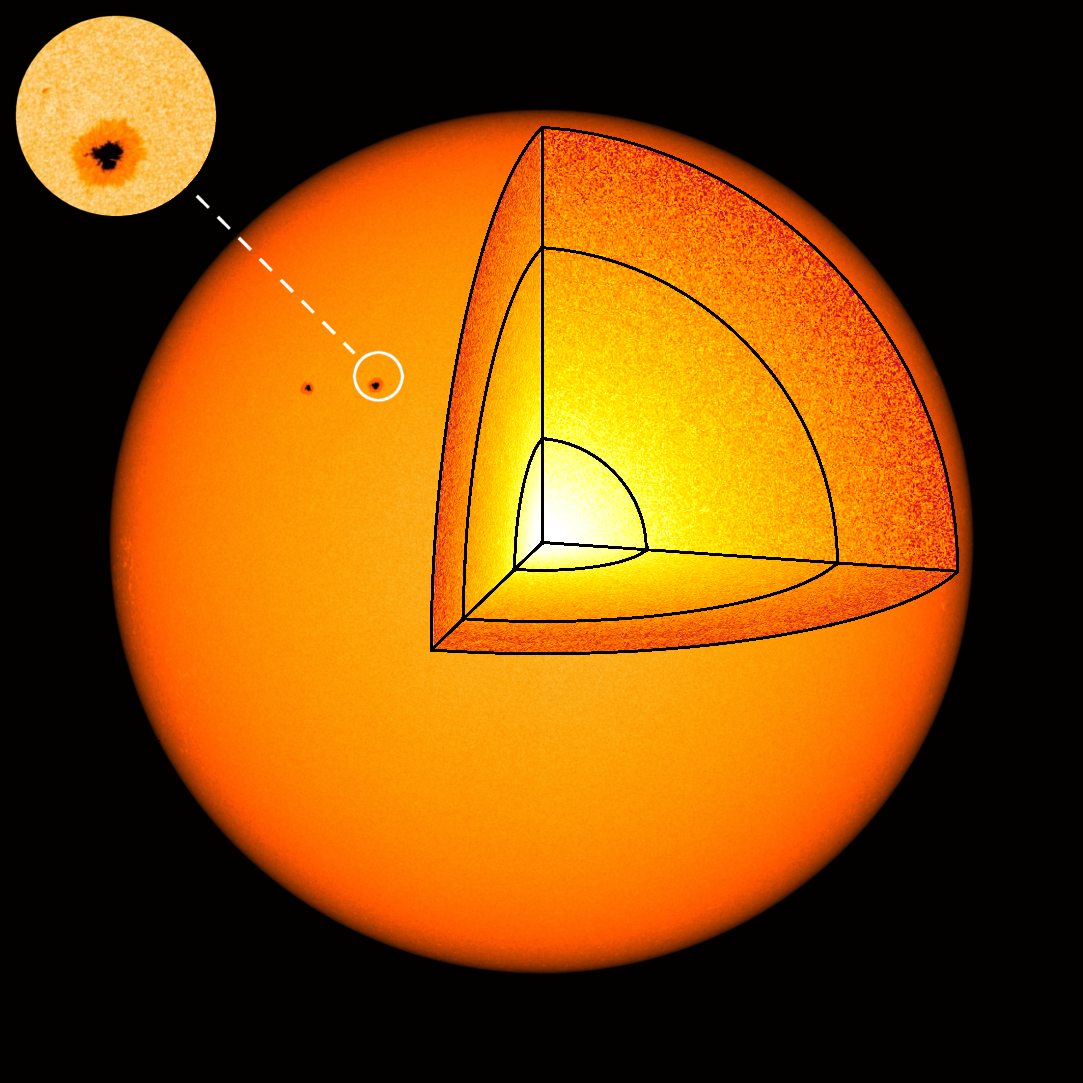
\includegraphics[width=0.6\textwidth]{figures_of_mine/schemata/sun_interior_HMIIC.png}
	}{
		\caption[\lofimage{figures_of_mine/schemata/sun_interior_HMIIC.png}I created this figure based on a SDO/HMI continuum image, credit: NASA/SDO and the AIA, EVE and HMI science teams.]
		{Image of the photosphere from 20~March~2016 together with a schema of the solar interior structure. The inset shows the granular surface with a sunspot. I created this figure based on a SDO/HMI continuum image, credit: NASA/SDO and the AIA, EVE and HMI science teams.}
		\label{fig:sun_interior_HMIIC}
	\addtocontents{lof}{\smallskip\protect\center I created the figure from NASA images.\medskip}
	}
\end{figure}

%%% chromosphere + corona + CMEs
Above the photosphere at the base of the chromosphere, the temperature declines to its solar minimum of \SI{3800}{\K} until it rises to \numrange{2}{3}~million~kelvins in the corona \citep{Billings1959,Liebenberg1975}. Up to now, it is not fully understood how the corona is so much hotter than the underlying chromosphere -- this question is known as the coronal heating problem \citep{Klimchuk2006,McComas2007,Fox2015}. The energy transfer mechanisms that are generally postulated are magnetic reconnections, wave heating and type~II spicules, or a combination of these \citep{Cranmer2017}.

The chromosphere is a \SI{2000}{\km} thick region, whose features -- numerous spicules, filaments, and prominences -- can reach far into the corona. They consist of chromospheric material, channeled by the solar magnetic field, and are enveloped by a thin transition region where the temperature jumps up from about \SI{30000}{\K}\footnote{NASA Sun fact sheet: \urlfoot{https://nssdc.gsfc.nasa.gov/planetary/factsheet/sunfact.html}} to coronal temperatures. Reconnection of magnetic field lines can result in the eruption of filaments into the corona and beyond, termed coronal mass ejections (CMEs), see also \autoref{sec:coronal_mass_ejections}. Details of chromospheric features are shown in \autoref{fig:sun_atmosphere} -- the images were taken on the same day as in \autoref{fig:sun_interior_HMIIC}.
\begin{figure}[htb]
	\fcapside[\FBwidth]{
		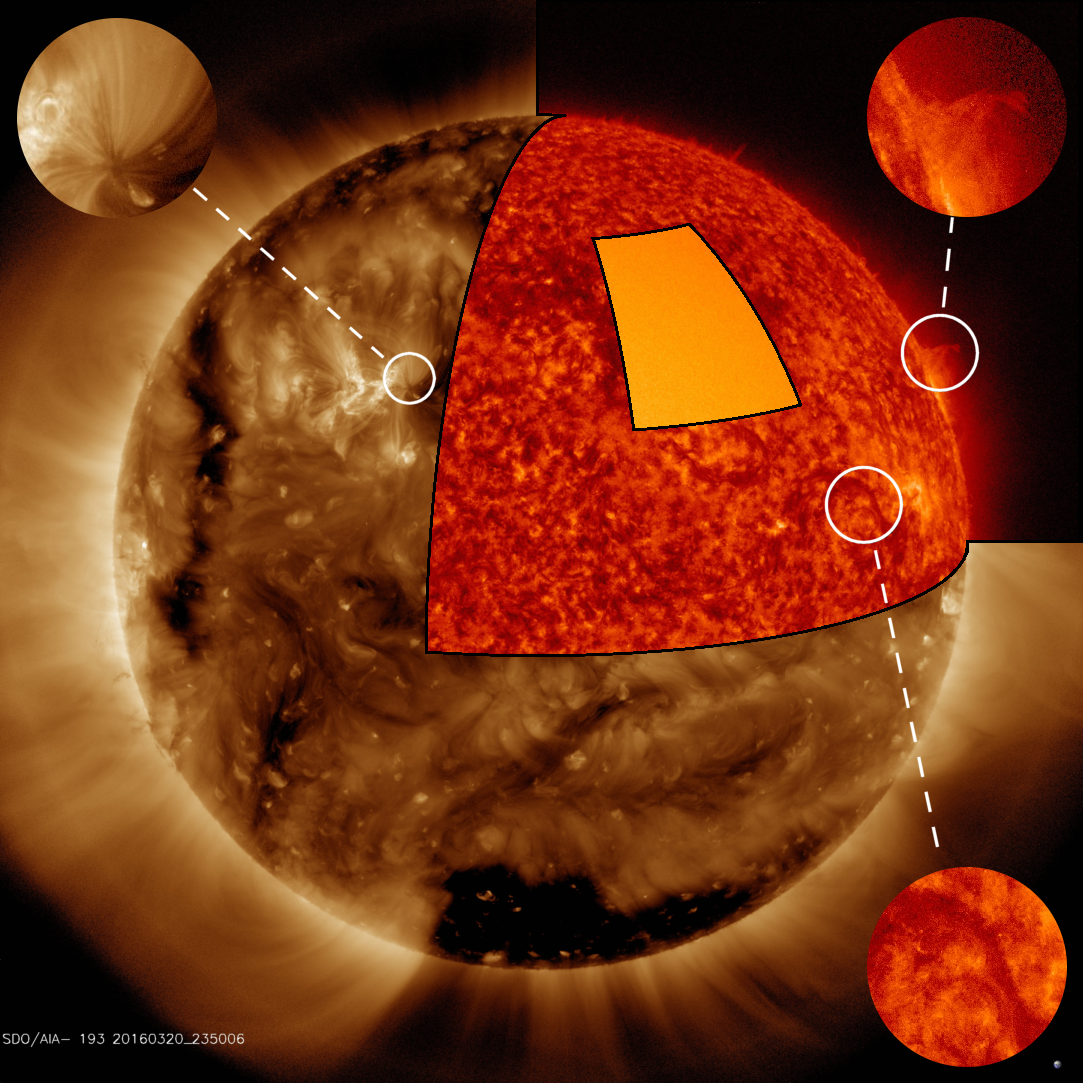
\includegraphics[width=0.6\textwidth]{figures_of_mine/schemata/sun_atmosphere.png}
	}{
		\caption[\lofimage{figures_of_mine/schemata/sun_atmosphere.png}I created this figure based on SDO/AIA images, credit: NASA/SDO and the AIA, EVE and HMI science teams.]
		{Composite image of the solar atmosphere from 20~March~2016 and some details of its features. Corona, chromosphere and photosphere are seen in wavelengths of \SI{193}{\angstrom}, \SI{304}{\angstrom}, and continuum. Chromospheric spicules are visible on the northern limb. The enlargements on the right show a prominence and a filament. The dark region at the south pole is a coronal hole. The left inset shows details of the active region belonging to the sunspots shown in \autoref{fig:sun_interior_HMIIC}. I created this figure based on SDO/AIA images, credit: NASA/SDO and the AIA, EVE and HMI science teams.}
		\label{fig:sun_atmosphere}
	}
	\addtocontents{lof}{\smallskip\protect\center I created the figure from NASA images.\medskip}
\end{figure}

%%% coronal holes
The Sun's atmosphere is dominated by the varying small- and large-scale solar magnetic field configuration. There are regions where the magnetic field lines arch back to the surface and regions with open field lines. In the latter areas, the coronal plasma can -- guided by the field -- escape into space. Thus, these coronal areas are less dense, cooler and therefore appear darker in extreme ultraviolet (EUV) and are called coronal holes (CHs). In \autoref{fig:sun_atmosphere} such a coronal hole is visible at the solar south pole.

%%% corona
From Earth, the faint corona and chromosphere can only be observed during eclipses, due to the brightness of the solar disk. There are three effects contributing to the visibility of the corona: photons scattering off of free electrons, producing a continuous spectrum; photons scattering off of dust particles, their spectrum contains Fraunhofer absorption lines; and ion spectral emission lines -- these contributions to the corona are termed K-, F- and E"~corona\footnote{K from kontinuierlich (continuous in German), F from Fraunhofer, and E from emission.}.
% the so-called K-, F- and E"~corona (K kontinuierlich, F Fraunhofer, E emission).\\
% K-corona: photon scattering off free electrons --> coronagraphs\\
% F-corona: photon scattering off dust particles; contains Fraunhofer absorption lines; expands in ecliptic as zodiacal light --> coronagraphs\\
% E-corona: ion spectral emission lines; reveals coronal composition --> images\\
Images from solar eclipses reveal the coronal plasma, shaped by the magnetic field, and red prominences from the chromosphere. The solar eclipse imaged in \autoref{fig:Tse2008_500_mo1} shows the magnetic field's dipole structure and the equatorial streamer belt, characteristic for a quiet Sun during cycle minimum.
\begin{figure}[htb]
	\fcapside[\FBwidth]{
		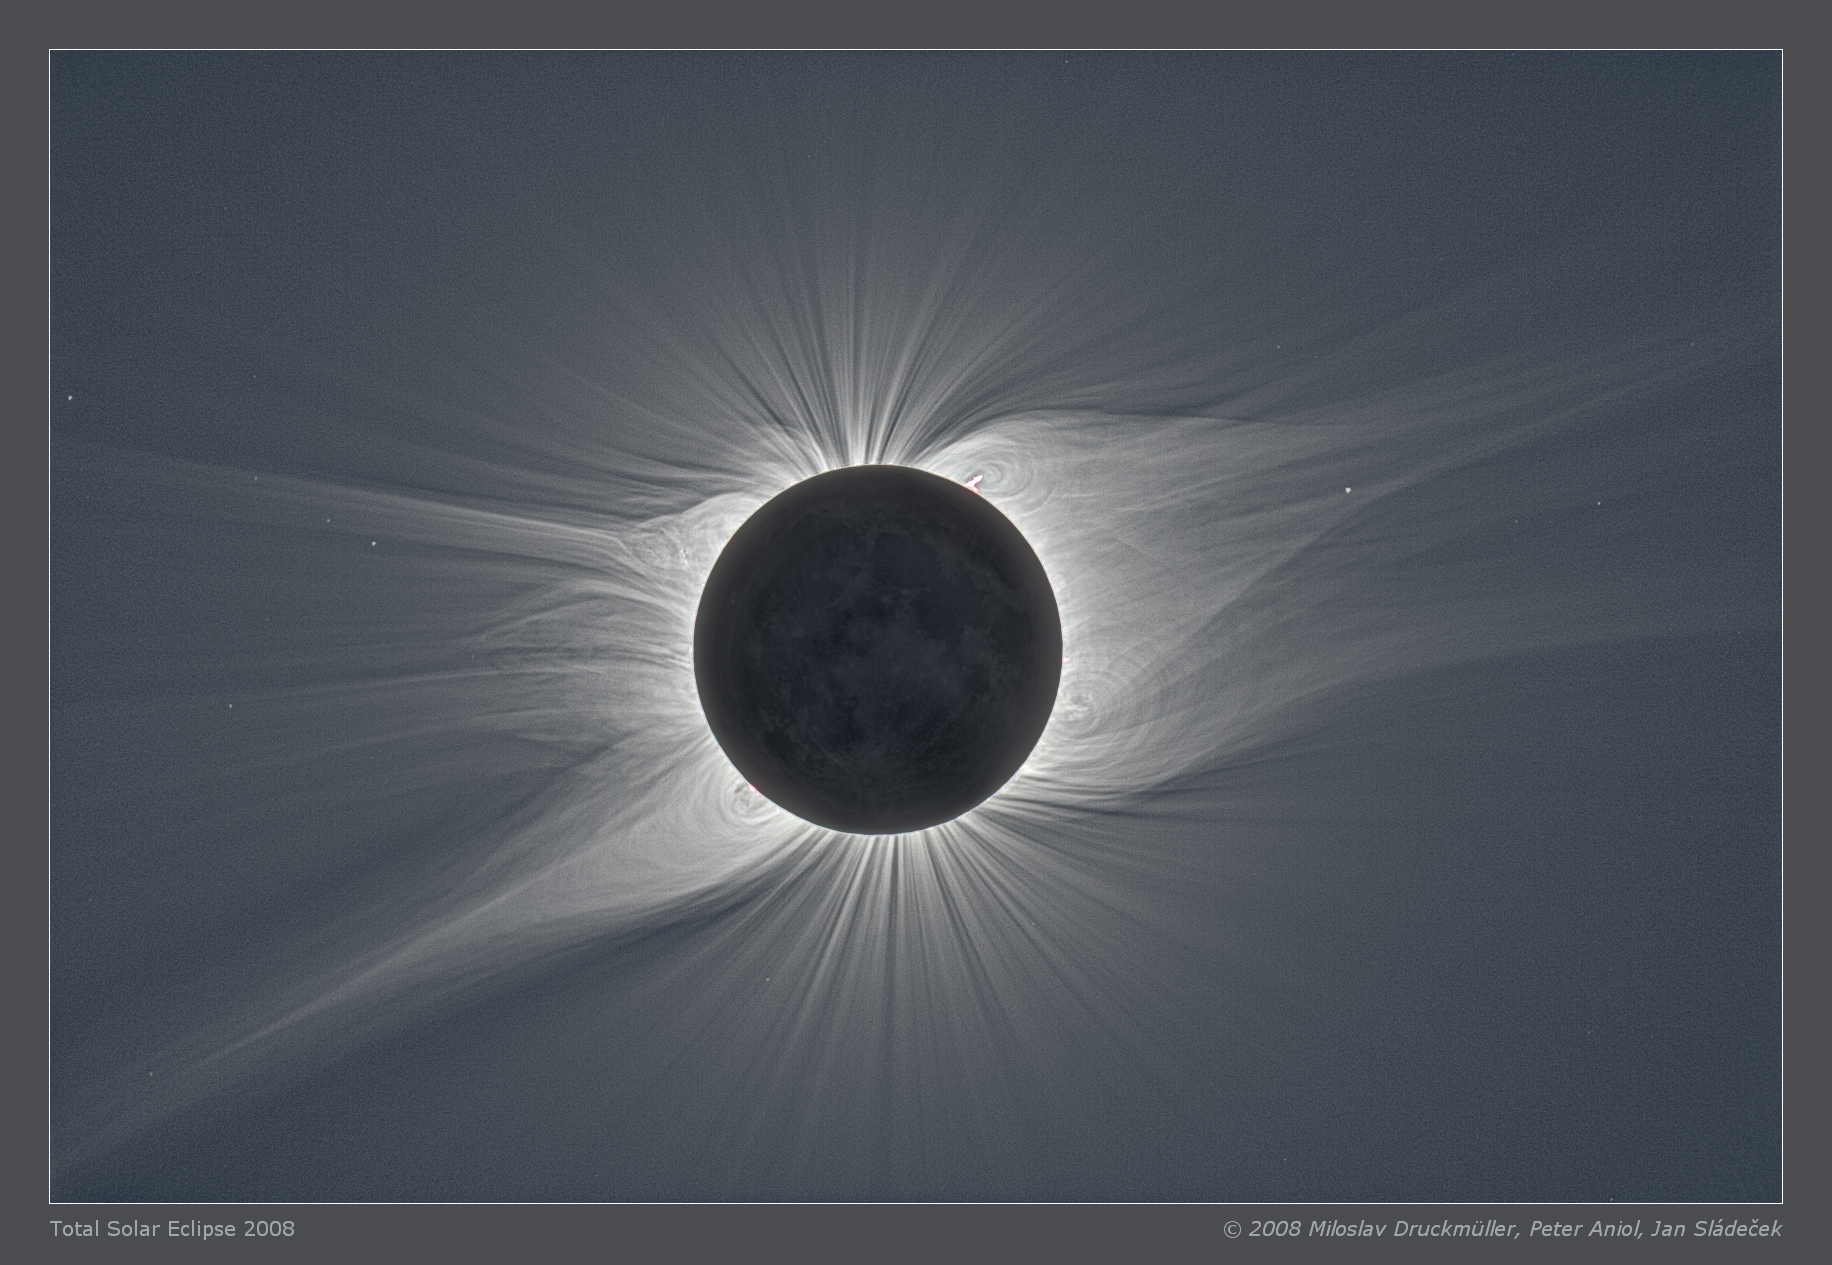
\includegraphics[width=0.55\textwidth]{figures_of_others/images/Tse2008_500_mo1.png}
	}{
		\caption[\lofimage{figures_of_others/images/Tse2008_500_mo1.png}Credit: \href{http://www.zam.fme.vutbr.cz/~druck/Eclipse/}{Miloslav Druckmüller, Peter Aniol, Jan Sládeček}, 2008, reproduced with permission.]
		{Total solar eclipse image of the inner corona up to a distance of five solar radii. The picture was taken in Mongolia, 1~August~2008 and is processed from multiple images. Credit: \href{http://www.zam.fme.vutbr.cz/~druck/Eclipse/}{Miloslav Druckmüller, Peter Aniol, Jan Sládeček}, 2008, reproduced with permission.}
		\label{fig:Tse2008_500_mo1}
	}
	\addtocontents{lof}{\smallskip\protect\center See the following email correspondence.
		\protect\lstinputlisting{figures_of_others/permissions/Druckmuller_permission.txt}\medskip
	}
\end{figure}
%figure source: http://www.zam.fme.vutbr.cz/~druck/Eclipse/Ecl2008m/Tse2008_500_mo1/Hr/Tse2008_500_mo1.png

%%% solar wind + heliosphere
Due to the high coronal temperatures, plasma escapes the solar gravitational field \citep{Parker1958} with velocities of \SIrange{200}{800}{\km\per\s}. Its acceleration is linked to the coronal heating -- however, the exact location and mechanism of this process remain unknown \citep{Hollweg1985,McComas2007,Fox2015,Cranmer2017}. The magnetic field becomes too weak to guide the coronal plasma at a distance of a few solar radii. From this so-called 'source surface', the solar wind flows radially outward into space until it reaches the termination shock. Eventually it collides with the local interstellar medium, creating the boundary of the heliosphere, the heliopause. The heliopause is expected to be a bubble of either a teardrop or croissant shape, caused by the Sun's relative velocity of \SI{23}{\km\per\s} with respect to the local interstellar medium \citep{Owens2013, Opher2015}. However, \citet{McComas2012} show that this velocity is too slow to form a leading bow shock. Measurements of the Voyager~1 and Voyager~2 spacecraft indicate their passage of the termination shock at about 94~astronomical units (au)\footnote{One astronomical unit is defined as \SI{149597870.7}{\km}, see also Appendix~\ref{sec:astronomical_constants}} and \SI{84}{\au} respectively, entering the heliosheath region \citep{Owens2013}. \citet{Gurnett2013} report that in 2012 Voyager~1 actually crossed the heliopause into interstellar space at a solar distance of \SI{121}{\au}. The heliosphere and its surrounding flow structure is illustrated in \autoref{fig:Owens2013_Heliosphere_screenshot}.
\begin{figure}[h]
	\fcapside[\FBwidth]{
		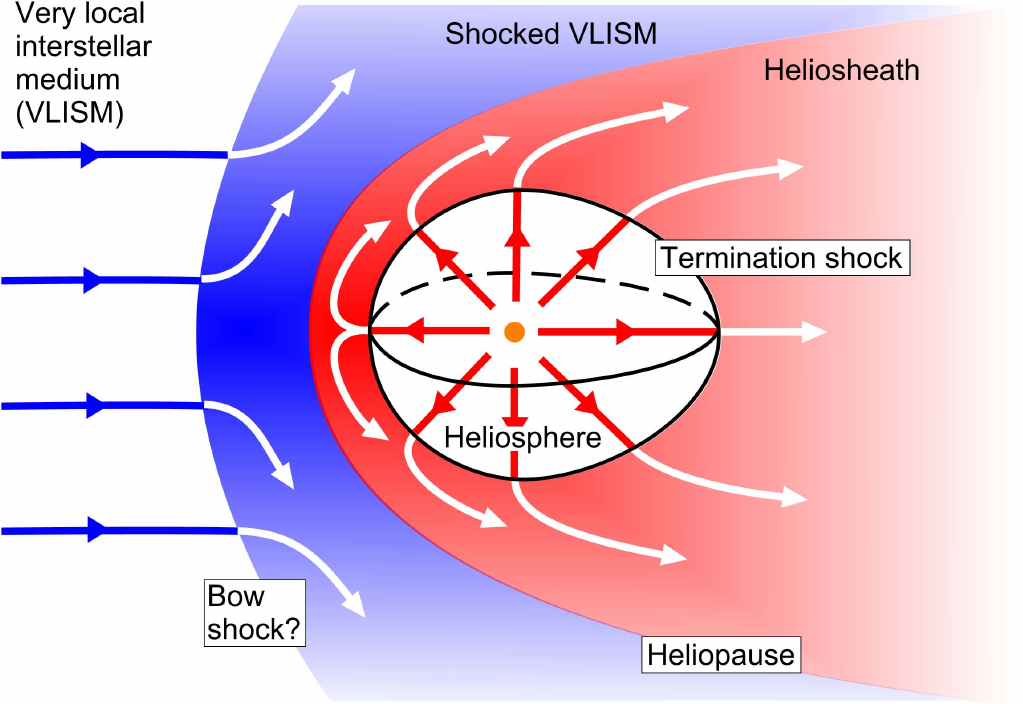
\includegraphics[width=0.55\textwidth]{figures_of_others/images/Owens2013_Heliosphere_screenshot.png}
	}{
		\caption[\lofimage{figures_of_others/images/Owens2013_Heliosphere_screenshot.png}Credit: {\citet[Fig.~9]{Owens2013}}, licensed under \href{https://creativecommons.org/licenses/by-nc/3.0/de/}{CC BY-NC 3.0 DE}.]
		{Schema of the heliosphere and its surrounding flow structure, formed by the interaction of the solar wind (red) with the local interstellar medium (blue) at the heliopause. Credit: {\citet[Fig.~9]{Owens2013}}, licensed under \href{https://creativecommons.org/licenses/by-nc/3.0/de/}{CC BY-NC 3.0 DE}.}
		\label{fig:Owens2013_Heliosphere_screenshot}
	}
	\addtocontents{lof}{\smallskip\protect\center See the following RightsLink request result.\protect\\
		\protect\fbox{\protect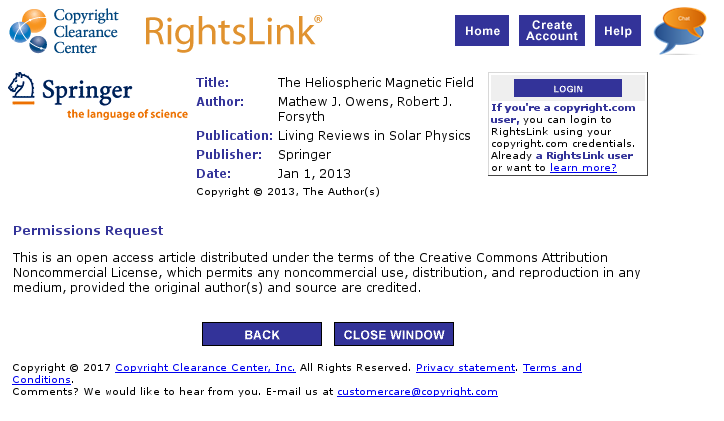
\includegraphics[width=0.7\textwidth]{figures_of_others/permissions/permission_request_Owens2013.png}}\protect\\
		\medskip
	}
\end{figure}
%Owens2013 figure permission request: open access article

\pagebreak

%%% solar wind influence + space weather
On its way outwards through the solar system, the solar wind -- carrying the solar magnetic field -- interacts with the planets, their magnetic fields and other solar system bodies. This has a number of effects, for instance disturbances in planetary magnetic fields with appearance of aurorae and enhanced radiation, atmospheric losses, and stripping of cometary tails. Some of these effects can have disruptive consequences for humans and their technology, creating a high interest in understanding space weather and forecasting its effects, the topic of space weather is further addressed in \autoref{sec:space_weather}. The magnitudes of these effects depend highly on spatial and temporal variations in the solar wind, which are rooted in the dynamics of the solar magnetic field, described in the following sections.

%%%%%%%%%%%%%%%%%%%%%%%%%%%%%
%\section{Stars/Beginning}
% introduction leading to stars; beginning from universe/big bang\\
% gravitational contraction of rotating nebula\\
% -> fusion burning; energy production\\
% In its core it fuses hydrogen to helium; 15.7~million~K; inner 25~\%\\
% energy transport -> radiation zone; up to 70~\%\\
% tachocline ~2~million~K\\
% energy transport by convection -> convection zone; up to surface\\
% convective granulation\\
% photoshere 4400--6600~K, effective black body temperature 5777~K; spectral class\\
% (herzsprung russell diagram)\\
% chromosphere... (solar atmosphere figure)\\
% transition region\\
%corona 1--3~million~K temperature (coronal heating problem)\\
% coronal holes: open magnetic field lines, solar wind\\
% heliosphere, shock with interstellar medium (ISM); Voyager\\

%%%%%%%%%%%%%%%%%%%%%%%%%%%%%
%big bang
%to formation of stars
%to ISM in our galaxy
%to formation of Sun
%Sun's inner structure (energy production and transport)
%its surface (radiation, spectral class)
%its outer structure (chromosphere, corona, solar wind, heliosphere)
%its heliosphere (termination shock with ISM, Voyager measurements)
%%%%%%%%%%%%%%%%%%%%%%%%%%%%%


\section{Solar dynamo}
\label{sec:solar_dynamo}
%%% differential rotation + solar magnetic field origin
The conservation of the angular momentum in the contracting molecular cloud led to a rotation of the Sun. Although the Sun experiences a minor loss of angular momentum due to solar wind \citep{Weber1967}, its rotation still has a current average period of about 25~days. The radial convective motion within the solar interior above the tachocline leads to a transport of momentum away from the rotation axis and therefore to a slower polar and faster equatorial rotation in the convection zone \citep{Miesch2005}. This differential rotation is visible on the surface and was first discovered from sunspot observations by \citet{Scheiner1630}. With a rotation period of about 34~days, the poles have a lag of almost 9~days (for further information on solar rotation see Appendix~\ref{sec:solar_surface_differential_rotation}). The differential rotation in the solar interior can be inferred from helioseismological observations. Below the differential rotation of the convection zone, a nearly solid rotation with a period of about \SI{26.6}{days} (this corresponds to a frequency of \SI{435}{\nano\hertz}) exists in the radiation zone, as shown in \autoref{fig:Miesch2005_fig1a_interior_diff_rot}.
\begin{figure}[htb]
	\begin{floatrow}
		\ffigbox{
			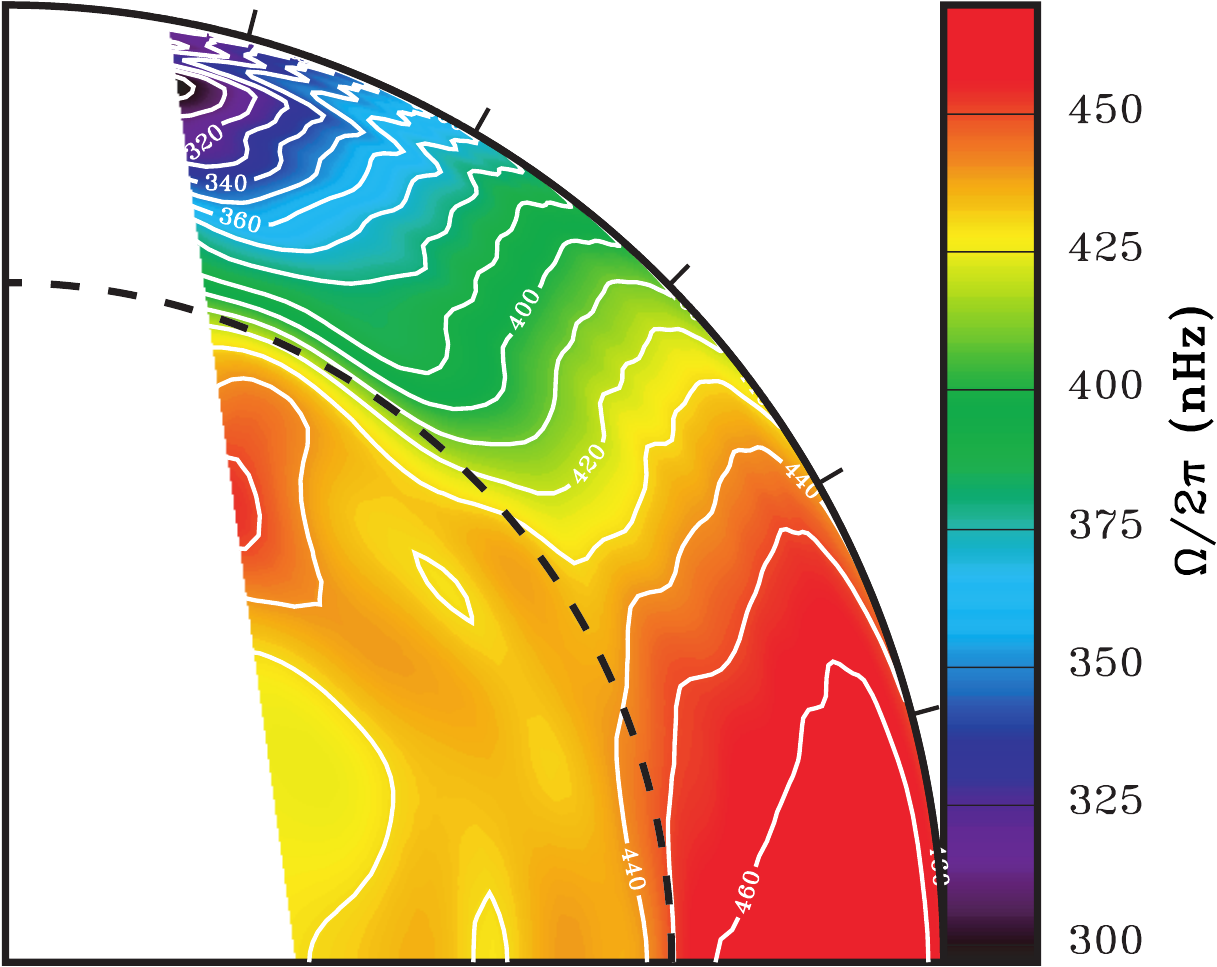
\includegraphics[width=0.5\textwidth]{figures_of_others/images/Miesch2005_fig1a_interior_diff_rot.png}
		}{
			\caption[\lofimage{figures_of_others/images/Miesch2005_fig1a_interior_diff_rot.png}Credit: {\citet[Fig.~3]{Thompson2003}}, \textcopyright~Annual~Reviews, reproduced with permission.]
			{Rotation frequency profile of the solar interior. The location of the tachocline is indicated by the dashed line. The rotation frequency is inferred from helioseismology via observations from the Michelson Doppler Imager (MDI) at the Solar and Heliospheric Observatory (SOHO) spacecraft. Credit: {\citet[Fig.~3]{Thompson2003}}, \textcopyright~Annual~Reviews, reproduced with permission.}
			\label{fig:Miesch2005_fig1a_interior_diff_rot}
			%(\citet[Fig.~1\,a]{Miesch2005}; based on \citet[Fig.~3]{Thompson2003})
			%Thompson2003 permission request: permission not required
		}
		\addtocontents{lof}{\smallskip\protect\center See the following RightsLink request result.\protect\\
			\protect\fbox{\protect
\includegraphics[width=0.7\textwidth]{figures_of_others/permissions/permission_request_Thompson2003.png}}\protect\\
			\bigskip
		}
		\ffigbox{
			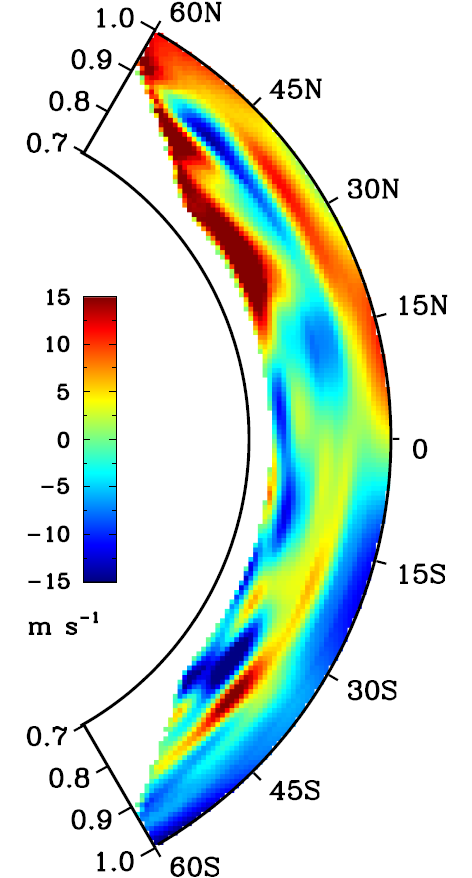
\includegraphics[width=0.28\textwidth]{figures_of_others/images/Zhao2013_meridional_flow.png}
		}{
			\caption[\lofimage{figures_of_others/images/Zhao2013_meridional_flow.png}Credit: {\citet[Fig.~4, panel~(a), I moved the colorbox]{Zhao2013}}, \textcopyright~AAS, reproduced with permission.]
			{Meridional flow velocity profile in part of the convection zone. Positive values are directed towards north. The velocity is inferred from helioseismology via observations from the Helioseismic Magnetic Imager (HMI) at the Solar Dynamics Observatory (SDO) spacecraft. Credit: {\citet[Fig.~4, panel~(a), I moved the colorbox]{Zhao2013}}, \textcopyright~AAS, reproduced with permission.}
			\label{fig:Zhao2013_meridional_flow}
			%Zhao2013 permission request: permission granted.
		}
		\addtocontents{lof}{\smallskip\protect\center See the following email correspondence.
			\protect\lstinputlisting{figures_of_others/permissions/Zhao2013_permission.txt}\medskip
		}
	\end{floatrow}
\end{figure}
%Angular velocity profile in the solar interior inferred from helioseismology (after Thompson et al., 2003). In panel (a), a 2D (latitude-radius) rotational inversion is shown based on the subtractive optimally localized averaging (SOLA) technique. All inversions are based on data from the Michelson Doppler Imager (MDI) instrument aboard the SOHO spacecraft, averaged over 144 days. Inversions become unreliable close to the rotation axis, represented by white areas in panel (a). Note also that global modes are only sensitive to the rotation component which is symmetric about the equator (courtesy M.J. Thompson \& J. Christensen-Dalsgaard).

%%% magnetic field dynamo mechanism
Turbulent plasma motions from convective flows in the convection zone generate and carry disorganized magnetic flux. The large rotational shear at the tachocline stretches and amplifies the magnetic fields to strong coherent toroidal flux ($\omega$-effect) with intensities of the order \SIrange{1}{10}{\tesla}. These toroidal fields, generated near the bottom of the convection zone, can be stored in a deep magnetic layer located in the stably stratified region below the convection zone \citep{Ossendrijver2003}. The stronger flux ropes become buoyant and rise to the surface. The Coriolis force twists them systematically on their way through the convection zone ($\alpha$-effect). The twist is stronger at higher latitudes (Joy's law). Then the flux ropes emerge in the photosphere as bipolar active regions of opposite magnetic polarity -- the stronger ones forming pairs of sunspots, as seen in \autoref{fig:bipolar_region_HMIB_HMIIF}.
\begin{figure}[htb]
	\centering
	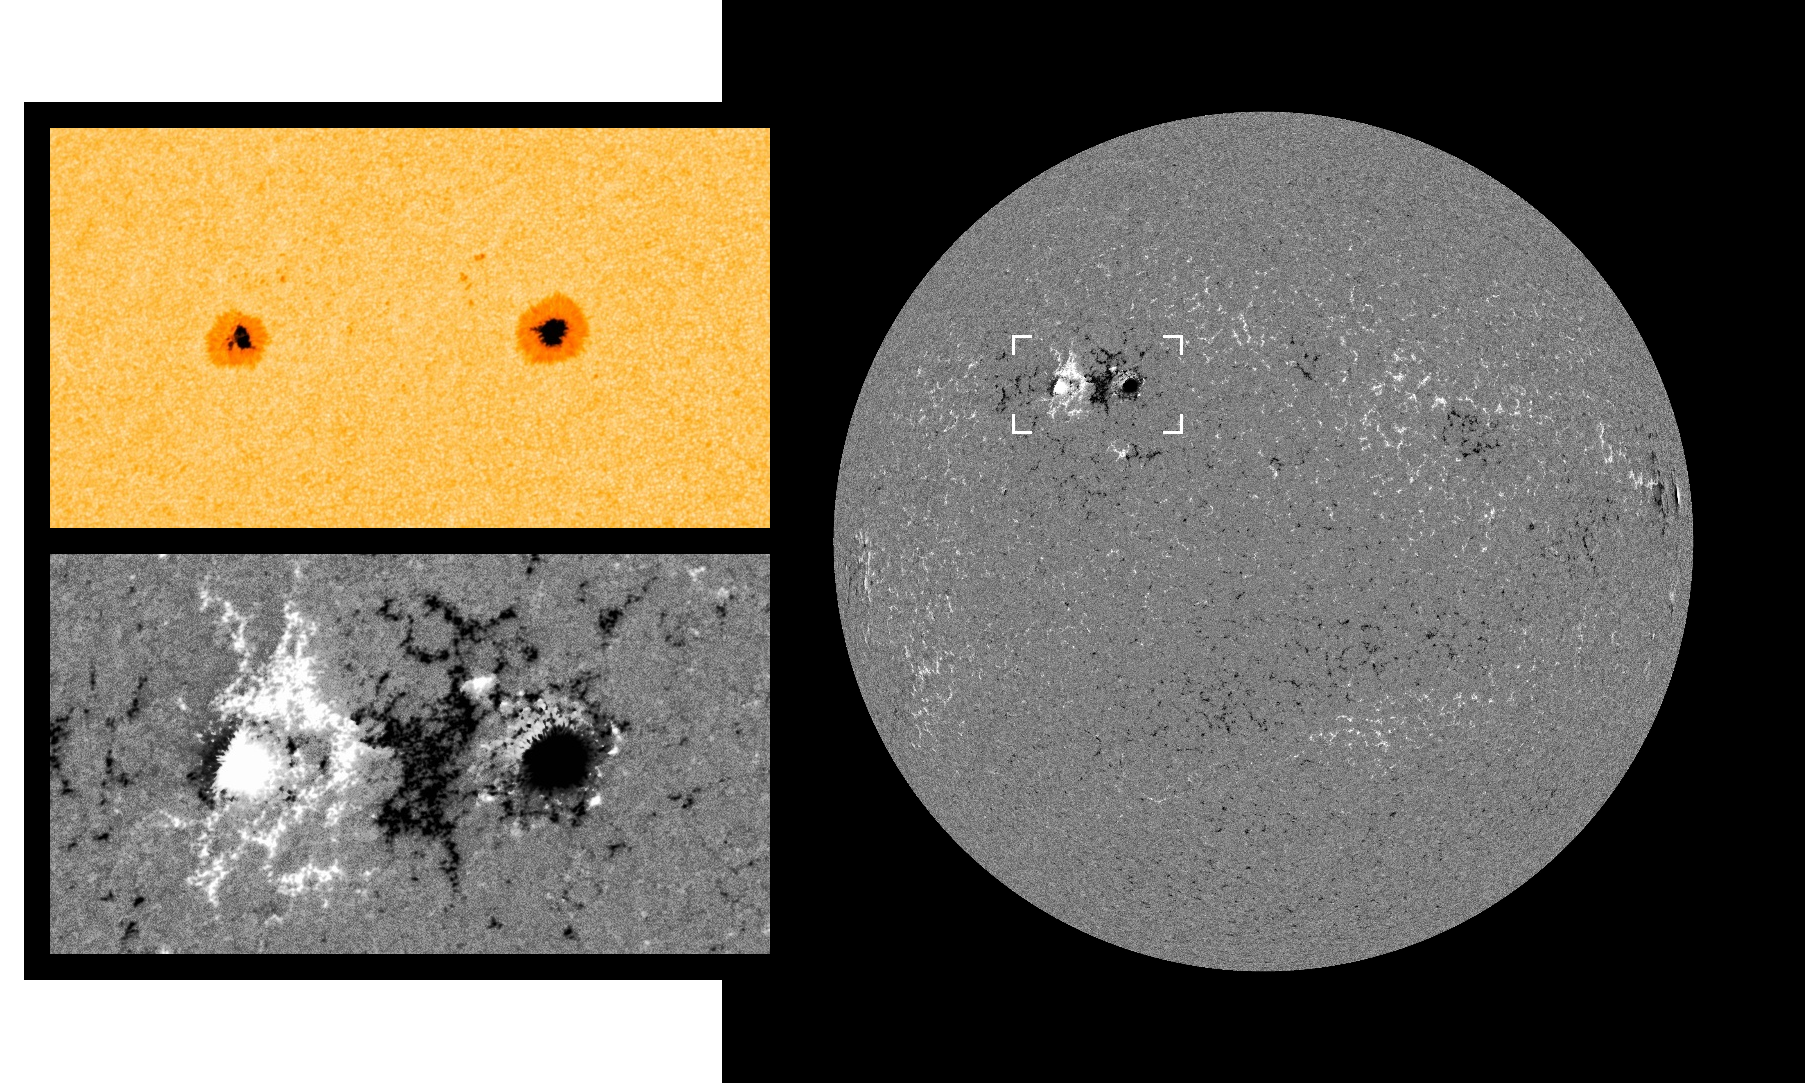
\includegraphics[width=\textwidth]{figures_of_mine/schemata/bipolar_region_HMIB_HMIIF.png}
	\caption[\lofimage{figures_of_mine/schemata/bipolar_region_HMIB_HMIIF.png}I created the figure based on SDO/HMI continuum and magnetogram images from 20~March~2016, credit: NASA/SDO and the HMI science team.]
	{Continuum image of the two sunspots pictured in \autoref{fig:sun_interior_HMIIC} (top left), magnetogram from the same region (bottom left), and magnetogram from the whole solar disk (right). The magnetogram shows the polarity of the line-of-sight magnetic field component at the photosphere (black/white: inward/outward polarity). The highly concentrated magnetic flux at the sunspots is visible as well as the extended bipolar magnetic field structure of the whole active region, which is divided by the so-called magnetic neutral line. The solar disk has the same size as in \autoref{fig:sun_interior_HMIIC}. I created the figure based on SDO/HMI continuum and magnetogram images from 20~March~2016, credit: NASA/SDO and the HMI science team.}
	\label{fig:bipolar_region_HMIB_HMIIF}
	\addtocontents{lof}{\smallskip\protect\center I created the figure from NASA images.\medskip}
\end{figure}
% HMI is a vector magnetogram, but the public sources say that the magnetogram shows a line-of-sight magnetic field.
Turbulent convective diffusion of this surface flux contributes to the build-up of poloidal fields. Their resulting polarity is opposite to the prevailing global field due to the directional way the rotational shear at the tachocline and the Coriolis force in the convection zone act. Fluctuating motions further amplify the mean fields in these processes. This solar $\alpha$-$\omega$-dynamo is thought to create the major part of the solar magnetic field. Still, with regard to the magnetic field's high variability, the long-term mean fields are governed by intermittent localized structures, that is, active regions, filaments and coronal loops \citep{Miesch2005}.	%Miesch2005 p.~18 + p.~31

% the $\alpha$-$\omega$-dynamo, see \autoref{fig:EOSFIG2_modified}\\
% \begin{figure}[htb]
% 	%\centering
% 	\fcapside[\FBwidth]{
% 		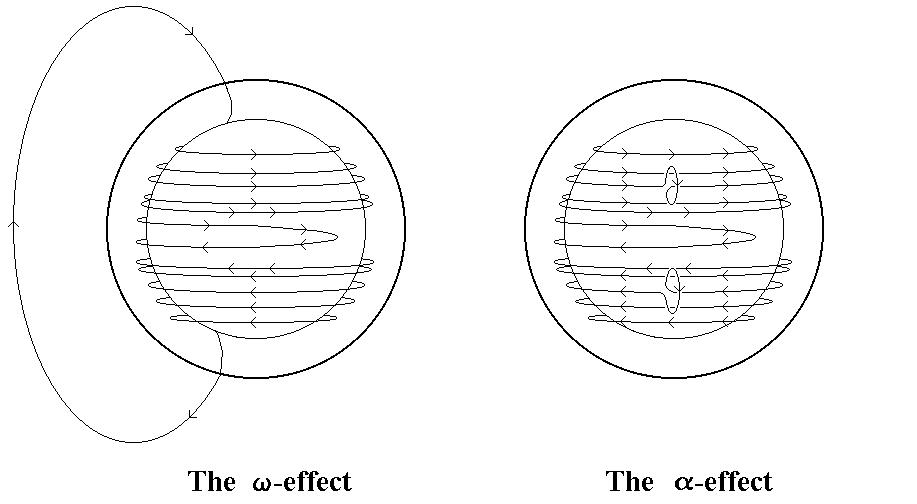
\includegraphics[width=0.5\textwidth]{figures_of_others/images/EOSFIG2_modified.png}
% 	}{
% 		\caption{Schemata of the $\omega$ and the $\alpha$-effects. figure really necessary? get permission...}
% 		\label{fig:EOSFIG2_modified}
% 	}
% \end{figure}
%http://certificate.ulo.ucl.ac.uk/modules/year_one/NASA_MSFC/solar_physics/dynamo.htm
%https://solarscience.msfc.nasa.gov/images/EOSFIG2.GIF

% switching between states of strong poloidal and toroidal field\\
% poloidal field + diff. rot. => toroidal field ($\Omega$-effect)\\
% the solar dynamo: (toroidal to poloidal field)\\
% - turbulent plasma motions from convective flows generate disorganized magnetic fields\\
% - differential shear at tachocline amplifies fields to strong coherent toroidal flux ($\Omega$-effect); magnetic layer located at the base of the convection zone\\
% - stronger flux ropes raise to surface (buoyantly)\\
% - Coriolis force twists them systematically, stronger at higher latitudes\\
% - twisted tubes emerge on the surface as bipolar active regions\\
% - amplification of mean fields by fluctuating motions ($\alpha$-effect) and turbulent diffusion create large-scale poloidal field\\


\section{Solar activity cycle}
\label{sec:solar_activity_cycle}
%%% convection cycle + solar surface magnetic field + solar cycle
Helioseismic measurements reveal that the large-scale convective flow is aggregated into large convection cells with slow meridional flows of a few \si{\m\per\s}, as can be seen from \autoref{fig:Zhao2013_meridional_flow}. A poleward subsurface flow and equatorward backflow beneath with a further poleward flow below are detected within each hemisphere, comprising a stacked double-cell profile \citep{Zhao2013}. The meridional circulation flow speed has a major influence on the average 22-year period of the emerging magnetic flux at the solar surface, known as Hale cycle. This period varies and is influenced by the stochastic emergence rate and tilts of active regions and the diffusion from random convective motions \citep{Hathaway2016}. The surface magnetic field configuration changes within one period from a dipole structure to a reversed dipole structure with opposite polarity and back, completing a so-called Babcock-Leighton dynamo cycle. Thus, the transition time from one dipole state to the next lasts about 11~years, this period is defined as one solar cycle.
%http://www.solarcyclescience.com/forum/viewforum.php?f=9

%%% butterfly pattern
In the transition phase, magnetic flux emerges in belts above and below the solar equator, manifesting as bipolar active regions with sunspots, resulting in a toroidal/multipolar structured magnetic field. Sunspots appear at about \SI{+-20}{\degree} latitude at the beginning of a cycle, this shifts towards lower latitudes at the end of a cycle. Thus, the plot of sunspots over latitude and time reveals a butterfly pattern \citep{Maunder1904}. This butterfly pattern appears in surface radial magnetic field observations as well, see \autoref{fig:Hathaway_magbfly}. The leading polarity of bipolar regions is opposite in both hemispheres and the leading polarity changes with each solar cycle, this is called Hale's polarity law. The emerging flux is carried by the slow meridional surface flow poleward, canceling the current dominating polar field polarity and eventually resulting in the polar field switch \citep{Hathaway2015}.
\begin{figure}[htb]
	\centering
	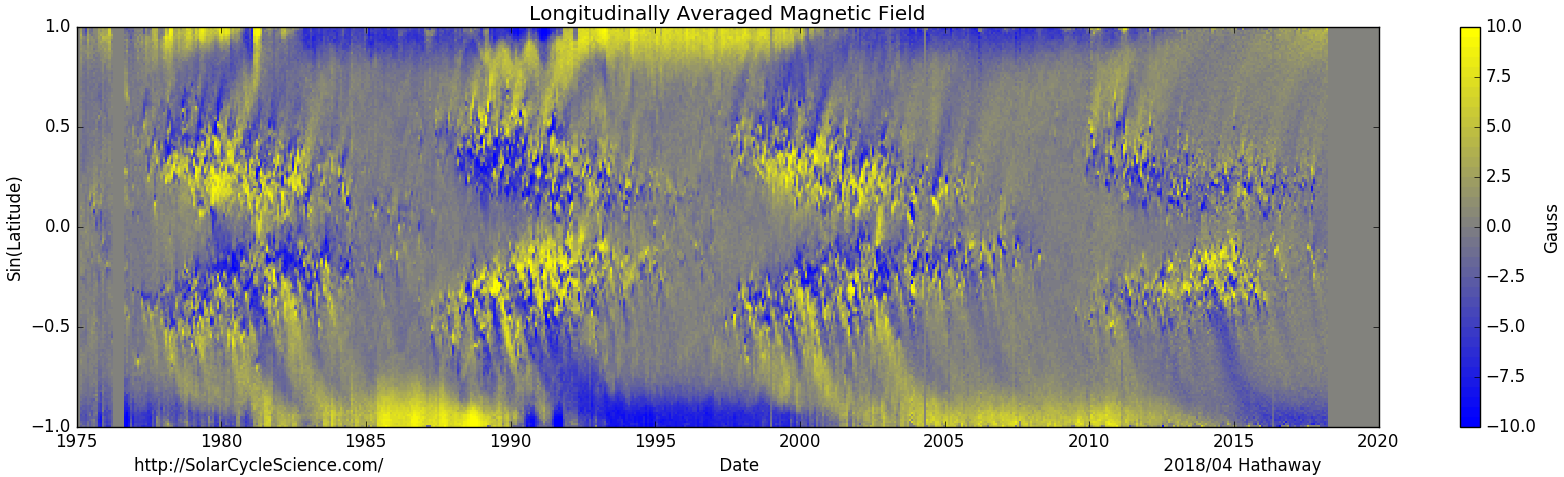
\includegraphics[width=\textwidth]{figures_of_others/images/Hathaway_magbfly_201804_cropped.png}
	\caption[\lofimage{figures_of_others/images/Hathaway_magbfly_201801_cropped.png}Courtesy of David~Hathaway, \href{http://solarcyclescience.com/solarcycle.html}{Solar Cycle Science}, 2018, updated version of {\citet[Fig.~17]{Hathaway2015}}.]
	{Magnetic butterfly diagram of the longitudinally averaged radial magnetic field on the solar surface. Yellow represents an outward directed magnetic field (positive), blue inward (negative). The data is obtained from instruments on Kitt~Peak National Observatory and from the MDI at the SOHO spacecraft. Courtesy of David~Hathaway, \href{http://solarcyclescience.com/solarcycle.html}{Solar Cycle Science}, 2018, updated version of \citet[Fig.~17]{Hathaway2015}.}
	\label{fig:Hathaway_magbfly}
	\addtocontents{lof}{\smallskip\protect\center See the following email correspondence.\medskip
		\protect\lstinputlisting{figures_of_others/permissions/Hathaway_permission.txt}
	}
\end{figure}
%Hathaway 2015 permission request: open access article
%figure source:	http://solarscience.msfc.nasa.gov/images/magbfly.jpg
%Hathaway website permission request: requested
%figure source:	http://solarcyclescience.com/solarcycle.html

%%% sunspot number
Since regions of strong magnetic flux are visible as sunspots on the photosphere, they were known well before the common era by Greek and Chinese scholars \citep{Clark1978,Vaquero2007}. %greek sunspot observation: http://adsabs.harvard.edu/abs/2007JBAA..117..346V
Systematic sunspot observations exist since 1610, shortly after the invention of the telescope. In 1843 Schwabe discovered the 11-year periodicity in the sunspot occurrence \citep[p.~124]{Schroeder2004}. In 1848 Wolf introduced the sunspot number (SSN) and the solar cycle number to record these cycles \citep{Hathaway2015}.	%the zeroth in 1749
Observations of the SSN show large variations in cycle length (9--14~years) and cycle amplitude with peak SSNs in the range 0--300 \citep{Hathaway2015} -- the monthly SSN from the last six solar cycles is displayed in \autoref{fig:ROB_SILSO_SSN_wolfmms_cropped}. There also exist long-term variations, such as secular cycles of different periodicity or the 70"~year Maunder~Minimum, during which from 1645 on almost no sunspots were observed, \citep{Maunder1890}.	%but: Zolotova2015: "The Maunder Minimum is Not as Grand as it Seemed to be"
The source of the variations in the solar cycle periods and amplitudes are variations in the meridional circulation, because their fluctuations are larger than those found in the differential rotation and in the convective motions \citep{Hathaway2015}.
\begin{figure}[htb]
	\fcapside[\FBwidth]{
		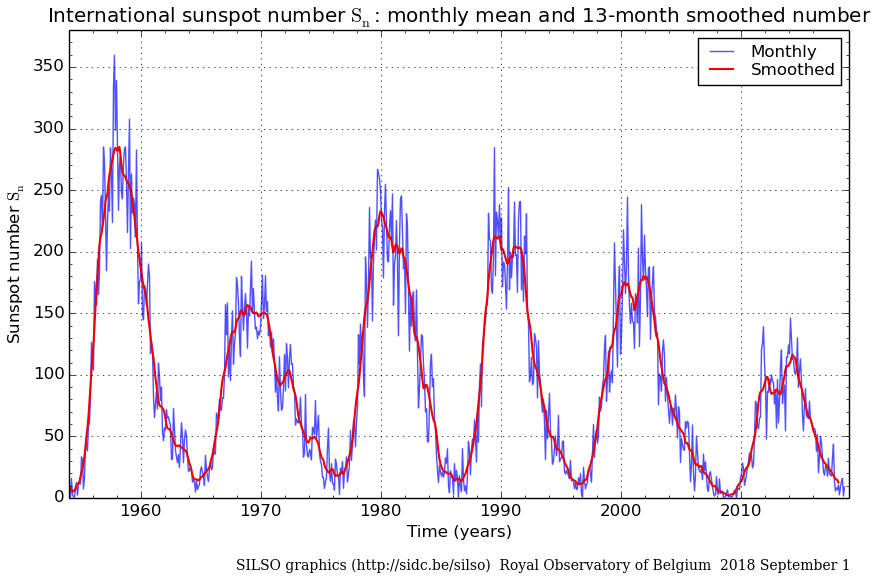
\includegraphics[width=0.6\textwidth]{figures_of_others/images/ROB_SILSO_SSN_wolfmms_cropped.png}
	}{
		\caption[\lofimage{figures_of_others/images/ROB_SILSO_SSN_wolfmms_cropped.png}Credit: \href{http://sidc.be/silso/monthlyssnplot}{SILSO data/image, Royal Observatory of Belgium, Brussels}, 2018.]
		{Monthly mean sunspot number (blue) and 13-month smoothed monthly sunspot number (red) for the last six solar cycles since 1954. Credit: \href{http://sidc.be/silso/monthlyssnplot}{SILSO data/image, Royal Observatory of Belgium, Brussels}, 2018.}
		\label{fig:ROB_SILSO_SSN_wolfmms_cropped}
	}
	\addtocontents{lof}{\smallskip\protect\center SILSO images can be freely downloaded as public data.\protect\footnote{SIDC/SILSO website, data policy at the bottom: \url{http://sidc.be/silso/home}}\medskip}
\end{figure}
%SIDC/SILSO permission request: permission not required
%image from:	http://sidc.be/silso/

%%% SSN prediction
As the SSN is commonly used as an indicator for solar activity, there exists interest in its prediction for the course of the actual and upcoming solar cycles. The continuing prediction of an already commenced activity cycle is reliable, but then the prediction of a cycle before it began is more difficult. Though, there are indications that the polar magnetic field strength during the preceding activity minimum is correlated to the strength of the next solar cycle \citep{Schatten1987}. However, \citet{Hathaway2016} suggest that the predictability of solar cycles is generally limited -- accumulated uncertainty produced by stochastic motions in the convection zone makes predictions further than the next solar cycle very unreliable.

\clearpage

\section{Coronal and heliospheric magnetic field}
\label{sec:coronal_and_heliospheric_magnetic_field}
%%% MBPs to canopy
The Sun's magnetic field governs the plasma movements in the corona and extends out into space, forming the heliospheric magnetic field (HMF). Its sources on the photosphere are bright points between the granules, which are detected in G-band (\SI{430}{\nano\meter}) images. They are identified as magnetic flux tubes with field strengths of \SIrange{100}{200}{\milli\tesla} \citep{Cranmer2005}. Together, these magnetic bright points cover around \SIrange{1}{2}{\%} of the solar surface and carry many times the flux that active regions do \citep{Sanchez_Almeida2010}. These thin flux tubes expand laterally in the low chromosphere and merge to homogeneous network fields, which expand and merge again to a large-scale canopy below the transition region (see \autoref{fig:Cranmer2005_fig1_ab}).
\begin{figure}[htb]
	\fcapside[\FBwidth]{
		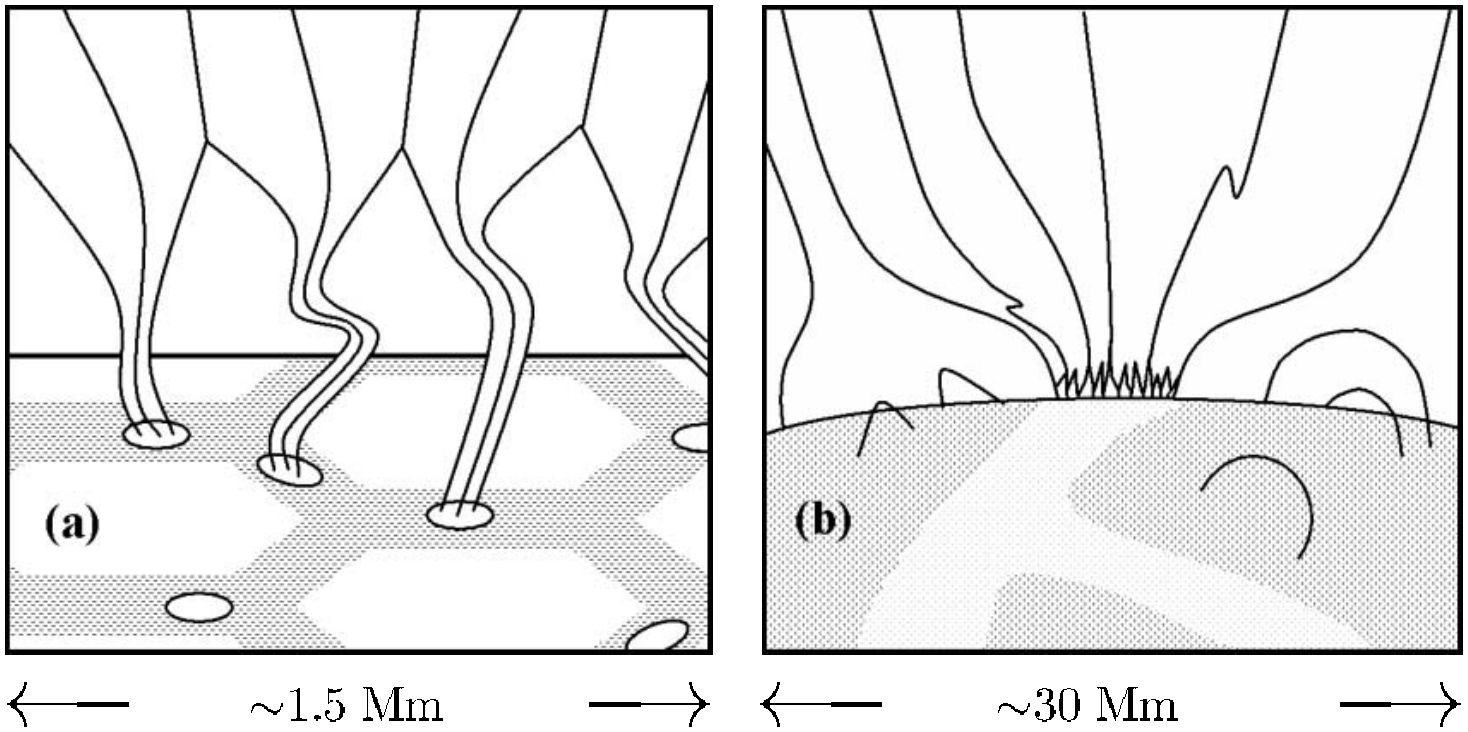
\includegraphics[width=0.6\textwidth]{figures_of_others/images/Cranmer2005_fig1_ab.png}
	}{
		\caption[\lofimage{figures_of_others/images/Cranmer2005_fig1_ab.png}Credit: {\citet[Fig.~1, panels (a) and (b)]{Cranmer2005}}, \textcopyright~AAS, reproduced with permission.]
		{Schemata of superradially expanding magnetic flux. (a) magnetic bright points between granules on the photosphere are indicated by ellipses. The protruding lines are thin magnetic flux tubes that merge to a homogeneous network field. (b) Pictured is the network field which expands again to the large-scale canopy field of the lower corona. Credit: {\citet[Fig.~1, panels (a) and (b)]{Cranmer2005}}, \textcopyright~AAS, reproduced with permission.}
		\label{fig:Cranmer2005_fig1_ab}
	}
	\addtocontents{lof}{\smallskip\protect\center See the following email correspondence.\medskip
		\protect\lstinputlisting{figures_of_others/permissions/Cranmer2005_fig1_IOP_permission.txt}
		The related email attachment:
		\protect\lstinputlisting{figures_of_others/permissions/Cranmer2005_fig1_permission.txt}
	}
\end{figure}

%%% Alfvén waves
The magnetic bright points' convective appearance and stochastic motions on the photosphere result in wavelike fluctuations that propagate upward through the superradially expanding flux tubes. There exist three types of magnetohydrodynamic (MHD) waves within the plasma: compressional fast- and slow-mode waves, and an incompressible wave mode, which is the result of bending magnetic field lines \citep{Alfven1942}, called shear Alfvén wave. Alfvén waves propagate with a characteristic speed along magnetic field lines. As they transport energy from the photosphere outwards, it is assumed that they play a major role in the coronal heating process and that the solar wind is accelerated up to the so-called Alfvén critical surface at around \SI{17}{\Rs}, where the local Alfvén speed equals the solar wind speed \citep{Sittler1999,Exarhos2000}. Alfvén waves are dominant in coronal regions that have open magnetic field lines, that is, coronal holes, and thus they leak into the fast solar wind \citep{Cranmer2005}. Within solar wind at \SI{1}{\au}, their average velocity is about \SI{57}{\km\per\s} \citep{Veselovsky2010} -- for more details about the Alfvén velocity see Appendix~\ref{sec:alfvén_velocity}.

%%% field geometry from source surface on to heliopause
The plasma in open coronal regions expands superradially, following the magnetic field lines. However, the field strength decreases with increasing solar distance and at a distance of about \SI{2.5}{\Rs} the thermal pressure becomes larger than the magnetic pressure. Thereby the magnetic field gets frozen within the plasma and is carried by the solar wind radially outwards into the heliosphere. The distance from which the solar wind propagation gets released from the magnetic field lines is called the source surface \citep{Schatten1969} and the thermal to magnetic pressure ratio is termed plasma beta -- for more details on plasma beta see Appendix~\ref{sec:plasma_beta}. The magnetic field changes from superradial expansion below the source surface to a radial configuration above it, this field geometry is also visible in the total eclipse image in \autoref{fig:Tse2008_500_mo1}.

%%% heliospheric current sheet
Open field lines expand over adjacent closed field regions. Above the cusps of these regions' closed loops, the surrounding plasma flows encounter each other and stream outwards, forming so-called helmet streamers. Above these helmet streamers, magnetic boundaries are created by plasma flows, carrying opposite magnetic polarity. These boundaries constitute an extensive coronal neutral line around the Sun. Within the heliosphere, the two dominating magnetic polarity regions, originating from both solar magnetic poles, are separated by the extension of this neutral line: a large plasma boundary surface, termed the heliospheric current sheet (HCS) \citep{Smith2001}.

In the quiet Sun during solar cycle minimum conditions, coronal holes are the main photospheric sources of the heliospheric magnetic field. The magnetic dipole axis is then near the rotation axis and thus the HCS is roughly located near the equatorial plane, dividing both hemispheres. The analytical solar magnetic field model for solar minimum conditions, constructed by \citet{Banaszkiewicz1998}, shows this field geometry as seen in \autoref{fig:Banaszkiewicz1998_DQCS_model_raw}. The quadrupole part of their dipole plus quadrupole plus current sheet (DQCS) model considers the closed equatorial fields and allows equatorial outflow along the current sheet.
\begin{figure}[htb]
	\begin{floatrow}
		\ffigbox{
			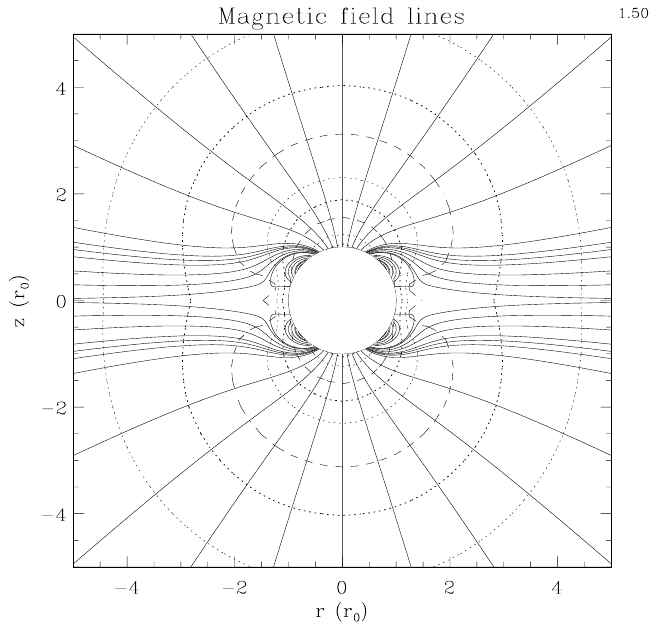
\includegraphics[width=0.46\textwidth]{figures_of_others/images/Banaszkiewicz1998_DQCS_model_raw.png}
		}{
			\caption[\lofimage{figures_of_others/images/Banaszkiewicz1998_DQCS_model_raw.png}Credit: {\citet[Fig.~3]{Banaszkiewicz1998}}, \textcopyright~ESO, reproduced with permission.]
			{Model of the solar magnetic field geometry in the polar plane for solar cycle minimum. Magnetic field lines (solid) and constant field strength surfaces (dashed) from the DQCS model are plotted. The field line spacing does not represent the field strength but provides better detail where needed. Credit: {\citet[Fig.~3]{Banaszkiewicz1998}}, \textcopyright~ESO, reproduced with permission.}
			\label{fig:Banaszkiewicz1998_DQCS_model_raw}
		}
		\addtocontents{lof}{\smallskip\protect\center See the following document.\protect\\
			\protect\fbox{\protect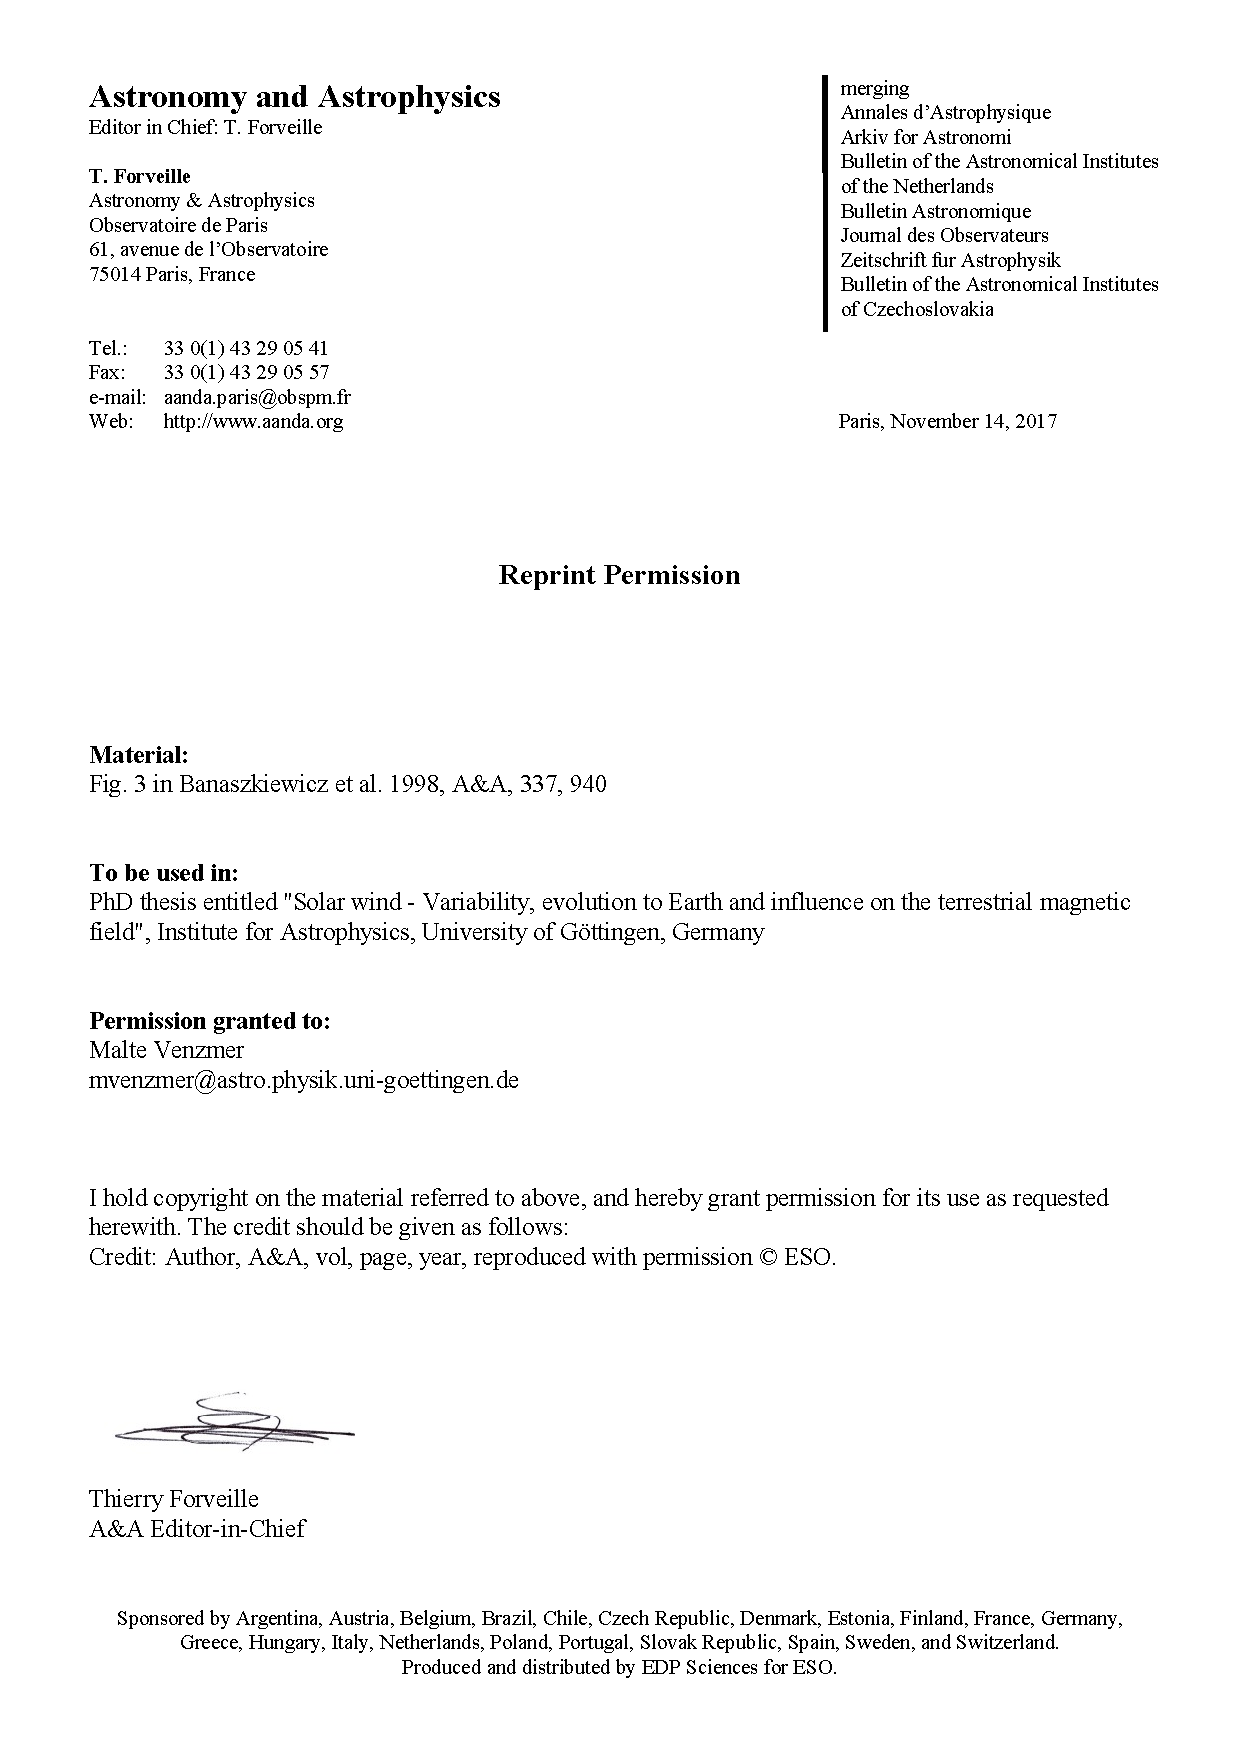
\includegraphics[width=0.6\textwidth,angle=90]{figures_of_others/permissions/permission_request_Banaszkiewicz1998_fig3.pdf}}
			\medskip
		}
		\ffigbox{
			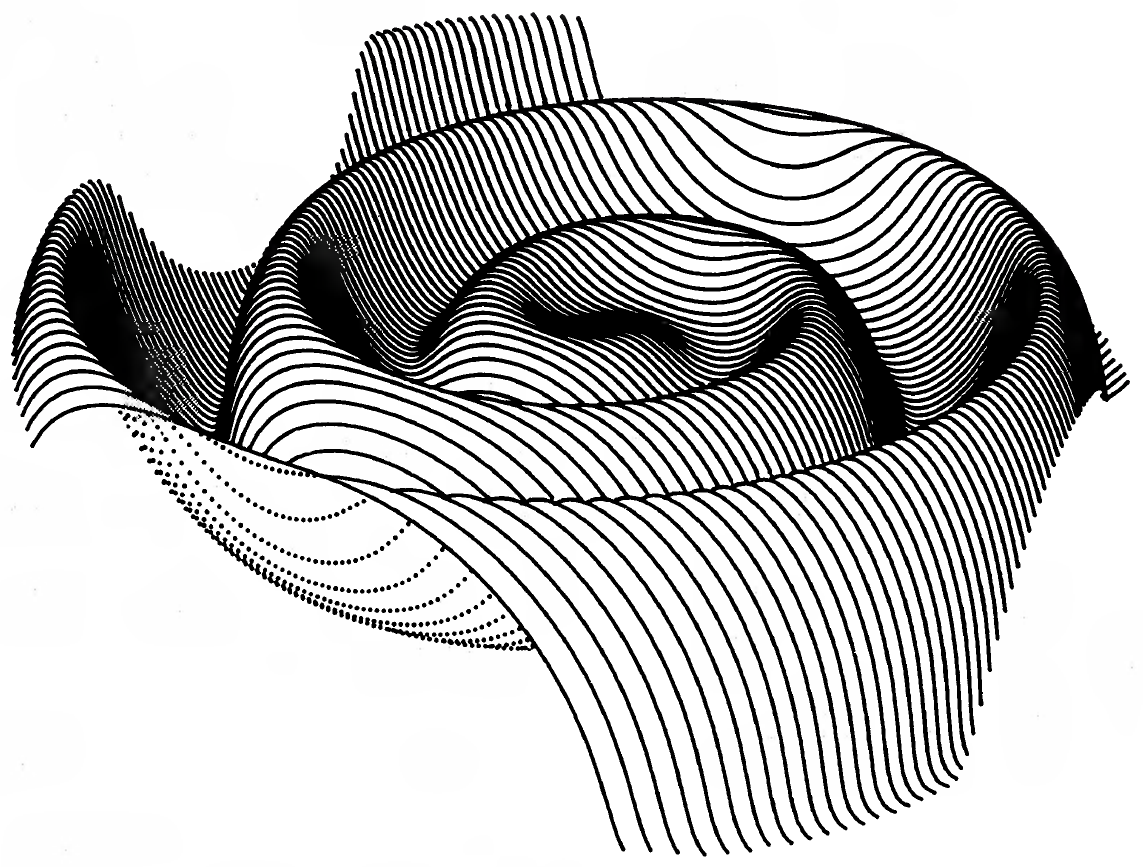
\includegraphics[width=\Xhsize]{figures_of_others/images/Jokipii1981_ballerina_HCS.png}
		}{
			\caption[\lofimage{figures_of_others/images/Jokipii1981_ballerina_HCS.png}Credit: {\citep[Fig.~2]{Jokipii1981}}, \textcopyright~AAS, reproduced with permission.]
			{A simple HCS model, where its wavy surface shape solely stems from a solar dipole tilt of \SI{15}{\degree} to the rotation axis. The figure's extend is \SI{25}{\au} across. Credit: {\citep[Fig.~2]{Jokipii1981}}, \textcopyright~AAS, reproduced with permission.}
			\label{fig:Jokipii1981_ballerina_HCS}
		}
		\addtocontents{lof}{\smallskip\protect\center See the following email correspondence.\medskip
			\protect\lstinputlisting{figures_of_others/permissions/Jokipii1981_permission.txt}
		}
	\end{floatrow}
\end{figure}
Around solar minimum, the HCS's warped surface typically looks like a wavy ballerina skirt, due to the varying tilt angle between the dipole axis and the rotation axis, see \autoref{fig:Jokipii1981_ballerina_HCS}, and also due to local magnetic field variations \citep{Jokipii1981}.

During the field transition at solar maximum, the dipole axis shifts to lower latitudes, crosses the solar equator, and eventually the field ends up in a reversed dipole configuration \citep{Jones2003}. During this process, the HCS rotates almost rigidly together with the dipole axis and remains a single connected structure in the inner heliosphere \citep{Jones2003}. Hence during cycle maximum, the HCS has a very complex shape, is largely inclined to the solar equator, and reaches near-polar latitudes.

%%% Parker spiral
The solar wind source surface rotates with the Sun and thus shears the HMF into an Archimedean spiral pattern, adding an azimuthal component to the radial HMF. This geometry was anticipated by \citet{Parker1958} and is today called Parker spiral. The Parker spiral, viewed in the ecliptic plane, is illustrated in \autoref{fig:Owens2013_PFSS_Sectors_screenshot}. The solar rotation axis tilt of up to \SI{7.25}{\degree} to the ecliptic leads to a slight diving into both hemispheres of opposite polarity. Thus, together with the ballerina topology of the HCS, the Parker spiral has typically a structure of either two or four sectors of alternating magnetic polarity \citep{Ness1965}, which are separated by the HCS.

%other magnetic structures
The just described HMF geometry is also overlaid by other magnetic structures than the HCS. Speed differences between solar wind streams, and between solar wind and CMEs cause enhanced field amplitudes and can result in shocks in the HMF. Furthermore, CMEs in the solar wind carry magnetic clouds (MCs) and their frequency and magnetic configuration vary with the solar activity cycle. These solar wind and CME structures are described in more detail in the following sections.

%%% out to heliopause
That way, the magnetic field and its structures are carried out to the termination shock by the solar wind. MHD simulations, based on in-situ measurements of Voyager~1 and 2 within the heliosheath and based on IBEX observations of energetic neutral atoms, provide indications about the outer structure of the heliosheath. Behind the termination shock, the magnetic sector boundaries are compressed and they reconnect, forming magnetic bubbles \citep{Opher2011}. These bubbles -- unconnected to the HMF -- flow away to the heliosheath tail region. Even beyond the termination shock, the solar wind plasma seems confined and collimated by the twisted solar magnetic field and driven into a northern and a southern jet \citep{Opher2015}. Hence, the Sun's magnetosphere has likely a croissant-like shape with two turbulent tail-lobes, where eventually the solar wind and the HMF are being mixed into the interstellar medium.

\clearpage

\begin{figure}[htb]
	\fcapside[\FBwidth]{
		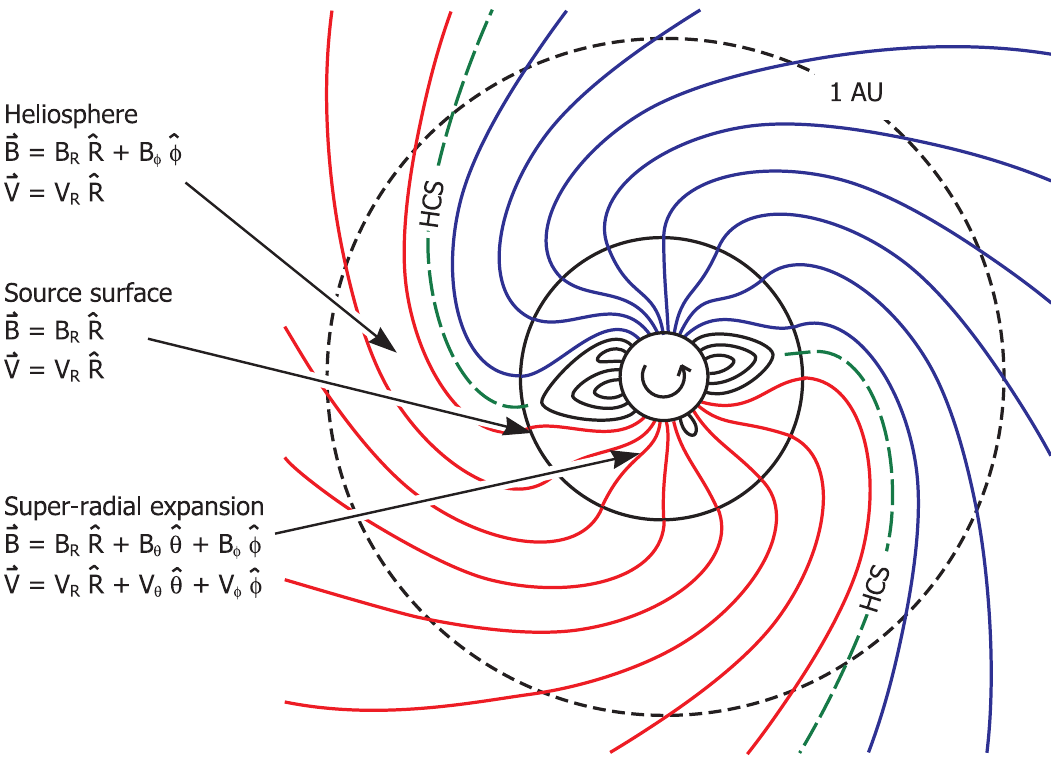
\includegraphics[width=0.6\textwidth]{figures_of_others/images/Owens2013_PFSS_Sectors_screenshot.png}
	}{
		\caption[\lofimage{figures_of_others/images/Owens2013_PFSS_Sectors_screenshot.png}Credit: {\citet[Fig.~1]{Owens2013}}, adapted from {\citet[Fig.~1]{Schatten1969}}, licensed under \href{https://creativecommons.org/licenses/by-nc/3.0/de/}{CC BY-NC 3.0 DE}.]
		{Illustration of the Parker spiral formation in the ecliptic plane outside the source surface. The HCS (green) is located between solar wind flows of opposite magnetic field polarity (red/blue). Credit: {\citet[Fig.~1]{Owens2013}}, adapted from {\citet[Fig.~1]{Schatten1969}}, licensed under \href{https://creativecommons.org/licenses/by-nc/3.0/de/}{CC BY-NC 3.0 DE}.}
		\label{fig:Owens2013_PFSS_Sectors_screenshot}
		%Owens2013 figure permission request: open access article
	}
	\addtocontents{lof}{\smallskip\protect\center See the permission to \autoref{fig:Owens2013_Heliosphere_screenshot}.\medskip}
\end{figure}


\section{Solar wind}
\label{sec:solar_wind}
%%% sw history
It is observed that cometary ion tails point away from the Sun and lag only a few degrees from the radial direction, sometimes they also show fluctuations and become kinked. As such behavior could not be explained by interaction with sunlight pressure, eventually \citet{Biermann1951} concluded that cometary ion tails are influenced by a continuous flow of particles from the Sun.	%Kivelson1995, p14+91
\citet{Parker1958} considered the consequences of Biermann's conclusions and built a solar wind model, adopting an expanding isothermal solar atmosphere. Parker also incorporated the implications for the solar magnetic field in his model and hence he laid the theoretical foundations for a continuous supersonic radial outflow of magnetized plasma. Thus, the existence of the solar wind was postulated before the first satellites measured it in~situ in 1959 \citep{Gringauz1960,Neugebauer1966}. Since that time, spacecraft are able to measure the solar wind almost continuously with magnetometer and plasma instruments in~situ (see \autoref{chap:data}). Pronounced solar wind structures, such as CMEs and streamers, become visible with the use of space-based coronagraph imagers. From Earth, the near-Sun outflow geometry of solar wind can be observed only during solar eclipses, see the eclipse photo in \autoref{fig:Tse2008_500_mo1}.

%%% plasma composition, parameter ranges and properties
The solar wind is a magnetized plasma consisting of electrons and ions. The ions are mainly composed of hydrogen, a small percentage of helium, and traces of oxygen, carbon, and other metals. The average abundance of helium is about \SI{4.5}{\%} and in slow wind at solar cycle minimum conditions less than \SI{2}{\%} \citep{Feldman1978,Schwenn1983,Kasper2012}.
The solar wind is commonly approximated by an ideal incompressible MHD plasma (viscosity $\mu = 0$ and electrical conductivity $\sigma = \infty$) and can be viewed as a neutral plasma. Also, its helium share is often viewed as being constant, in this case the proton density determines both the helium and electron densities.

The properties of solar wind are highly variable in time and space. The key properties are determined by the values of the solar wind parameters magnetic field strength, proton velocity, density, and temperature. Their average magnitudes scale with solar activity, heliographic latitude, and solar distance. At the solar distance of Earth however, most of the time these parameters' typical values lie in the ranges \SIrange{3}{8}{\nano\tesla}, \SIrange{300}{500}{\km\per\s}, \SIrange{2}{8}{\per\cm\cubed}, and \SIrange{e4}{e5}{\K} (\citealp[p.~92]{Kivelson1995}; \citealt{Venzmer2018}). The low density of solar wind can be illustrated with a short comparison: 1~liter of air at standard pressure, expanded to a typical solar wind density of \SI{6.5}{\per\cm\cubed}, would occupy a volume of a cube with edge length of about \SI{155}{\km}.
% sw density considerations:\\
% 1 mol approx 24.7895 l/mol at 25 °C and 1 bar
% Avogadro constant N_A = 6.022140857(74)e23 mol−1
% 1 liter air @ 1 bar equates to 1/24.7895 mol = 2.4293e+22
% 2.4293e+22 / 6.5 cm-3 = 3.7374e+21 cm3 = 3.7374e6 km3 = (155 km)3
% 1 liter air @ 1 bar (need 24 ms for passing 1 dm2 area @ 15 km/h)\\
% equals\\
% 3.7e6 km3 = (155 km)3 solar wind @ 6.5 cm-3 (need 43900 a for passing 1 dm2 area @ 400 km/s)\\
Solar wind quantities, such as particle flux densities, mass flux, pressures, and plasma beta, can be derived from the four listed parameters. Having the parameters in the aforementioned ranges, the solar wind is a plasma with a beta mostly greater than unity, that is, the average solar wind carries the magnetic field and its motions are not influenced by the field direction (for more on plasma beta see Appendix~\ref{sec:plasma_beta}).
% mean beta: 1.714\\	%from mean paper values
% low beta: 0.180\\	%from ranges above
% high beta: 8.444\\	%from ranges above

However, solar wind is structured by its different sources in the solar corona. It consists of fast continuous streams, slow variable flows, and transient CME events. These different flows have highly variable velocities, which result in compressed or rarefied regions at their interfaces. Additionally, the source region's magnetic field configuration organizes the interplanetary magnetic field (IMF), transported within the solar wind plasma. Regardless, pronounced magnetic structures embedded in the solar wind, such as field polarity changes or magnetic clouds, still influence the properties of the plasma.

\pagebreak

This multitude of structures is apparent in the two months -- beginning in May~2013 -- of in-situ measured solar wind, which I present as an example period in \autoref{fig:ACE_64s_v7_thesis_CIRs_2013-5-1_65_plot}.
\begin{figure}[t]
	\centering
	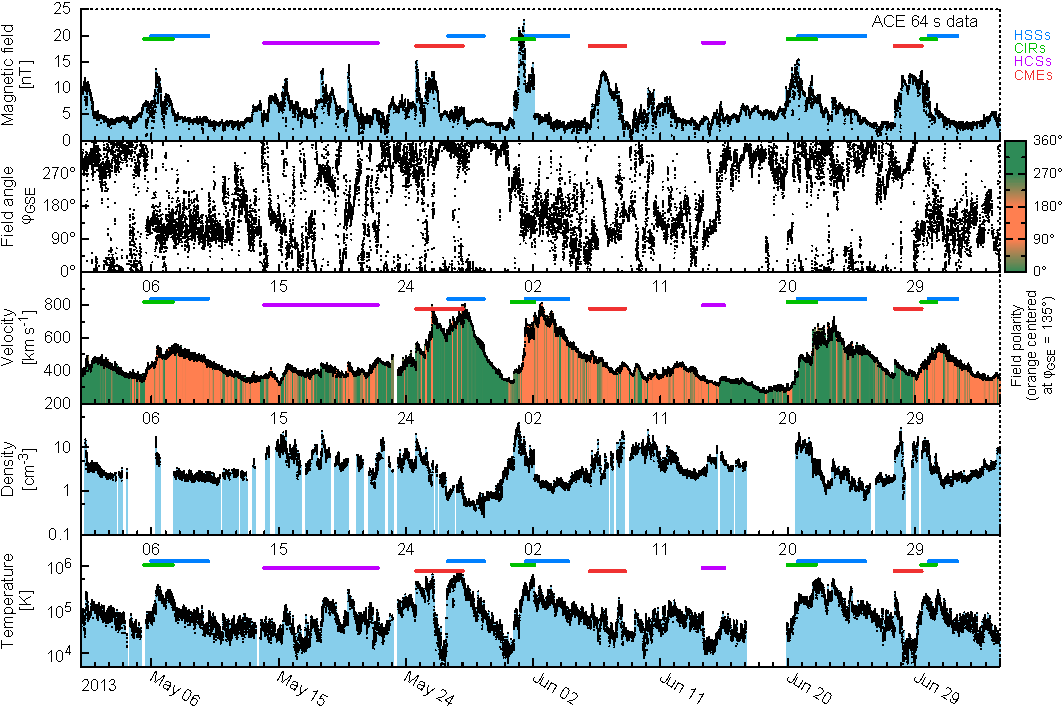
\includegraphics[width=\textwidth]{figures_of_mine/gnuplots/ACE_64s_v7_thesis_CIRs_2013-5-1_65_plot.pdf}
	\caption[\lofimage{figures_of_mine/gnuplots/ACE_64s_v7_thesis_CIRs_2013-5-1_65_plot.pdf}I created the figure myself.]
	{Solar wind with several structures, measured at L1 during the time period 1~May to 5~July in 2013. The parameters are the magnetic field strength, its field angle in the ecliptic in GSE~coordinates, the proton velocity, density, and temperature. I indicated periods of prominent solar wind structures with color bars: HSSs in blue, CIRs in green, HCSs in purple, and CMEs in red. In the velocity panel also the field polarity is color coded -- assuming a Parker spiral angle of \SI{135}{\degree} at L1. Blank periods indicate bad or missing data. The data are 64~s measurements from the ACE spacecraft.}
	\label{fig:ACE_64s_v7_thesis_CIRs_2013-5-1_65_plot}
% 	\addtocontents{lof}{\smallskip\protect\center I created the figure myself.\medskip}
\end{figure}
The IMF and solar wind ion parameters were measured with the MAG and SWEPAM instruments on board the Advanced Composition Explorer (ACE) spacecraft, located around the first Lagrange point (L1). The data have a time resolution of 64~seconds and are obtained from the ACE~Science~Center web interface\footnote{ACE Science Center website: \urlfoot{http://www.srl.caltech.edu/ACE/ASC/}}.

Some general solar wind tendencies can be seen from this plot: The temperature of the solar wind scales with its stream velocity; compressed plasma regions enhance the magnetic field and the density; HCSs, magnetic sector boundaries, and MCs come with high densities and low temperatures; MCs in CMEs have high magnetic fields and low temperatures. I indicated the periods of occurring solar wind structures, that is, HSSs, CIRs, HCSs, and CMEs, with colored bars -- these types are further described in the following sections.


\subsection{Slow and fast streams}
\label{sec:slow_and_fast_streams}
%%% fast and slow solar wind
It is observed at \SI{1}{\au} that the continuous solar wind comes in streams roughly focused at two major velocity ranges \citep{Neugebauer1966,Schwenn1983}, slow and fast streams with \SIrange{250}{450}{\km\per\s} and \SIrange{450}{800}{\km\per\s} respectively. Both types possess differences in their typical characteristics and ion compositions. Apart from its higher speeds, fast solar wind has most prominently lower proton densities ($\sim$\,\SI{3}{\per\cm\cubed}) and higher temperatures ($\sim$\,\SI{2e5}{\K}) than the slow solar wind, which has higher densities ($\sim$\,\SI{10}{\per\cm\cubed}) and lower temperatures ($\sim$\,\SI{4e4}{\K}) \citep{Schwenn1990}. The fast solar wind has a nature of coming in steady high-speed streams (HSSs) with a unique magnetic field polarity, whereas slow solar wind is much more variable in all its properties except its velocity \citep{Bame1977}. HSSs are further overlaid with Alfvén waves, which modulate the stream velocity with typical periods of \SIrange{15}{60}{\minute}.

%sources of fast wind
First soft X-ray observations of the corona, made during sounding rocket flights in the early 1970s, showed clearly that the fast solar wind emerges from extended areas of reduced X-ray emission, subsequently called coronal holes (CHs) \citep{Krieger1973,Hundhausen1977}. A small equatorial CH, located near the center of the solar disk, is shown in the SDO/AIA image taken on 29~May 2013, see \autoref{fig:20130529_000119_1024_0193}. This particular CH is most likely responsible for the HSS observed at L1 on 1--5~June 2013, visible in the previous solar wind plot in \autoref{fig:ACE_64s_v7_thesis_CIRs_2013-5-1_65_plot}.
\begin{figure}[t]
	\begin{floatrow}
		\ffigbox{
			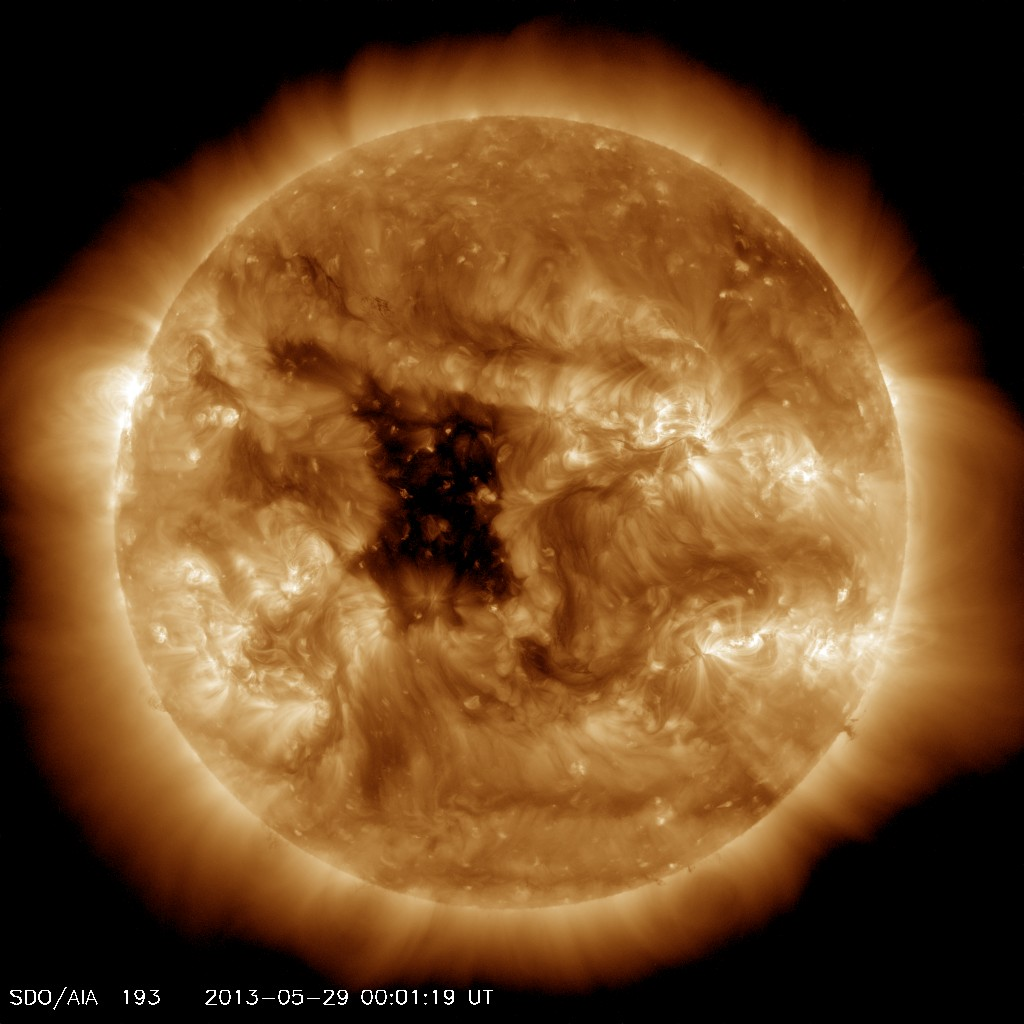
\includegraphics[width=0.46\textwidth]{figures_of_others/images/20130529_000119_1024_0193.jpg}
		}{
			\caption[\lofimage{figures_of_others/images/20130529_000119_1024_0193.jpg}Credit: NASA/SDO and the AIA, EVE and HMI science teams.]
			{Image of the solar corona during solar cycle maximum from 29~May 2013, seen in a wavelength of \SI{193}{\angstrom}. The dark area near the center of the solar disk is an equatorial CH, typical for high solar activity conditions. Credit: NASA/SDO and the AIA, EVE and HMI science teams.}
			\label{fig:20130529_000119_1024_0193}
		}
		\ffigbox{
			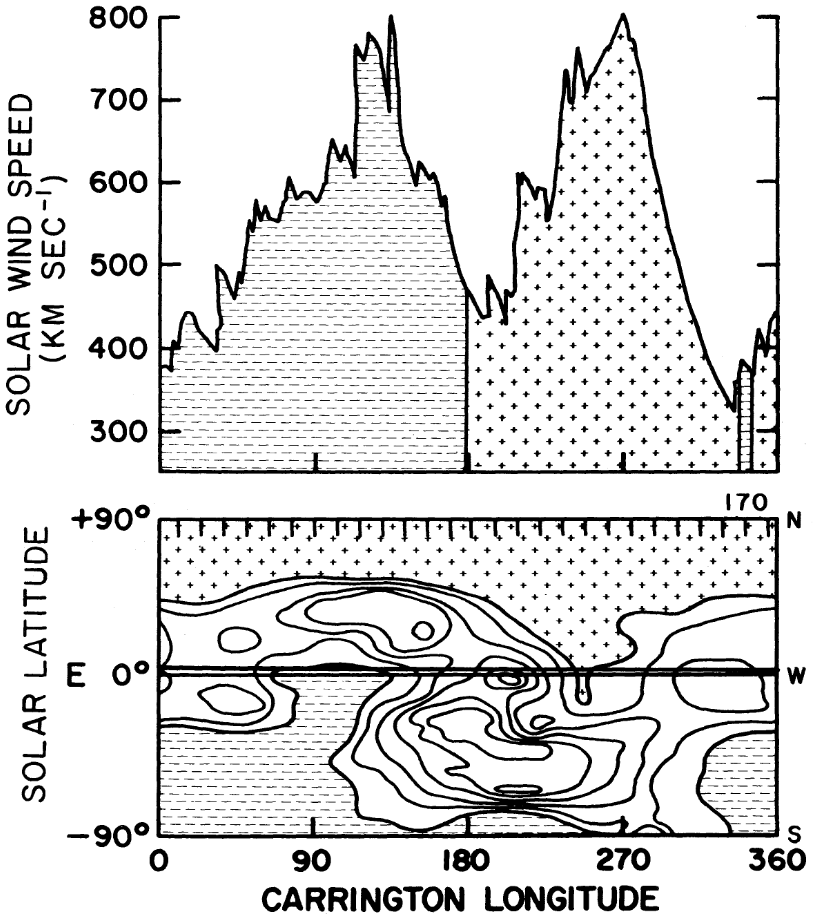
\includegraphics[width=0.85\Xhsize]{figures_of_others/images/Hundhausen1977_fig10_cut.png}
		}{
			\caption[\lofimage{figures_of_others/images/Hundhausen1977_fig10_cut.png}Credit: {\citet[Fig.~10]{Hundhausen1977}}, \textcopyright~Colorado Associated University Press, reproduced with permission.]
			{Solar wind velocity with respect to its estimated source longitude (top) and coronal brightness contour map at \SI{0.5}{\Rs} above the photosphere (bottom) for the Carrington rotation 1616. The velocity is based on IMP spacecraft data, back-extrapolated to \SI{20}{\Rs}. Brightness values below a fixed threshold are shaded corresponding to the magnetic field polarity ($+$/$-$) of the underlying photosphere. The map is based on observations from the K-coronameter at the Manua~Loa Observatory. Credit: {\citet[Fig.~10]{Hundhausen1977}}, \textcopyright~Colorado Associated University Press, reproduced with permission.}
			\label{fig:Hundhausen1977_fig10_cut}
		}
		\addtocontents{lof}{\smallskip\protect\center additional permission for publishing pending...\medskip}
	\end{floatrow}
\end{figure}
The magnetic field polarities found in CHs are associated with the magnetic field directions observed in HSSs, as seen in \autoref{fig:Hundhausen1977_fig10_cut}. In coronal regions with closed magnetic field lines, the plasma is trapped, though in CHs it can escape, following the open magnetic field lines outwards into space. Wave-particle interactions heat and accelerate the ions in CHs, likely leading to the emission of the fast solar wind \citep{Hollweg2002}. Superradial expansion of the magnetic field lines in the corona has an influence on the wind speed -- actually the expansion factor is anticorrelated with the final wind velocity \citep{Wang1990}. As the field expansion is larger near the border of CHs, faster wind emerges from the mid regions of CHs, forming into HSSs. However, there are indications that the slow and fast solar wind are not only generated at different sources but from distinct mechanisms \citep{McGregor2011b}.

%sources of slow solar wind
The high variability in the slow solar wind points to the existence of different types of slow wind flows, originating from separate coronal locations and mechanisms \citep{Schwenn1983}. It is still under debate if the variability is produced by the formation mechanism of the slow solar wind or if the variability is caused during the acceleration/propagation phase \citep{Sanchez-Diaz2016}. Still, at least a part of its variability can be attributed to the interactions between slow and fast solar wind, which result in a general reduction in velocity differences and thus let solar winds of different speeds (having different properties as well) converge to a common intermediate speed regime in the range \SIrange{400}{500}{\km\per\s} \citep{McGregor2011a,Sanchez-Diaz2016}. Studies using remote white-light tracing of coronal material and in-situ measurements of solar wind suggest that multiple sources of slow solar wind flows exist \citep{Wang2000,Kilpua2016}. To the best of my knowledge, the generally considered sources are listed in the following:
\begin{itemize*}
	\item CH boundaries and small CHs, because their plasma outflow is slower due to the high superradial expansion of its open field lines \citep{Wang1990}.
	\item CH boundaries, when trapped plasma is released by reconnection between open and closed field lines \citep{Madjarska2004}.
	\item Helmet/pseudo-streamers in active regions, where transient plasma blobs are released from the cusps of closed field loops \citep{Wang1998,Wang2000}. This slow and dense material is associated with the heliospheric plasma sheet belt.
	\item Edges of active regions, which have hot plasma outflows with a single magnetic polarity \citep{Kojima1999}.
	\item Jets originating from coronal bright points might contribute to the slow solar wind \citep{Subramanian2010}.
	\item Slow unidentified CMEs can contribute to slow wind observations as well, as noted by \citet{Wang2000}.
\end{itemize*}
% Kilpua2016 generally suggested sources:\\
% - CH boundaries, the plasma is slow due to superradial expansion of open field lines\\
% - transient plasma blobs that are released from the helmet/pseudo-streamers\\
% - plasma released by reconnection between open and closed field lines at the coronal hole boundaries\\
% - hot outflows with speeds up to ∼100~km/s from the edges of active regions, first reported by Kojima1999\\
% - jets originating from coronal bright points\\

It is found to be difficult to use in-situ measurements for tracing the slow solar wind flow types to different origins and to distinguish between them, because most properties are also highly variable in time \citep{Kilpua2016}. However, some indicators show tendencies to differentiate between the slow winds from different source regions. Notable indicators are: elemental ion ratios, heavy ion charge states, and the specific entropy.

The elemental composition of the coronal plasma varies with height/location in the solar atmosphere, therefore the solar wind's elemental ion ratios (e.g., $\text{He}/\text{H}$, $\text{Fe}/\text{O}$) are used to determine its origin.
The charge states of coronal heavy ions depend on the local temperature. However, the density of the outwards expanding plasma decreases fast, preventing further ionization/recombination. The charge states decouple from the local temperature and freeze~in close to the Sun. Thus, heavy ion charge ratios (e.g., $\text{C}^{+6}\!/\text{C}^{+4}$, $\text{O}^{+7}\!/\text{O}^{+6}$) in the solar wind track the coronal source temperature and especially the $\text{C}^{+6}\!/\text{C}^{+4}$ ratio is sensitive to the solar wind type \citep{Landi2012}.
At solar minimum the specific proton entropy is found to correlate with the $\text{O}^{+7}\!/\text{O}^{+6}$ ratio and thus able to trace slow solar wind sources as well \citep{Pagel2004}.
%specific entropy: $\ln\left(T_\text{p}/n_\text{p}^{\gamma - 1}\right)$ ($\gamma = 1.5$)

%solar activity dependence
The solar wind stream pattern varies strongly with solar activity. The Sun's ordered dipole structure during solar cycle minima leads to polar regions with open magnetic fields, constituting large coronal holes, and to a large equatorial belt region with closed magnetic fields -- this is clearly visible in Figures~\ref{fig:Tse2008_500_mo1} and \ref{fig:Banaszkiewicz1998_DQCS_model_raw}. This state results in fast solar wind coming exclusively from the poles and higher latitudes, whereas active regions form an equatorial streamer belt around the Sun, emitting slow solar wind. This structure was confirmed from solar wind speed measurements done by the Ulysses spacecraft, which flew in an out-of-ecliptic solar orbit and whose mission covered a duration of more than one solar cycle \citep{McComas200809}, see \autoref{fig:McComas2008_Ulysses_orbit}.
\begin{figure}[htb]
	\centering
	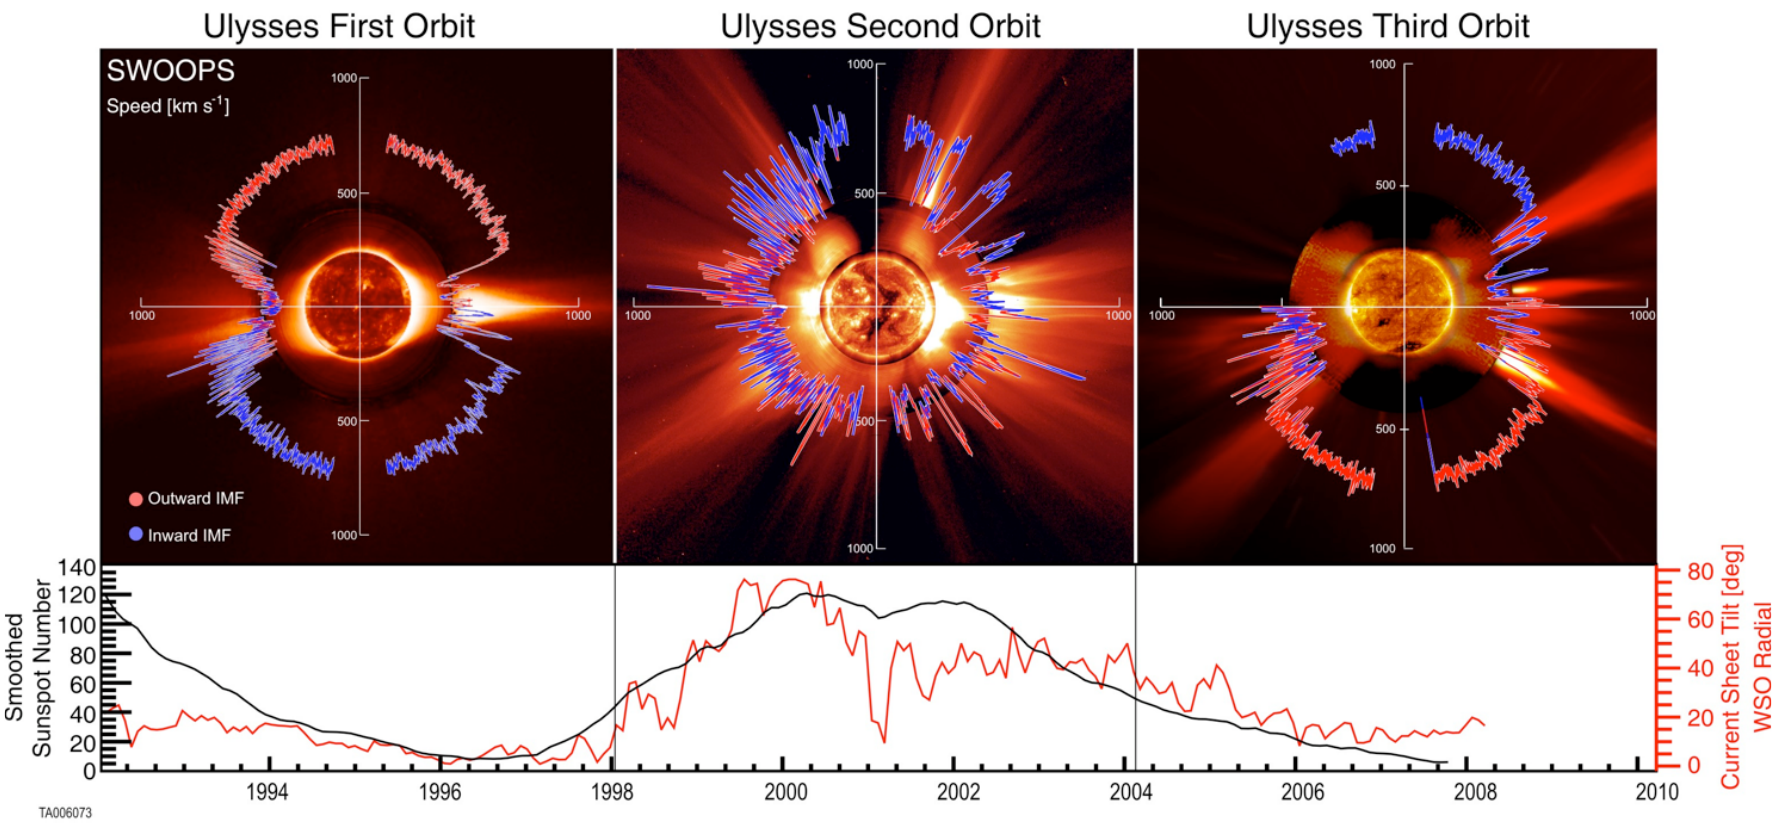
\includegraphics[width=\textwidth]{figures_of_others/images/McComas2008_Ulysses_orbit_.png}
	\caption[\lofimage{figures_of_others/images/McComas2008_Ulysses_orbit_.png}Credit: {\citet[Fig.~1]{McComas200809}}, \textcopyright~American Geophysical Union, reproduced with permission.]
	{Solar wind velocity and magnetic field polarity (red/blue) with respect to heliographic latitude for the three orbits of the Ulysses spacecraft during low and high solar activity (upper panels). The data starts top left and runs couterclockwise. The corresponding smoothed SSN (black) and HCS tilt angle (red) are plotted beneath. The background consists of solar images for solar cycle~22 minimum (1996-08-17), solar cycle~23 maximum (2000-07-12), and solar cycle~23 minimum (2006-03-28). The solar disk, inner corona, and outer corona images are from SOHO/EIT (Fe~XII at \SI{1950}{\nano\meter}), Mauna~Loa K~coronameter (\SIrange{700}{950}{\nano\meter}), and SOHO/C2 white light coronagraph. Credit: {\citet[Fig.~1]{McComas200809}}, \textcopyright~American Geophysical Union, reproduced with permission.}
	\label{fig:McComas2008_Ulysses_orbit}
	\addtocontents{lof}{\smallskip\protect\center See the document on the next page.
		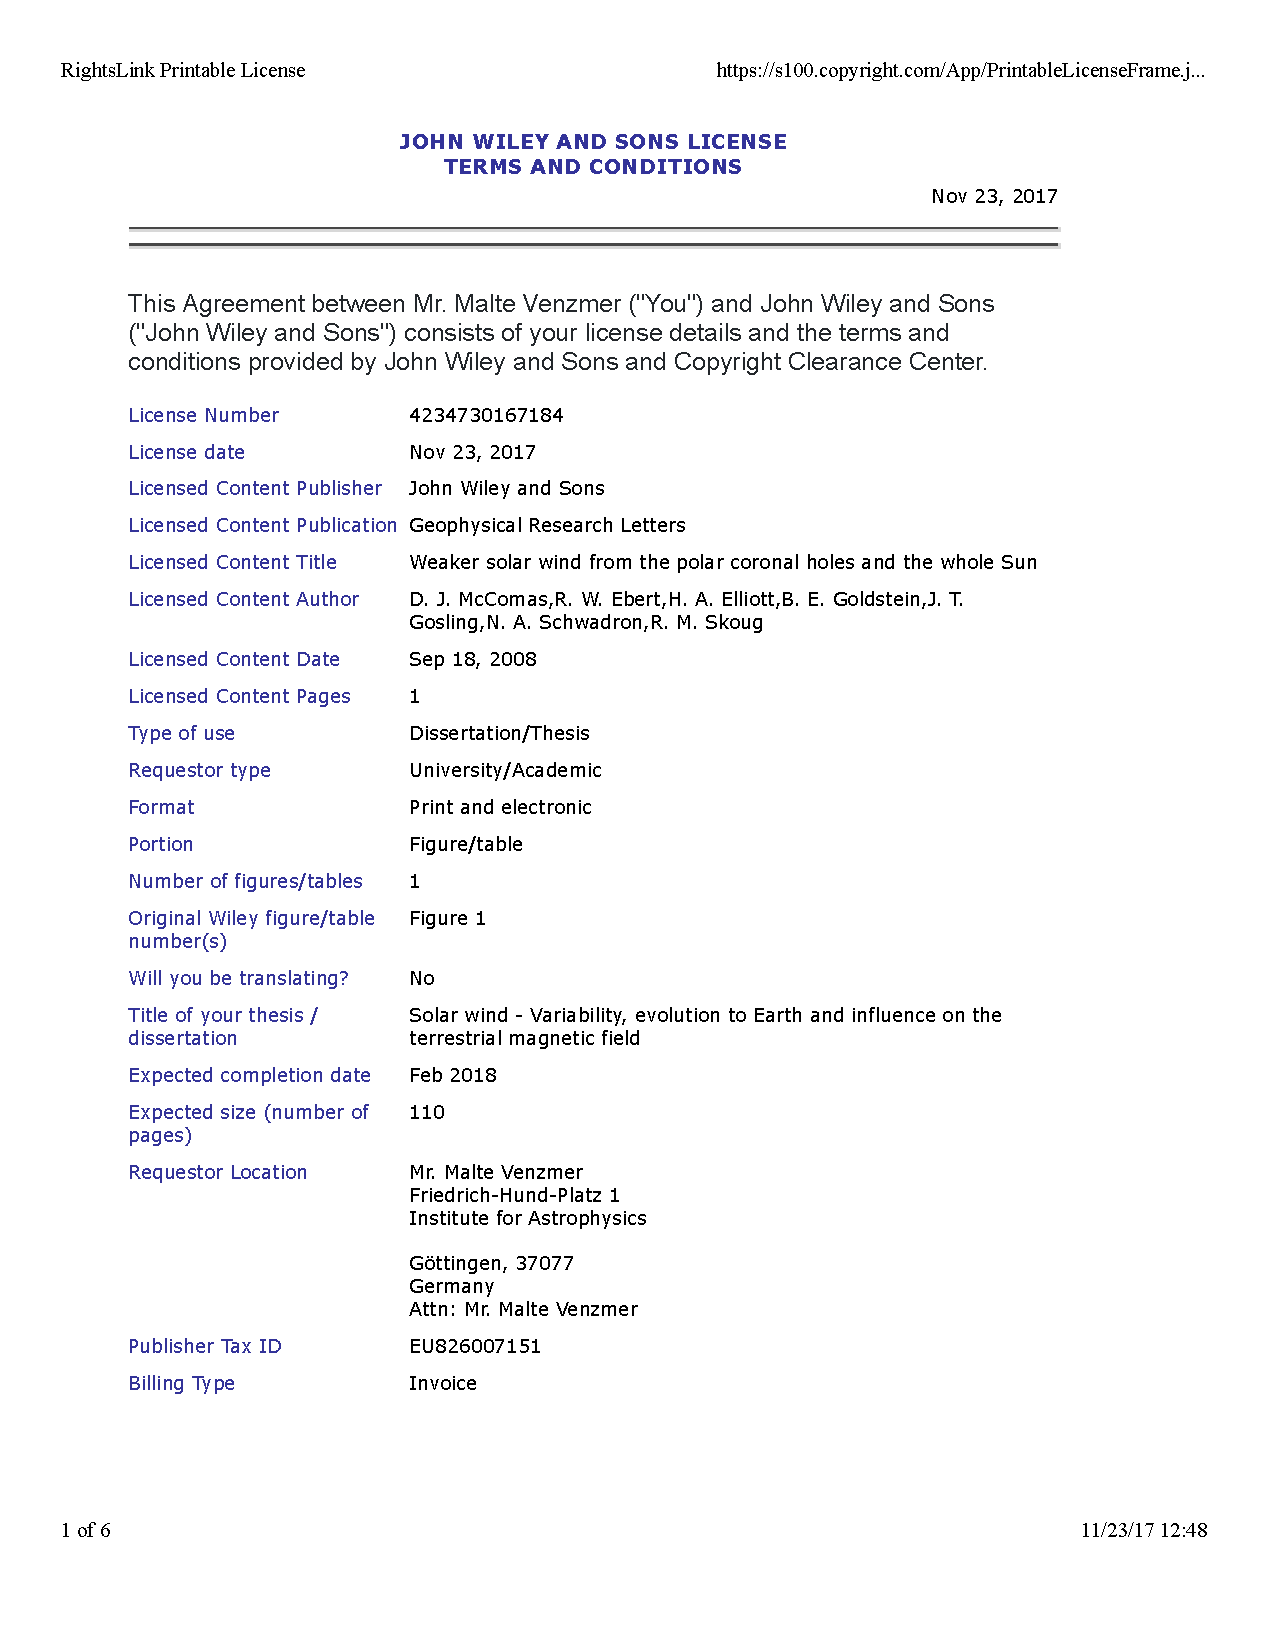
\includepdf[pages={-},nup=2x3,delta=1cm 2mm,column=true,frame=true,noautoscale=true,scale=0.32]{figures_of_others/permissions/permission_request_McComas2008a_fig1.pdf}
	}
\end{figure}
%figure source: http://onlinelibrary.wiley.com/doi/10.1029/2003GL017136/full
%McComas200809: (a–c) Polar plots of the solar wind speed, colored by IMF polarity for Ulysses' three polar orbits colored to indicate measured magnetic polarity. In each, the earliest times are on the left (nine o'clock position) and progress around counterclockwise. (d) Contemporaneous values for the smoothed sunspot number (black) and heliospheric current sheet tilt (red), lined up to match Figures 1a–1c. In Figures 1a–1c, the solar wind speed is plotted over characteristic solar images for solar minimum for cycle 22 (8/17/96), solar maximum for cycle 23 (12/07/00), and solar minimum for cycle 23 (03/28/06). From the center out, we blend images from the Solar and Heliospheric Observatory (SOHO) Extreme ultraviolet Imaging Telescope (Fe XII at 1950 nm), the Mauna Loa K coronameter (700–950 nm), and the SOHO C2 white light coronagraph.
The transition of the solar magnetic field during the solar cycle maxima induces the chaotic appearance of closed magnetic fields at higher latitudes and even near the poles. Furthermore, coronal holes begin to invade parts of the equatorial region, leading to recurring phases of HSSs in the ecliptic. This can be seen from the solar wind period in \autoref{fig:ACE_64s_v7_thesis_CIRs_2013-5-1_65_plot}, where recurrent HSSs of the same field polarity but changing peak velocity exist -- beginning on 6~May, 2~June, and 29~June 2013. The succeeding streams of different velocity result in interaction regions and alternating magnetic polarities result in magnetic sector boundaries.


\subsection{Stream interaction regions}
The sources of the slow and fast solar wind rotate together with the Sun. Their uneven longitudinal distribution on the solar surface -- due to a significant inclination of the dipole axis or variations of the solar magnetic field -- leads to the alternation of slow and fast wind streams that flow into the heliosphere \citep{Owens2013}.
% stream interfaces
In case of a fast stream being followed by a slow stream, a rarefaction region expands at their interface. In the opposite case, the stream of fast solar wind catches up to that of slow wind ahead of it and a compression region forms at their interface, which is encompassed by two compressional waves \citep{Balogh2009}. The latter are stream interaction regions (SIRs) and they take the shape of spiral fronts, as seen in the left panel of \autoref{fig:Owens2013_CIR_2panel_screenshot}.
\begin{figure}[htb]
	\fcapside[\FBwidth]{
		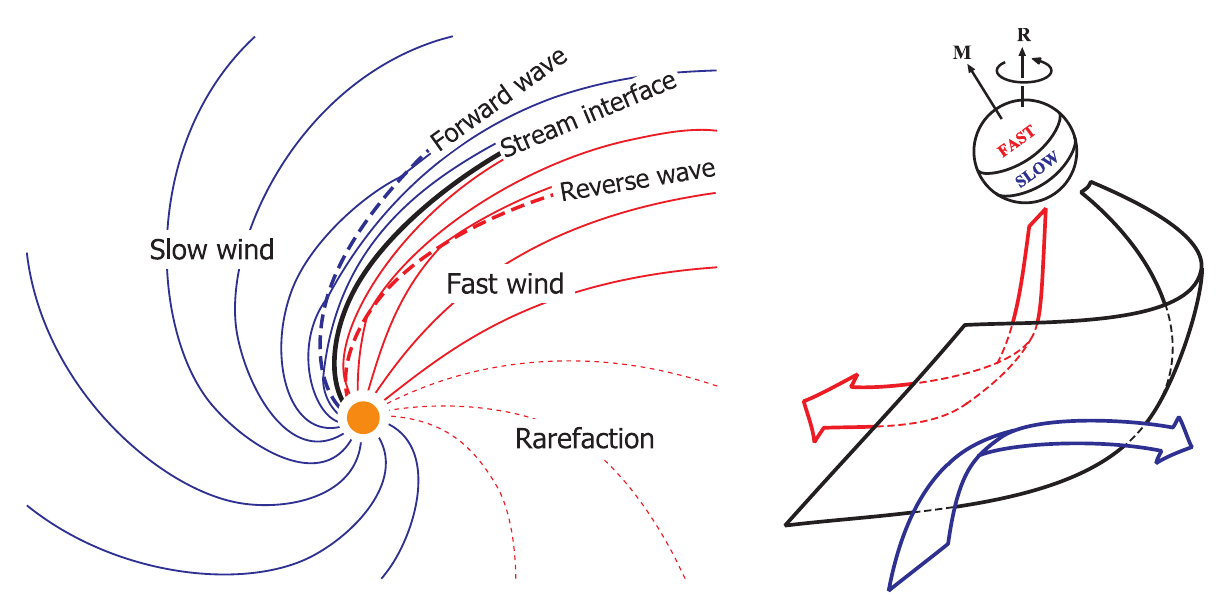
\includegraphics[width=0.6\textwidth]{figures_of_others/images/Owens2013_CIR_2panel_screenshot.png}
	}{
		\caption[\lofimage{figures_of_others/images/Owens2013_CIR_2panel_screenshot.png}Credit: {\citet[Fig.~7]{Owens2013}}; right panel adapted from {\citet[Fig.~2]{Pizzo1991}}, licensed under \href{https://creativecommons.org/licenses/by-nc/3.0/de/}{CC BY-NC 3.0 DE}.]
		{Schemata of the formation of a stream interface (left) and the deflection of streams along the interface (right). The stream interface (black) is located between regions of slow (blue) and fast (red) solar wind. Credit: {\citet[Fig.~7]{Owens2013}}, right panel adapted from {\citet[Fig.~2]{Pizzo1991}}, licensed under \href{https://creativecommons.org/licenses/by-nc/3.0/de/}{CC BY-NC 3.0 DE}.}
		\label{fig:Owens2013_CIR_2panel_screenshot}
	}
\end{figure}
%Owens2013 figure permission request: open access article
%A sketch of a stream interaction region. Left: Looking down on the ecliptic plane. Magnetic field lines within fast (slow) wind, shown in red (blue), become aligned with the stream interface by the reverse (forward) wave. Right: a view from Earth. The magnetic axis, M, and therefore the wind speed belts, are inclined to the rotation axis, R. The point in the heliosphere at which fast wind is able to catch up to the slow wind ahead of it is the stream interface (SI), which forms a spiral front in the heliosphere, shown as the black-outlined curved surface. In the frame of reference of the SI, both fast and slow wind flow toward the SI. Fast (slow) wind, shown by the red (blue) arrow, is slowed (accelerated) and deflected along the SI in the direction counter to (along) solar rotation. Right panel adapted from Pizzo (1991).

% CIRs
When the solar dipole field is in a quasi-stable configuration, SIRs can stay for multiple solar rotations, recurrently sweeping over the heliosphere in 27-day periods \citep{Gosling1972}. Hence, they are referred to as co-rotating interaction regions (CIRs) \citep{Smith1976,Balogh1999}.
% time
In the ecliptic at \SI{1}{\au}, CIRs occur commonly during the declining phase of the solar cycle when polar CHs form equatorial extensions \citep{Balogh2009}.

% deflections
The spiral shape of the stream interfaces and their inclination to the solar rotation axis lead to a deflection of both streams \citep{Balogh2009}. Due to the fast and slow streams' collision, the fast wind is decelerated whereas the slow wind is accelerated. Their flow directions are systematically deflected away from the interface, as shown in the right panel of \autoref{fig:Owens2013_CIR_2panel_screenshot}.

% shocks
The plasma pressure inside SIRs is increasing with heliocentric distance and therefore, the leading and trailing compressional waves form into foreward and reverse shocks -- typically at solar distances between \SIrange{2}{10}{\au} \citep{Smith1976,Balogh2009}. The solar wind speed increases abruptly at both shock fronts.
% MIRs
With increasing solar distance, the leading and trailing shock fronts travel away from the stream interface. This widens the interaction regions and eventually they catch up on the close-by interaction regions \citep{Burlaga1984}. Beyond \SI{10}{\au} they fuse to merged interaction regions, which are narrower and more compressed \citep{Burlaga1985}.

% in-situ signatures of SIRs
Due to the compression within SIRs, the magnetic field strength and the plasma density are higher than in the ambient streams. These signatures can be seen in the in-situ solar wind plot in \autoref{fig:ACE_64s_v7_thesis_CIRs_2013-5-1_65_plot}. The CIRs on 5~May, 1~June, and 29~June 2013 are followed by recurrent HSSs and they contain sector boundaries as well. They are not yet accompanied by strong shocks owing to the measurement location at \SI{1}{\au}.


\subsection{Heliospheric current sheet}
The heliospheric current sheet (HCS) is the boundary surface between solar wind streams of opposite magnetic polarity. It is formed by open magnetic fluxes, expanding from both sides over closed field regions and coming into contact above. At the boundary between open and closed fields, local coronal plasma gets released and flows slowly between the fast wind streams along the current sheet into the heliosphere, creating a helmet streamer. This is why near the Sun, the HCS is typically located within slow solar wind stemming from the coronal streamer belt \citep{Owens2013}. However, with increasing solar distance, the shock wave of an adjacent SIR can pass the HCS, so that sector boundaries are often found to be embedded within SIRs \citep{Gosling1999}.

% heliospheric plasma sheet
When sector boundaries in the solar wind are observed in~situ, they show significant depletions in $\text{He}^{++}\!/\text{H}^+$ values \citep{Borrini1981}. The other solar wind parameters, such as velocity, density, and temperature, change with distance from the HCS as well \citep{Smith2001}. The HCS region itself is quite narrow with a thickness of around \SIrange{3000}{10000}{\km}; it is embedded in a region of 20--30~times its thickness, the heliospheric plasma sheet (HPS) \citep{Winterhalter1994}. The HPS contains the magnetic polarity reversal and is of low magnetic field strength and high density, resulting in a significantly enhanced value of plasma beta \citep{Crooker2004}. In the slow solar wind, the HPS can also be identified from its particularly low specific entropy, arising from its low temperature and high density \citep{Kilpua2016}.


\subsection{Coronal mass ejections}
\label{sec:coronal_mass_ejections}
Coronal mass ejections (CMEs) are eruptions of coronal magnetized plasma, which expand within hours to bubbles with sizes of several solar radii. They continuously expand further while moving farther away from the Sun into the heliosphere with velocities often surpassing even the high speed solar wind. When measured in-situ in interplanetary space, they are often called interplanetary CMEs (ICMEs). Such transient structures are found to be shot into the ambient slow and fast solar wind streams. ICMEs typically have durations of a few days. They make up about \SI{5}{\percent} of the solar wind's flow share during solar cycle minima, but can represent up to about \SI{50}{\percent} during solar cycle maxima \citep{Richardson2012}. Indeed, their frequency correlates with the sunspot number \citep{Hildner1976} and follows solar activity in amplitude and phase \citep{Webb1991}.

Long before the origins of geomagnetic disturbances were actually attributed to CMEs, a solar influence was identified as their source by \citet{Carrington1859}. However, CMEs turned out to be the major drivers for strong geomagnetic storms, because they carry the most extreme conditions found in the solar wind. Thus, they are of major importance to space weather -- their impacts on the terrestrial magnetosphere are covered in \autoref{sec:space_weather}.

% CME formation, flares
Here I cover the CME formation processes only briefly, because this work is focused on in-situ measurements. Generally speaking, CMEs are products of the instability in the coronal magnetic field. The solar differential rotation wraps the coronal magnetic field, which is rooted at the surface. Accumulated tension and emerging magnetic flux eventually initiate sudden field reconfigurations. These field line reconnections result in a lower state of potential energy, releasing a lot of energy in form of solar X"~ray flares and CMEs. Indeed, CMEs are often associated with flares and eruptive prominences, coming from their source regions \citep{Webb1987}. The sources of CMEs are located near bipolar regions and are frequently identified with eruptive prominences \citep{Subramanian2001}.

% flux ropes, filaments, prominences
CMEs emerge from coronal magnetic flux rope structures that hold plasma filaments embedded along their base \citep{Webb1987,Cremades2004}. Reconfiguration of the ambient magnetic field can lead to a release and a subsequent ascend of the flux rope through the corona. During this process, the filament is lifted by the flux rope and forms a prominence eruption. The accompanying sudden magnetic reconnections often cause a multitude of other dynamic coronal phenomena: enhanced X"~ray flaring; the formation of post-eruptive arcades where the filament disappeared; local decreases in soft X"~ray intensity (coronal dimmings) due to depletion of the plasma density caused by magnetic field expansion; and large-scale coronal disturbances observed in extreme ultraviolet (EUV"~waves) that can spread across the whole corona.

% SEPs and radio bursts
The onset of CMEs is often accompanied by solar energetic particles (SEPs) and by solar radio bursts. SEPs consist of protons, electrons, and ions with relativistic energies that can cover the distance to Earth within half an hour and pose a radiative threat to humans in space. The intensity of energetic protons correlates well with the CME speed \citep{Kahler1978} and it is established that these coronal particles are accelerated by shocks formed in front of the rapidly expanding magnetic structures of CMEs in the corona \citep{Cliver1982,Gosling1993}. Solar radio bursts are radio emissions from the corona that change over time in frequency space. There are different kind of radio bursts, but especially type~II radio bursts are seen as indicators for coronal shocks that accelerate electrons. 
They are emitted in the low corona and are drifting to lower frequencies over time. There is still a debate whether type~II bursts originate from flares or CMEs, favoring the latter \citep{Gosling1993,Cliver2005,Cho2011}.
% % radio bursts
% % https://www.nrao.edu/astrores/gbsrbs/Pubs/AJP_07.pdf
% % http://www.astron.nl/lofarscience2015/Documents/LSW/June_2/Session_3/reid.pdf
% A solar radio burst is a structure in frequency space that changes with time.\\
% type~II radio burst (drift to low frequencies): fundamental and second–harmonic bands; evidence for shocks in the corona, rendered visible by the radiation of electrons that they accelerate. There is almost always a delay between the flare onset and the start of Type II emission. the shocks that produce Type II bursts are maybe always being driven by CMEs\\
% type~III radio burst (spikes): parallel to flares; track electron beams through decreasing sw plasma density along Parker spiral; frequency scales with distance\\
% type~IV radio burst: broadband quasi–continuum features associated with the decay phase of solar flares. They are attributed to electrons trapped in closed field lines in the post–flare arcades\\

CMEs were detected in the white-light observations of the K"~corona made by the first space-based coronagraphs on board the OSO~7 satellite \citep{Tousey1973} and the Skylab space station \citep{MacQueen1974}. These observations show the steady outflow of solar wind, broken by intermittent ejections of coronal plasma. Subsequently, the kinematic properties of CMEs were identified from the white-light images \citep{MacQueen1980}. Now, coronagraphs observe the corona and hence CMEs continuously from the first Lagrange point (L1) in front of Earth with the SOHO spacecraft and from changing equatorial perspectives with the STEREO~Ahead (A) and Behind (B) spacecraft. The image of the corona from 26~February 2000, made by the LASCO/C3 coronagraph on board SOHO, shows such a CME with a detailed three-part structure, see \autoref{fig:20000226_lightbulb_CME_c3full}. This typical structure consists of a bright frontal loop, trailed by a dark cavity with a bright core.
\begin{figure}[htb]
	\begin{floatrow}
		\ffigbox{
			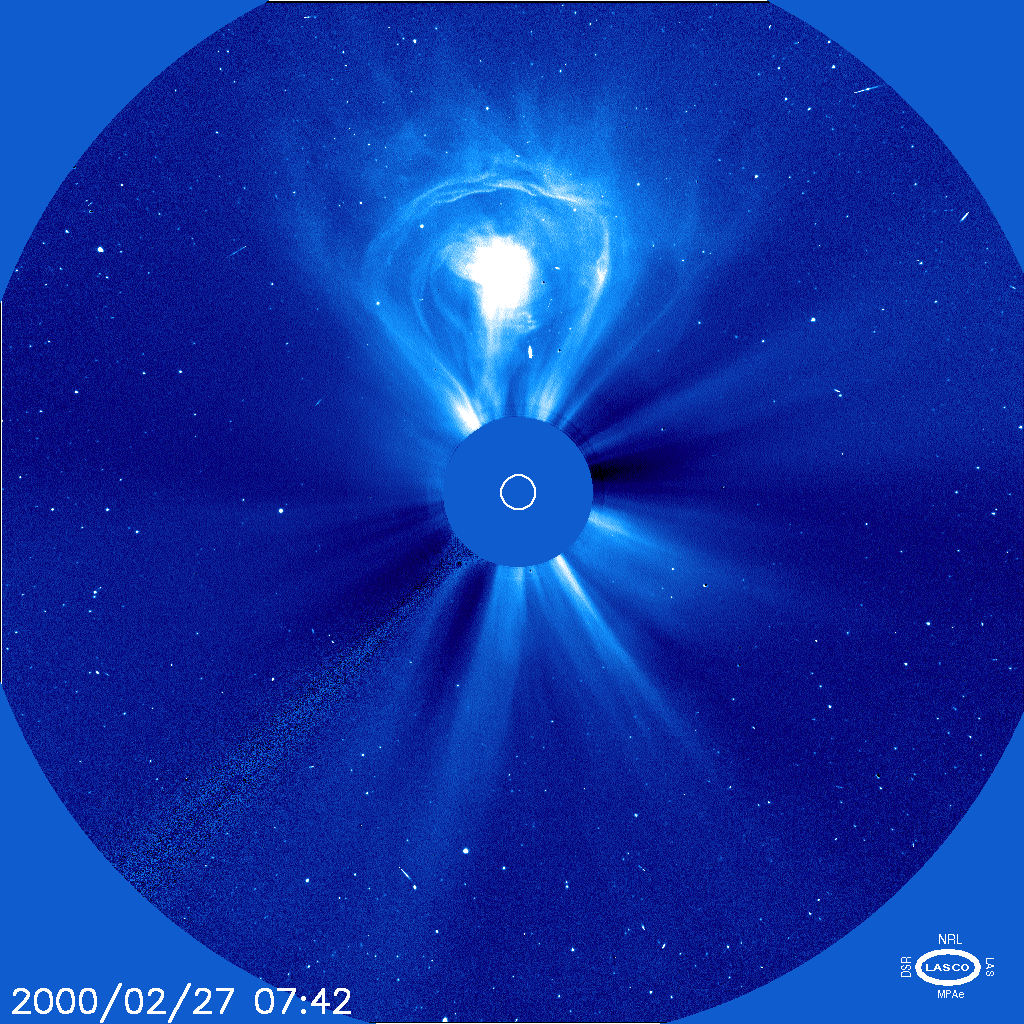
\includegraphics[width=0.46\textwidth]{figures_of_others/images/20000226_lightbulb_CME_c3full.png}
		}{
			\caption[\lofimage{figures_of_others/images/20000226_lightbulb_CME_c3full.png}Courtesy of SOHO/LASCO consortium. SOHO is a project of international cooperation between ESA and NASA.]
			{Image of the solar corona out to \SI{30}{\Rs} from 26~February 2000 taken by the LASCO/C3 coronagraph on board the SOHO spacecraft. The solar disk is covered by the occulter disk and its position is indicated by the white circle. The bright blob at the top is a CME with a detailed three-part structure; the smooth elongated radial lines are solar wind streamers. Courtesy of SOHO/LASCO consortium; SOHO is a project of international cooperation between ESA and NASA.}
			\label{fig:20000226_lightbulb_CME_c3full}
		}
% https://sohowww.nascom.nasa.gov/hotshots/2000_02_26/
% https://sohowww.nascom.nasa.gov/data/summary/copyright.html
		\ffigbox{
			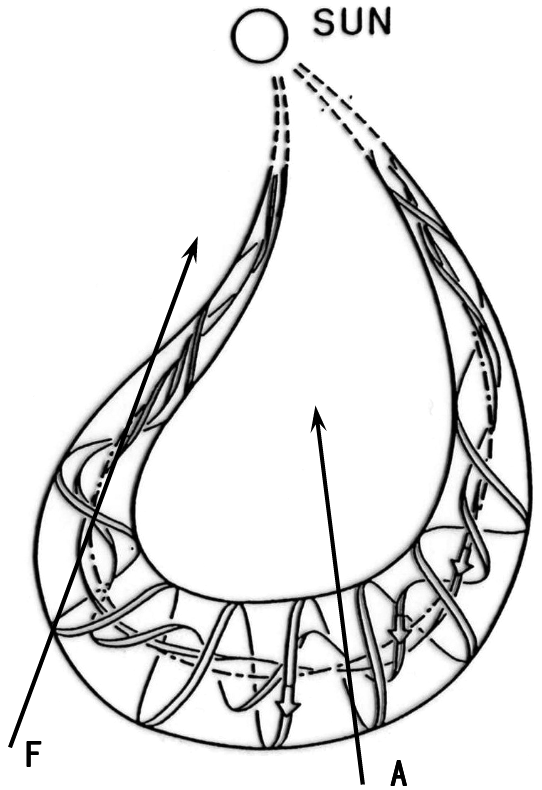
\includegraphics[width=0.31\textwidth]{figures_of_others/images/Marubashi2007_fig1.png}
		}{
			\caption[\lofimage{figures_of_others/images/Marubashi2007_fig1.png}Credit: {\citet[Fig.~1, panel (a)]{Marubashi2007}}, licensed under \href{https://creativecommons.org/licenses/by/3.0/}{CC BY 3.0}.]
			{Schema of a magnetic flux rope structure in a CME. The arrows depict passings through its flank (F) and its apex (A). Credit: {\citet[Fig.~1, panel (a)]{Marubashi2007}}, licensed under \href{https://creativecommons.org/licenses/by/3.0/}{CC BY 3.0}.}
			\label{fig:Marubashi2007_fig1}
		}
	\end{floatrow}
\end{figure}

It was early determined by \citet{Gold1962} that solar ejecta should drive shock waves ahead. In fact, shocks with trailing low proton temperatures caused by fast CMEs were then found in in-situ measurements \citep{Gosling1973,Gosling1974}. \citet{Burlaga1981} analyzed magnetic field and plasma data from five spacecraft and identified a shock wave with a trailing turbulent sheath region followed by an organized helical magnetic structure that they called a magnetic cloud (MC). MCs have an enhanced magnetic field, a smooth rotation in the magnetic field vector and they show low densities and temperatures \citep{Burlaga1981}. Thus, MCs have a low thermal to magnetic pressure ratio (i.e., a small plasma beta) and the magnetic field dominates the plasma. Furthermore, the overall pressure in MCs is higher than in the ambient solar wind, resulting in the expansion of MCs on their way out. Shock-driving CMEs containing a helical MC are actually identified with magnetic flux ropes that expand self-similarly and that remain in connection with the solar surface \citep{Chen1997}. The surface connection is indicated by bi-directional streams of electrons that are found in MCs \citep{Gosling1986}. The shape and magnetic topology of such a magnetic flux rope is pictured in \autoref{fig:Marubashi2007_fig1}. It is apparent that in-situ measurements should look significantly different depending on where the CME is pierced.

% BSS
Such solar wind in-situ measurements reveal the magnetic structure of CMEs. In  particular, the orientation of magnetic flux ropes can be determined by applying a minimum variance analysis (MVA) to the MCs' magnetic field components \citep{Sonnerup1967,Burlaga1982}. An MVA determines the direction of minimum variance in the sequence of field vectors passing by during an MC encounter. The principal axis of the flux rope can be derived from the pattern of the field components orthogonal to the direction of minimum variance.

\citet{Bothmer1998} used the MVA on an extensive set of MCs which they found in the data of the Helios~1 and~2 probes. They related the results with the magnetic polarity structures of the MCs' apparent solar source regions. Connecting the derived flux rope directions with the orientation of disappearing filaments and magnetic neutral lines on the solar surface, they recognized a scheme that is able to infer the orientation and helicity of MCs found in CMEs. This Bothmer-Schwenn scheme (BSS) relates these magnetic flux rope properties to whether the solar cycle number is even or odd and depending on which solar hemisphere the CME originates from (northern/southern) -- utilizing that the hemispheric polarity is alternating with each solar cycle, see \autoref{fig:Bothmer1998_fig18}. As the probability is greater than \SI{80}{\percent} that the magnetic topology of an active region conforms to the hemispheric rule \citep{Wang2013}, an MC configuration predicted with the BSS is expected to have a reliability that is of the same order \citep{Savani2015}.
\begin{figure}[p]
	\centering
	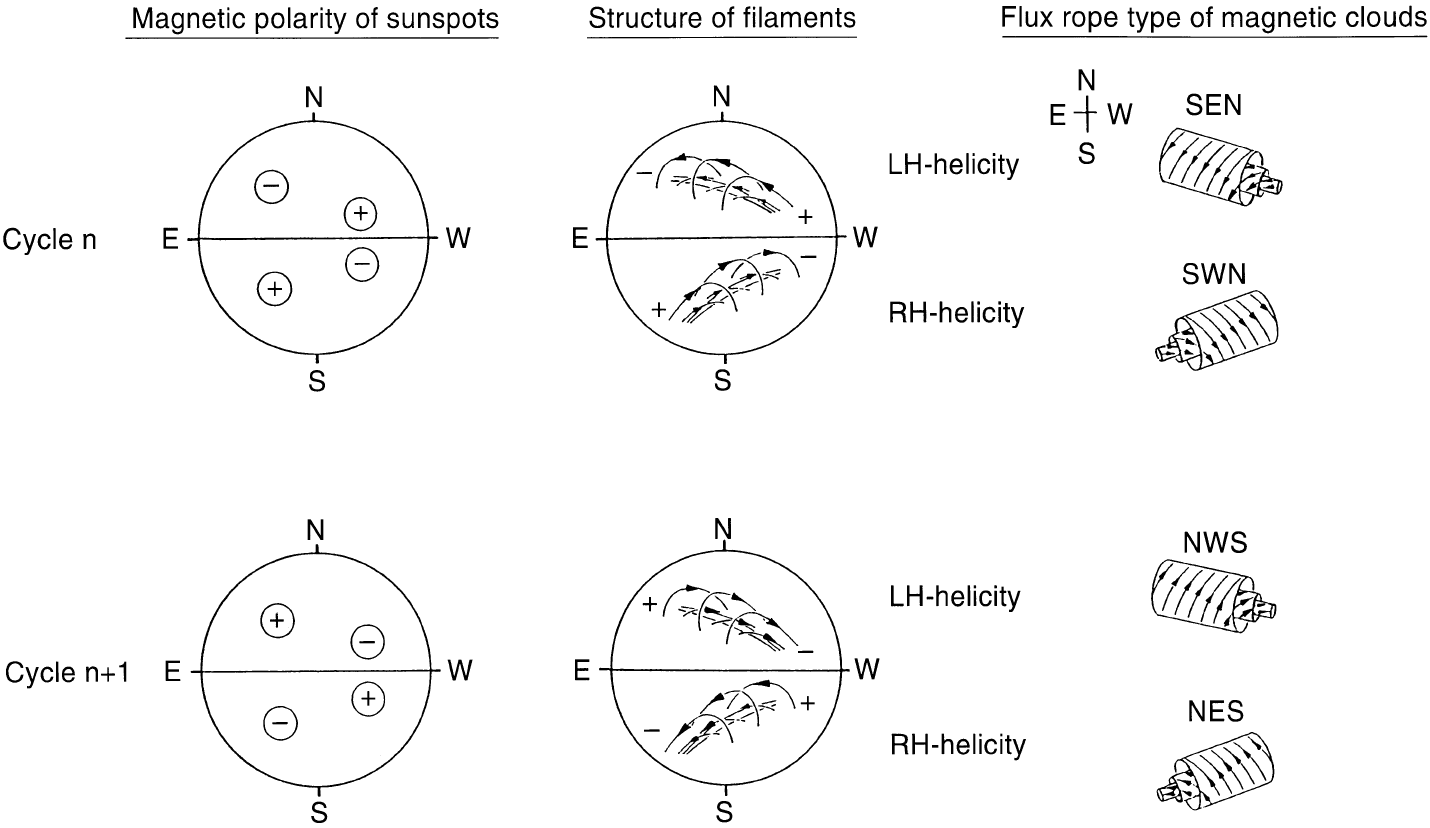
\includegraphics[width=\textwidth]{figures_of_others/images/Bothmer1998_fig18.png}
	\caption[\lofimage{figures_of_others/images/Bothmer1998_fig18.png}Credit: {\citet[Fig.~18]{Bothmer1998}}, \textcopyright~EGS -- Springer-Verlag, reproduced with permission.]
	{Explaining sketch of the BSS. The two rows represent odd ($n$) and even ($n + 1$) solar cycle numbers. The magnetic polarity of sunspots, the structure of filaments, their helicity, and the corresponding flux rope type of magnetic clouds are shown. Credit: {\citet[Fig.~18]{Bothmer1998}}, \textcopyright~EGS -- Springer-Verlag, reproduced with permission.}
	\label{fig:Bothmer1998_fig18}
\end{figure}

% CME in-situ plot
Three CMEs can be seen in the solar wind in-situ measurements showed previously in \autoref{fig:ACE_64s_v7_thesis_CIRs_2013-5-1_65_plot}, passing by the ACE spacecraft at L1 on 24~May, 6~June, and 27~June in 2013. The latter CME has a well-structured MC, which is presented in detail in \autoref{fig:ACE_64s_v7_thesis_CME_2013-6-26_6} -- I use this event as an example throughout this section.
\begin{figure}[p]
	\centering
	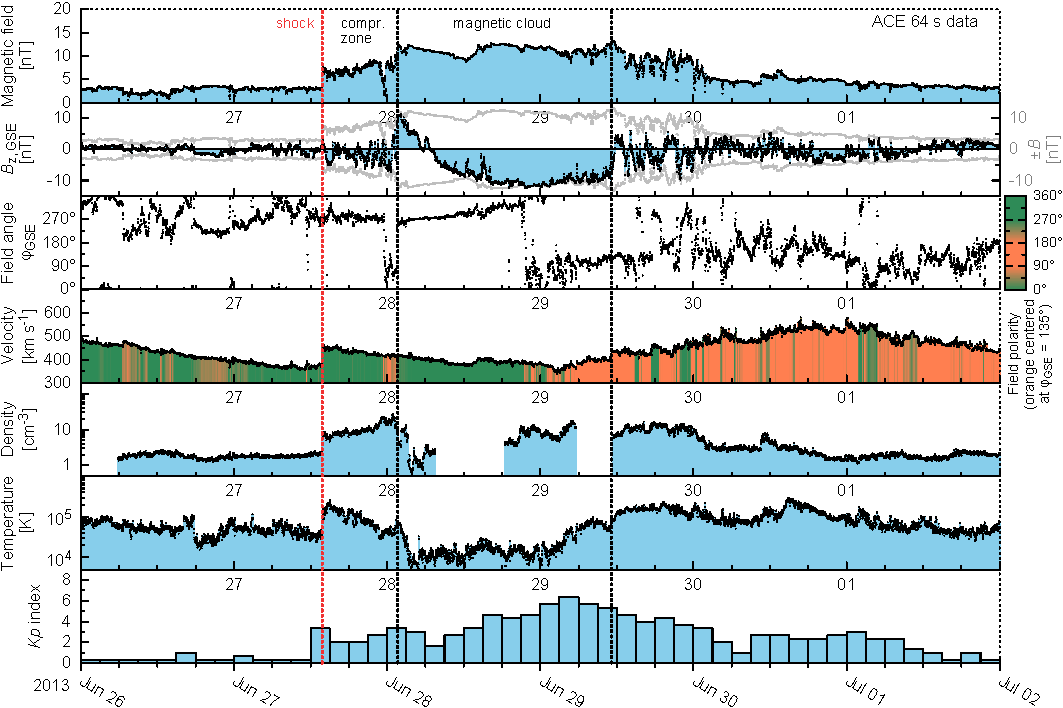
\includegraphics[width=\textwidth]{figures_of_mine/gnuplots/ACE_64s_v7_thesis_CME_2013-6-26_6.pdf}
	\caption[\lofimage{figures_of_mine/gnuplots/ACE_64s_v7_thesis_CME_2013-6-26_6.pdf}I created the figure myself.]
	{Solar wind with a CME signature, measured at L1 during the time period 26~June to 2~July in 2013. The solar wind parameters are the magnetic field strength, its z-component and ecliptic field angle in GSE~coordinates, the proton velocity, density, and temperature; in addition, the geomagnetic \Kp~index is plotted in the bottom panel. In the velocity panel also the field polarity is color coded -- assuming a fixed Parker spiral angle of \SI{135}{\degree}. I indicated the shock, the compression zone, and the duration of the magnetic cloud with dotted lines. Blank periods indicate bad or missing data. The solar wind data was measured with the MAG and SWEPAM instruments on board the ACE spacecraft and is obtained from the ACE~Science~Center. The \Kp{}~data is obtained from the GFZ~Potsdam.}
	\label{fig:ACE_64s_v7_thesis_CME_2013-6-26_6}
\end{figure}
In addition to presenting the solar wind in-situ parameters, I indicated the shock, the compression zone, and the MC with dotted lines, and added the geomagnetic \Kp{}~index in order to visualize the CME's impact on the magnetosphere. This MC contains a sector boundary and is trailed by an interaction region caused by a following HSS.

\pagebreak

The CME occurred in solar cycle~24. The MC's IMF z"~component changes from positive (northern) to negative (southern) values -- during this process, the field angle in the ecliptic, $\phi$, stays pointing roughly towards \SI{270}{\degree} (west). Thus, it has a NWS configuration, which is expected from the BSS during even numbered solar cycles for CMEs with source regions located in the northern hemisphere.

%white-light structure
The combination of white-light images with in-situ data enables relating the observed structures of CMEs. Even disturbances in front of fast CMEs can be identified as shock waves in the white-light images made by the SOHO coronagraph \citep{Sheeley2000}. The diffuse leading feature of a CME is the shock sheath, its brightness is caused by the density jump after the shock, which itself is not visible in coronagraphs. The trailing void is identical to the low density of the magnetic flux rope, which drives the whole structure.

The CME described before is indeed coming from the northern hemisphere, as can be seen from the STE\-REO~A coronagraph image displayed in \autoref{fig:STEREO_A_COR2_20130624_022400_dbc2A} taken three days earlier. Apparently, the CME reaches into the ecliptic so that its lower portion passes Earth. Also in this image, the event originates behind the solar limb, considering the observing spacecraft's position in relation to Earth at that time, see \autoref{fig:STEREO_positions_w_269707595}.
\begin{figure}[htb]
	\begin{floatrow}
		\ffigbox{
			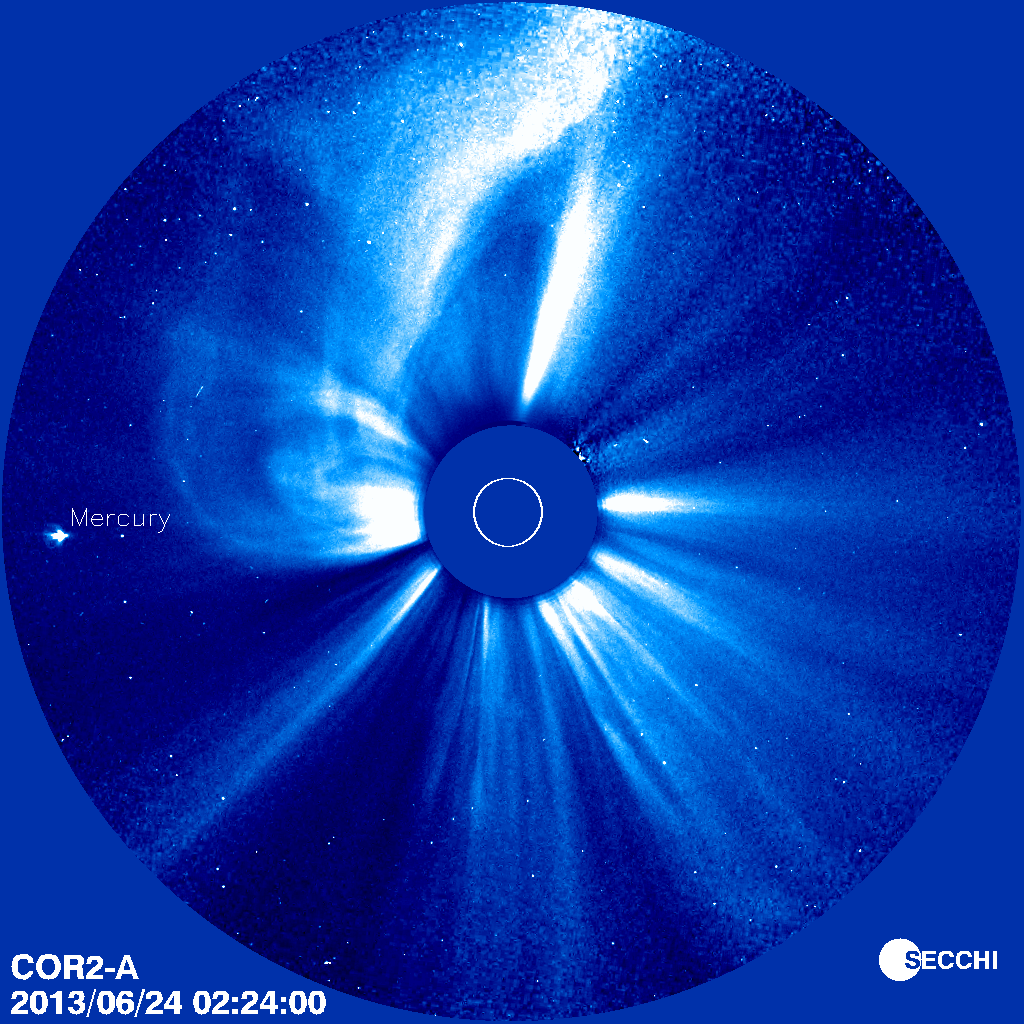
\includegraphics[width=0.46\textwidth]{figures_of_others/images/STEREO_A_COR2_20130624_022400_dbc2A.png}
		}{
			\caption[\lofimage{figures_of_others/images/STEREO_A_COR2_20130624_022400_dbc2A.png}Courtesy of \href{https://stereo.gsfc.nasa.gov/gallery/copyright.shtml}{STEREO/COR2 consortium (NASA)}.]
			{Image of the solar corona out to \SI{15}{\Rs} from 24~June 2013 taken by the SECCHI/COR2 coronagraph on board the STEREO~A spacecraft. The solar disk is covered by the occulter disk and its position is indicated by the white circle. The CME is the extended structure to the upper left; the smooth elongated radial lines are solar wind streamers. Courtesy of \href{https://stereo.gsfc.nasa.gov/gallery/copyright.shtml}{STEREO/COR2 consortium (NASA)}.}
			\label{fig:STEREO_A_COR2_20130624_022400_dbc2A}
		}
% https://secchi.nrl.navy.mil/sccimages/
% https://stereo-ssc.nascom.nasa.gov/browse/2013/06/24/index.shtml
% https://stereo.gsfc.nasa.gov/gallery/copyright.shtml
		\ffigbox{
			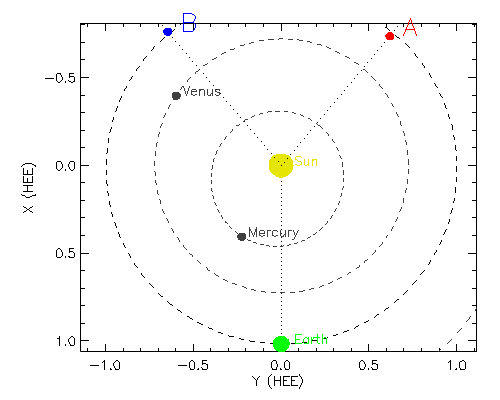
\includegraphics[width=0.46\textwidth]{figures_of_others/images/STEREO_positions_w_269707595.png}
		}{
			\caption[\lofimage{figures_of_others/images/STEREO_positions_w_269707595.png}This figure is made with the online \href{https://stereo-ssc.nascom.nasa.gov/cgi-bin/make_where_gif}{STEREO Orbit Tool} at the STEREO Science Center website.]
			{Positions of the STEREO~A and~B spacecraft relative to Sun and Earth for 24~June 2013 02:24~UT. This figure is made with the online \href{https://stereo-ssc.nascom.nasa.gov/cgi-bin/make_where_gif}{STEREO Orbit Tool} at the STEREO Science Center website\protect\footnotemark.}
			\label{fig:STEREO_positions_w_269707595}
		}
% https://stereo-ssc.nascom.nasa.gov/cgi-bin/make_where_gif
	\end{floatrow}
\end{figure}
\footnotetext{STEREO Science Center website: \urlfoot{https://stereo-ssc.nascom.nasa.gov/}}

% CBS
Relating CME white-light images to observations of magnetic neutral lines on the solar surface, \citet{Cremades2004} interpreted the white-light appearances of CMEs as projections of their 3D geometry and developed a scheme for their orientation depending on the orientation and location of the neutral lines on the solar surface. Neutral lines on the solar surface are the lines of polarity inversion between two areas of opposite magnetic polarity. The scheme is based on the topology of the flux rope model and the observation that its major axis stays roughly aligned to the underlying neutral line during the eruption process. Thus, \citet{Cremades2004} concluded that CMEs look systematically different depending on their source region's position and magnetic configuration, as described in \autoref{fig:Cremades2004_fig15}.
\begin{figure}[htb]
	\centering
	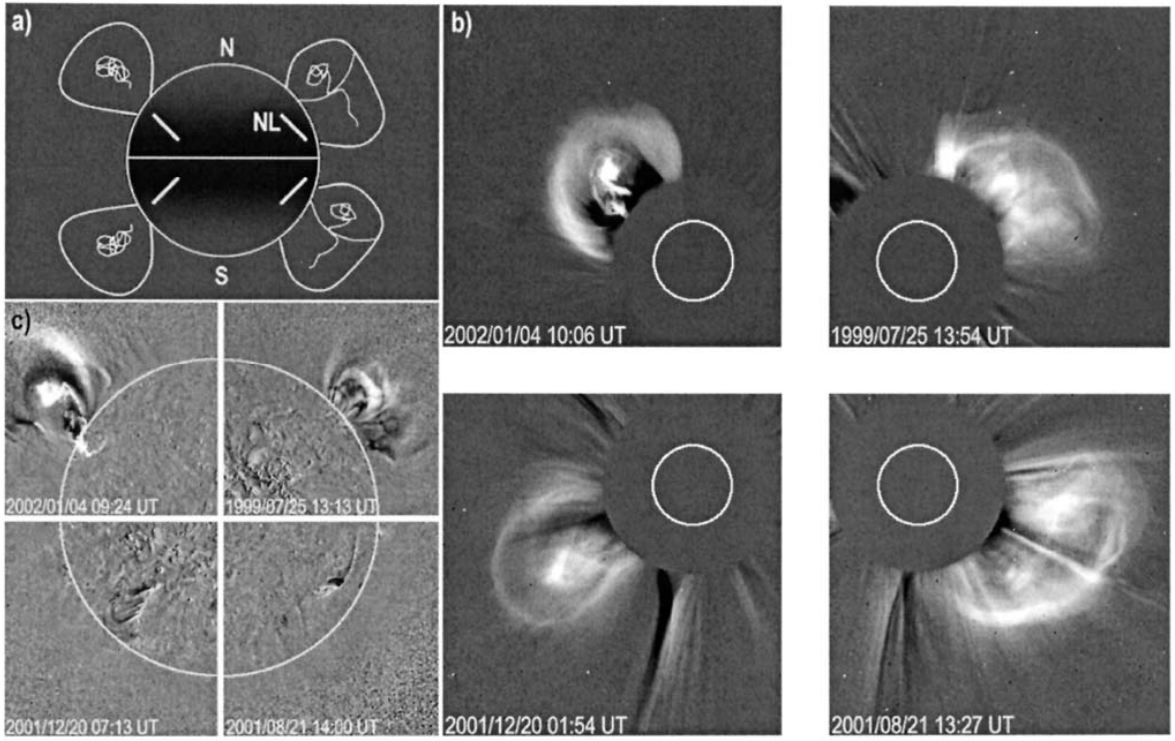
\includegraphics[width=\textwidth]{figures_of_others/images/Cremades2004_fig15.png}
	\caption[\lofimage{figures_of_others/images/Cremades2004_fig15.png}Credit: {\citet[Fig.~15]{Cremades2004}}, \textcopyright~ESO, reprinted with permission.]
	{White-light CME projection scheme for front-side events, showing the case for each quadrant of the solar disk. (a)~Schema showing the expected white-light appearance of CMEs and the orientation of the underlying magnetic neutral lines. (b)~White-light images of CME example events, made with the LASCO C2 coronagraph on the SOHO spacecraft. (c)~Details (prominences and post-eruptive arcades) of the source regions related to the CMEs shown in panel~(b). Note that for events originating from the backside, panel~(a) has to be mirrored vertically. Credit: {\citet[Fig.~15]{Cremades2004}}, \textcopyright~ESO, reprinted with permission.}
	\label{fig:Cremades2004_fig15}
\end{figure}
For the solar backside, the neutral lines are reversed and according to the scheme so are the CME orientations -- thus the broad CME appearing behind the solar limb seen in \autoref{fig:STEREO_A_COR2_20130624_022400_dbc2A} matches this scheme. The scheme can effectively be applied for CMEs with source regions located less than \SI{50}{\degree} from the solar equator \citep{Webb2012}.

This white-light CME projection scheme as well as the BSS for MCs are based on the notion that the orientation of flux ropes propagating outwards generally stays aligned with the neutral polarity inversion line on the solar surface where the filament erupted \citep{Marubashi1997,Bothmer1998}. In fact, it is shown that flux ropes are not likely to rotate significantly after their initiation but commonly maintain the orientation of their main axis parallel to the magnetic neutral line\pagebreak even in interplanetary space \citep{Marubashi2015}. However, during and shortly after their eruption, CMEs are frequently observed to be deflected to other directions by the surrounding coronal magnetic field structure \citep{Sterling2011}.

% CME redefinition
The revelation that all CMEs may be flux ropes \citep{Vourlidas2013,Marubashi2015} led to the expansion of the CME definition based on white-light images made by \citet{Hundhausen1984}. \citet{Vourlidas2013,Vourlidas2014} include magnetic flux ropes in their recent CME redefinition: \textit{``A CME is the eruption of a coherent magnetic, twist-carrying coronal structure with angular width of at least \SI{40}{\degree} and able to reach beyond \SI{10}{\Rs} which occurs on a time scale of a few minutes to several hours.''}

% flux rope distortion
However, CMEs generally do not have a perfect flux rope geometry: Often their more complex structure can be seen in kinks of the corresponding filament before the eruption \citep{Bothmer2017}; and strong distortions can happen during the eruption process. Their cross section is only initially of circular shape, it distorts due to the pressure-driven self-expansion and the radial solar wind expansion \citep{Owens2006}. Though, the inner core of the flux rope is believed to stay of circular shape. For these reasons, the properties of CMEs vary widely and imaging projection effects contribute further to that \citep{Cremades2004}.

%open questions
There still exist a lot of unresolved questions about CMEs, their formation, and the effects observed along with them: Multiple mechanisms/processes are debated for the release of CMEs and their subsequent acceleration. It is also not known if there exist CMEs without magnetic flux ropes \citep{Vourlidas2013}. The relation between flux ropes observed in the near-Sun corona and measured in~situ at interplanetary distances is still not entirely clear \citep{Vourlidas2014}. Nobody knows yet when a CME will erupt on the Sun, at what exact time it will pass a given point in the heliosphere, and how its detailed magnetic configuration would look like in~situ \citep{Gopalswamy2016}.

%white-light images of a backside CME\\
% SOHO LASCO CME CATALOG
% 2013/06/24 	04:00:05 	Halo 	
% https://cdaw.gsfc.nasa.gov/CME_list/UNIVERSAL/2013_06/univ2013_06.html
% https://cdaw.gsfc.nasa.gov/movie/make_javamovie.php?stime=20130624_0236&etime=20130624_0714&img1=lasc2rdf&title=20130624.040005.p235g;V=709km/s

% Sun Earth Connection Coronal and Heliospheric Investigation (SECCHI) on board the Solar Terrestrial Relations Observatory (STEREO) spacecrafts \citep{Howard2008}\\

% literature:
% historical CME review by \citet{Gopalswamy2016}.\\
% historic review; Syun-Ichi Akasofu2011\\


%%%%%%%%%%%%%%%%%%%%%%%%%%%%%%%%%%%%%%%%%%%%%%%%%%%%%%%%%%

% Space weather
%
% Magnetosphere
% Structure (currents, plasma regions)
% Solar wind coupling mechanisms (list all: reconnection, turbulence, ...)
% Dungey convection cycle (unsteady/continuous reconnection; substorms; two-cell convection)
% Russell-McPherron effect (seasonal variations)
% Geomagnetic indices
%
% Geomagnetic storms (difference to substorms; types of triggering events (CMEs, CIRs, Dst, ...)
% Kp index
%
% Geomagnetic activity forecast
% Coupling functions
% Kp forecast methods (empirical functions, neural networks, model list)
% CME and stream forecast to Earth (incl. storm causes; methods and model list)

%%%%%%%%%%%%%%%%%%%%%%%%%%%%%%%%%%%%%%%%%%%%%%%%%%%%%%%%%%

\clearpage

\section{Space weather}
\label{sec:space_weather}
Space weather is the field of research that comprises all dynamic effects generated by the Sun itself but also from cosmic rays in
the Sun's domain of influence -- the heliosphere. Naturally, space weather is especially focused on the solar effects observed on Earth and in its local environment -- the ionosphere and the magnetosphere. There exist several different effects caused by independent solar events occurring on different time scales that can affect humans directly or indirectly. Solar events affect sensitive technical systems and strong events are even able to disrupt them and pose a threat to humans \citep{Bothmer2007}. Space weather deals with effects on time scales similar to the terrestrial weather, that is, hours, days, and weeks.

The existence of a direct solar-terrestrial relation was known of early on. \citet{Carrington1859} made the first connection between solar flares and disturbances in the terrestrial magnetic field when he observed a brightening on the solar disk on 1~September 1859 and suggested its connection to a strong geomagnetic storm that occurred about 17~hours later. Categories of solar-terrestrial correlations were already listed by \citet{Bartels1962}: Events initiated by irregular solar X"~ray flares and CMEs, by the 11"~year solar activity cycle, and by the periodic 27"~day solar rotation. Other time related variations include seasonal effects caused by the Earth's orbital distance oscillation over the year and the inclinations of the Sun's and Earth's rotation axes to the ecliptic normal. The terrestrial magnetic field's dipole axis tilt to the rotation axis further contributes to the daily effects.

The major driving forces behind severe space weather events are CMEs, solar X"~ray flares, and solar energetic particle (SEP) events. Most of the terrestrial space weather effects are introduced through the events' influence on the magnetosphere, ionosphere, and upper atmosphere. Space weather effects, commonly classified into geomagnetic storms, solar radiation storms, and radio blackouts\footnote{NOAA Space Weather Scales website: \urlfoot{https://www.swpc.noaa.gov/noaa-scales-explanation}}, are listed in the following.

The solar wind's internal structures, such as CMEs and CIRs, affect the magnetosphere and can cause large disturbances in its magnetic field. These disturbances are called geomagnetic storms and are described in more detail in \autoref{sec:geomagnetic_storms}. Notable consequences of these major disturbances in the terrestrial magnetic field are listed below \citep{Bothmer2007}:
\begin{itemize*}
	\item The auroral oval shifts to lower latitudes and the auroral activity is enhanced\footnote{NOAA/SWPC Tips on Viewing the Aurora: \urlfoot{https://www.swpc.noaa.gov/content/tips-viewing-aurora}}.
	\item The equatorward auroral oval shift leads to direct risks for humans from enhanced radiation doses during high altitude flights through an enlarged polar cap\footnote{NOAA/SWPC Galactic Cosmic Rays: \urlfoot{https://www.swpc.noaa.gov/phenomena/galactic-cosmic-rays}}.
	\item Enhanced particle radiation in the Van~Allen belt can lead to faulting electronics and disturb satellite operations.
	\item Geomagnetic storms can rapidly heat the upper atmosphere, causing it to expand, and generate an increased drag for satellites in low Earth orbits\footnote{NOAA/SWPC Satellite Drag: \urlfoot{https://www.swpc.noaa.gov/impacts/satellite-drag}}.
	\item Geomagnetically induced currents are created in long conducting infrastructure, such as oil pipelines, rail tracks, and power lines. The currents can lead to increased steel corrosion and power grid outages.
	\item The sunward magnetopause distance can shrink under extreme solar wind pressure below the geostationary Earth orbit (GEO) at a distance of \SI{6.6}{\RE}. GEO satellites crossing the magnetopause are then directly exposed to the radiation of SEPs.
	\item The magnetic navigation and behavior of animals, such as migratory birds \citep{Moore1977} and whales, is influenced \citep{Vanselow2017}.
\end{itemize*}

Solar extreme ultraviolet (EUV) and X"~ray radiation events (solar flares) affect the ionosphere apart from the radiation's regular day/night cycle influence. Solar flares can create sudden ionospheric disturbances \citep{Gosling1993}, that is, abrupt enhancements in the ionospheric total electron content (TEC). These TEC variations threaten the following technical systems \citep{Kraaikamp2015}:
\begin{itemize*}
	\item Increased TEC leads to larger positioning errors in global navigation satellite systems (GNSS).
	\item Scintillation and absorption of high frequency signals on their way through the ionosphere can lead to signal disturbances and loss of satellite communications.
	\item Induced changes in the stratification of the ionosphere (D-, E-, and F"~layers) disturb radio communication and lead to outages in multiple frequency bands.
\end{itemize*}

\pagebreak

Flares and CME shock fronts accelerate coronal particles, producing SEPs. These are guided by the IMF along the Parker spiral through the heliosphere. High fluxes of SEPs induce solar radiation storms with durations ranging from hours to days that have the following effects \citep{Bothmer2007}:
\begin{itemize*}
	\item Electronic circuits in satellites and spacecraft receive enhanced radiation damage.
	\item The enhanced radiation damages biological tissue in humans and organisms brought to space.
	\item SEPs are guided by the terrestrial magnetic field down to the polar regions. Thus, humans flying in aircraft near polar latitudes are exposed to higher radiation doses during strong radiation storms. Especially humans in orbit outside the protective atmosphere are endangered.
	\item Free electrons, created by SEPs colliding with the atmosphere, form ionospheric layers that disturb/block high frequency radio communications\footnote{NOAA/SWPC Solar Radiation Storm: \urlfoot{https://www.swpc.noaa.gov/phenomena/solar-radiation-storm}}.
\end{itemize*}

Obviously there also exist lots of space weather effects on the rest of the solar system bodies. Notable effects are \citep{Bothmer2007}:
\begin{itemize*}
	\item Other planetary magnetospheres are impacted in similar ways as the terrestrial is (e.g., the Jovian and Saturnian magnetospheres).
	\item Induced magnetospheres on nonmagnetic bodies, as is the case at Venus, are affected by the varying external plasma of the solar wind \citep{Luhmann2004}.
	\item The solar system regions outside of protective magnetospheres suffer directly from episodes of enhanced solar radiation, that is, from flare and SEP events.
	\item Solar wind structures can strip off cometary tails and can enhance atmospheric losses in bodies without magnetosphere.
	\item The average solar wind pressure and HMF scale with solar activity and therefore modulate the shape and size of the heliosphere. As cosmic rays are influenced by the HMF, the local cosmic ray radiation level scales inversely with solar activity. Even the passings of strong shocks and MCs lead to reductions in local cosmic ray radiation, which are called Forbush decreases.
\end{itemize*}

Most terrestrial space weather effects are connected with economic interests and some impacts on technical systems can even influence human lives. This creates strong interest in forecasting the space weather conditions of the upcoming hours and days. Space weather forecasting is a relatively new field of study, however, it becomes more and more important, not only because of the increasing use of sensitive technology at Earth, but also because of the anticipated expansion of interplanetary space activities within the near future, such as human space missions to Moon and Mars. There exist a number of dedicated institutions and forecasting techniques for the different aspects of space weather and more services are under development. This study contributes to that as one of its main foci is the forecast of the intensity of geomagnetic disturbances.

Predictions of magnetospheric disturbances are based on knowledge of the solar wind properties which the magnetosphere will encounter. Thus in a first step, forecast methods have to predict the solar wind at Earth in advance and derive its expected impact on the magnetosphere in a second step. The first part of the present study contributes to the second step with predicting the amplitude of magnetospheric disturbances caused by solar wind. The basic structure of the magnetosphere, its coupling to the solar wind, its convection cycle, and geomagnetic indices are detailed in the following \autoref{sec:magnetosphere}. \autoref{sec:geomagnetic_storms} portrays geomagnetic storms and the \Kp~index as a measure for their severity. \autoref{sec:geomagnetic_activity_forecast} describes the common solar wind coupling functions and existing methods to forecast geomagnetic disturbances and their solar wind sources.


\section{Magnetosphere}
\label{sec:magnetosphere}
In first-order approximation, the terrestrial magnetic field can be seen as a dipole aligned with the rotation axis of the Earth. Its magnetic south pole is located near the geographic North Pole and there is currently only a small tilt of about \SI{9.5}{\degree} between both axes \citep{Thebault2015} -- this angle varies slightly over the years. The magnetic field strength on the surface at the poles is around \SI{60}{\micro\tesla}, whereas at the equator it is about half that magnitude. At the Earth's surface, there are major field irregularities that deviate from the dipole approximation, such as the prominent South Atlantic Anomaly whose field is lower than \SI{24}{\micro\tesla} \citep{Thebault2015}.

The geomagnetic field's strength decreases with distance while it extends out into space. Its influence ends where its magnetic pressure balances the ram pressure of the solar wind. \citet{Gold1959} named the region governed by the terrestrial magnetic field the magnetosphere. The outer boundary is the magnetopause -- in average it has a sunward distance of about \SI{11.0}{\RE} \citep{Fairfield1971}. In response to the continuous changes in the solar wind pressure, the magnetopause usually is in a state of fast radial inward-outward motion and its displacement can reach several Earth radii \citep{DeKeyser2005}. The solar wind flow shapes the magnetopause into a surface of teardrop form, whose length of its so-called magnetotail varies around \SI{100}{\RE} and points away from the Sun.

The compression of the solar wind plasma at the front of the magnetopause creates a bow shock, whose average standoff distance to Earth is about \SI{15.1}{\RE} but varies largely under extreme solar wind conditions \citep{Fairfield1971}. The shocked solar wind plasma flows within the magnetosheath around the magnetosphere as is shown in \autoref{fig:Davies1990_magnetosphere_sharpened}.
\begin{figure}[t!]
	\fcapside[\FBwidth]{
		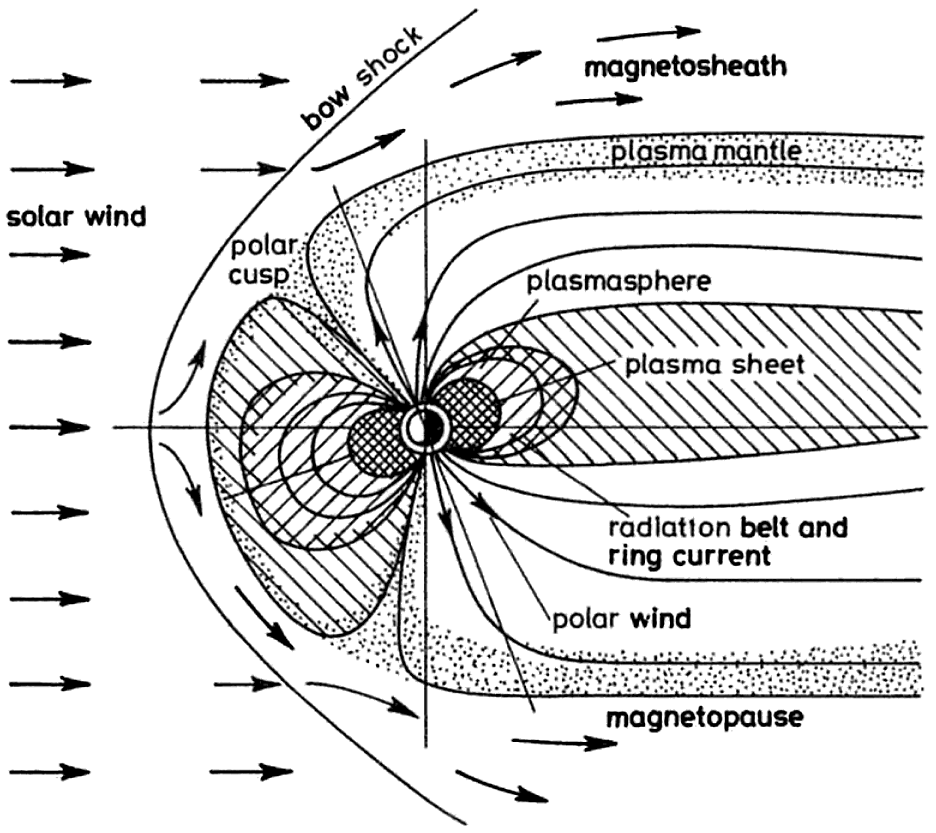
\includegraphics[width=0.6\textwidth]{figures_of_others/images/Davies1990_magnetosphere_sharpened.png}
	}{
		\caption[\lofimage{figures_of_others/images/Davies1990_magnetosphere_sharpened.png}Credit: {\citet[Fig.~2.12]{Davies1990}}, \textcopyright~IET, reproduced with permission.]
		{Schema of the magnetosphere's geometry in the plane spanned by the solar wind flow direction and the ecliptic normal (vertical line). The arrows show the flow of solar wind around the Earth's magnetic field. The diagonal line indicates the inclination of the rotation axis to the ecliptic. Credit: {\citet[Fig.~2.12]{Davies1990}}, \textcopyright~IET, reproduced with permission.}
		\label{fig:Davies1990_magnetosphere_sharpened}
	}
\end{figure}
% http://digital-library.theiet.org/content/books/ew/pbew031e
The IMF in the magnetosheath is weaker but has a larger variability than the terrestrial magnetic field on the other side of the magnetopause \citep{DeKeyser2005}.

At the front of the magnetopause, the incoming solar wind ions and electrons are being deflected in direction of dawn and dusk by the magnetospheric field, creating a current layer at the surface of the magnetopause. This current induces another magnetic field that cancels the geomagnetic field outside of the magnetopause and enhances it inside to about twice the strength of a pure dipole field at that distance \citep{DeKeyser2005}. At the magnetotail side, the magnetopause current flows into the opposite direction -- an overview, also of the inner magnetosphere's current systems is illustrated in \autoref{fig:DeKeyser2005_magnetosphere}.
\begin{figure}[htb]
	\fcapside[\FBwidth]{
		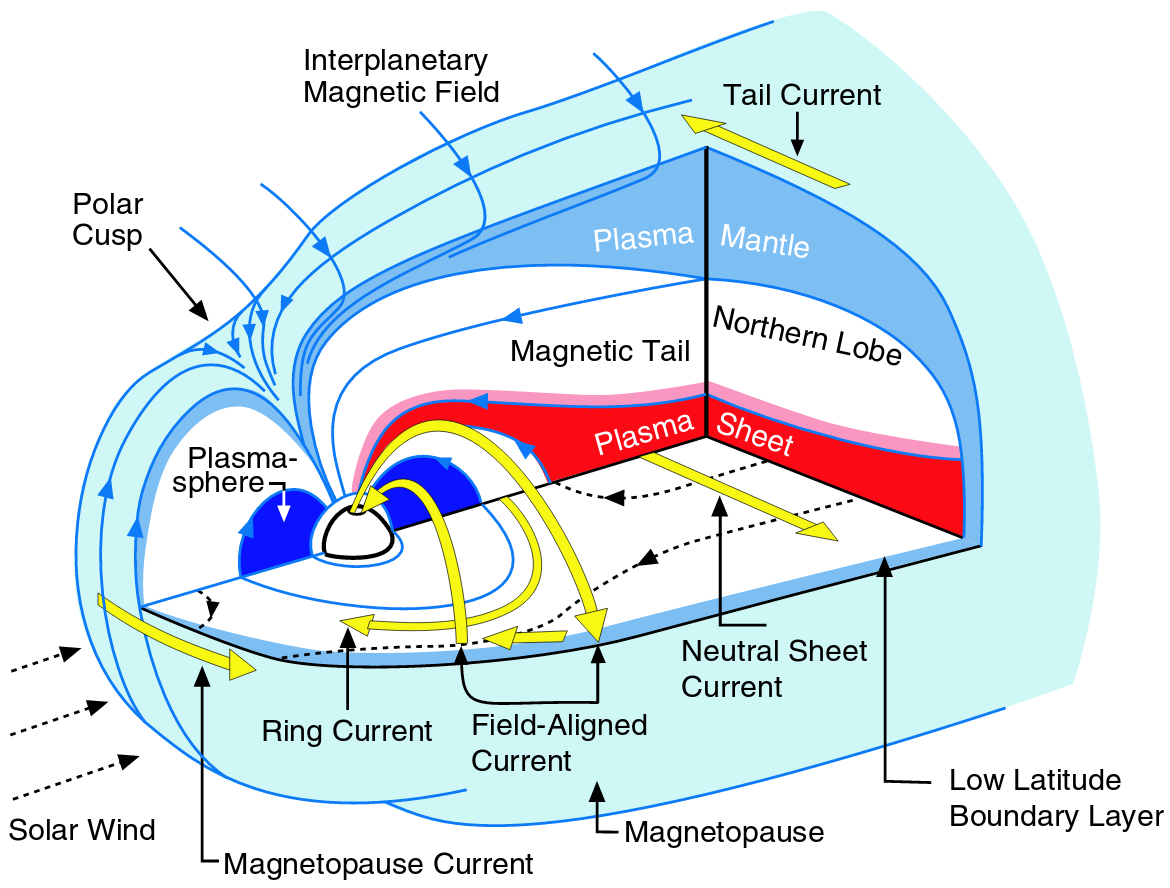
\includegraphics[width=0.6\textwidth]{figures_of_others/images/DeKeyser2005_magnetosphere.png}
	}{
		\caption[\lofimage{figures_of_others/images/DeKeyser2005_magnetosphere.png}Credit: {\citet[Fig.~2.12]{DeKeyser2005}}, adapted from {\citet[Fig.~1.18]{Kivelson1995}}, \textcopyright~Springer, reproduced with permission.]
		{Schema of the magnetosphere's inner 3D structure with focus on its current systems and plasma regions. The directions of the magnetic field lines and electric currents are indicated with blue and yellow arrows respectively. Credit: {\citet[Fig.~2.12]{DeKeyser2005}}, adapted from {\citet[Fig.~1.18]{Kivelson1995}}, \textcopyright~Springer, reproduced with permission.}
		\label{fig:DeKeyser2005_magnetosphere}
	}
\end{figure}

\pagebreak

\subsection{Solar wind coupling mechanisms}
\label{sec:solar_wind_coupling_mechanisms}
There exist several ways of how solar wind couples to the magnetosphere and deposits energy and plasma within it. The contributions of the different mechanisms by which energy is transferred and solar wind plasma is able to penetrate the magnetopause are not yet established \citep{Phan2005}. High solar wind pressure during times when the IMF direction is parallel to the terrestrial magnetic field leads to compression of the sunward magnetosphere and enhances its potential energy. Solar wind energy is also transferred via the induction of currents. However, the major interaction processes are magnetic reconnection and turbulence -- their underlying physical mechanisms are described in the following.

Magnetic reconnection occurs where the IMF comes into antiparallel contact with the terrestrial magnetic field. At these regions on the magnetopause, the magnetosphere opens up to the IMF and reconnection of the field lines occurs, resulting in a change of the local magnetic topology \citep{Phan2005}. The magnetic field reconnects along a line that shows an X"~geometry. The reconnection process at this so-called X"~line harbors a narrow diffusion region, where the plasma ions and electrons decouple to get accelerated in jets of particles by the reconnected field lines \citep{Phan2005}, see the \autoref{fig:NASA_reconnection}.
\begin{figure}[htb]
	\fcapside[\FBwidth]{
		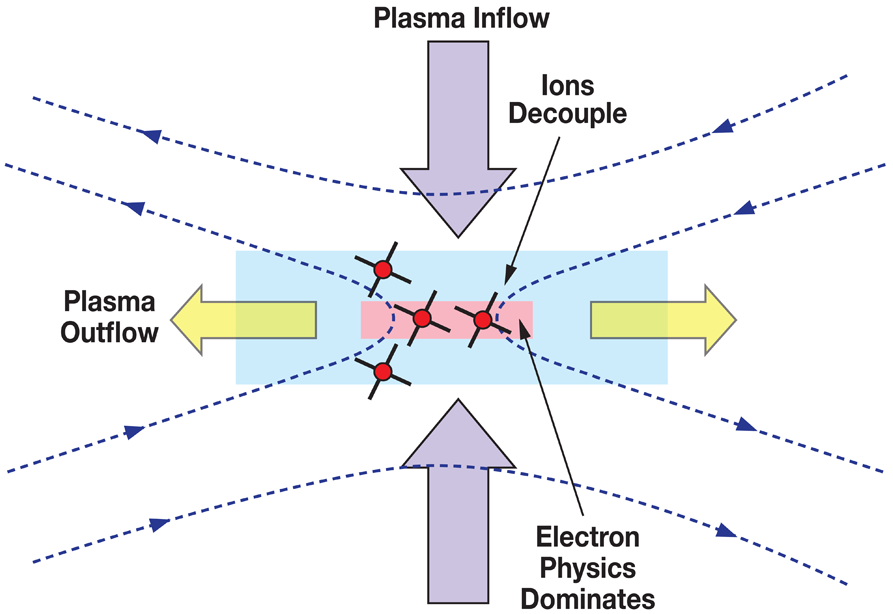
\includegraphics[width=0.5\textwidth]{figures_of_others/images/NASA_reconnection.png}
	}{
		\caption[\lofimage{figures_of_others/images/NASA_reconnection.png}Credit: \href{https://mms.gsfc.nasa.gov/science.html}{NASA/GSFC MMS mission}.]
		{Schema of an X"~line reconnection region. The dashed arrowed lines represent magnetic field lines and their direction. The large arrows indicate the plasma flow direction and the shaded areas are the ion and electron diffusion regions. The red crosses represent four Magnetospheric Multiscale (MMS) spacecraft that are built to analyze the magnetopause reconnection. Credit: \href{https://mms.gsfc.nasa.gov/science.html}{NASA/GSFC MMS mission}.}
		\label{fig:NASA_reconnection}
	}
\end{figure}
% https://mms.gsfc.nasa.gov/images/science_page/science_2_lg.png
% https://mms.gsfc.nasa.gov/science.html
Thus, the magnetopause is left with a small magnetic field normal to it, which has an opposite polarity on each side of the X"~line \citep{DeKeyser2005}.

The reconnection location on the magnetopause shifts depending on the direction of the incoming IMF as seen in \autoref{fig:Russell2007_fig4_10_VBbook_magnetopause_reconnection_regions_modified}.
\begin{figure}[b!]
	\fcapside[\FBwidth]{
		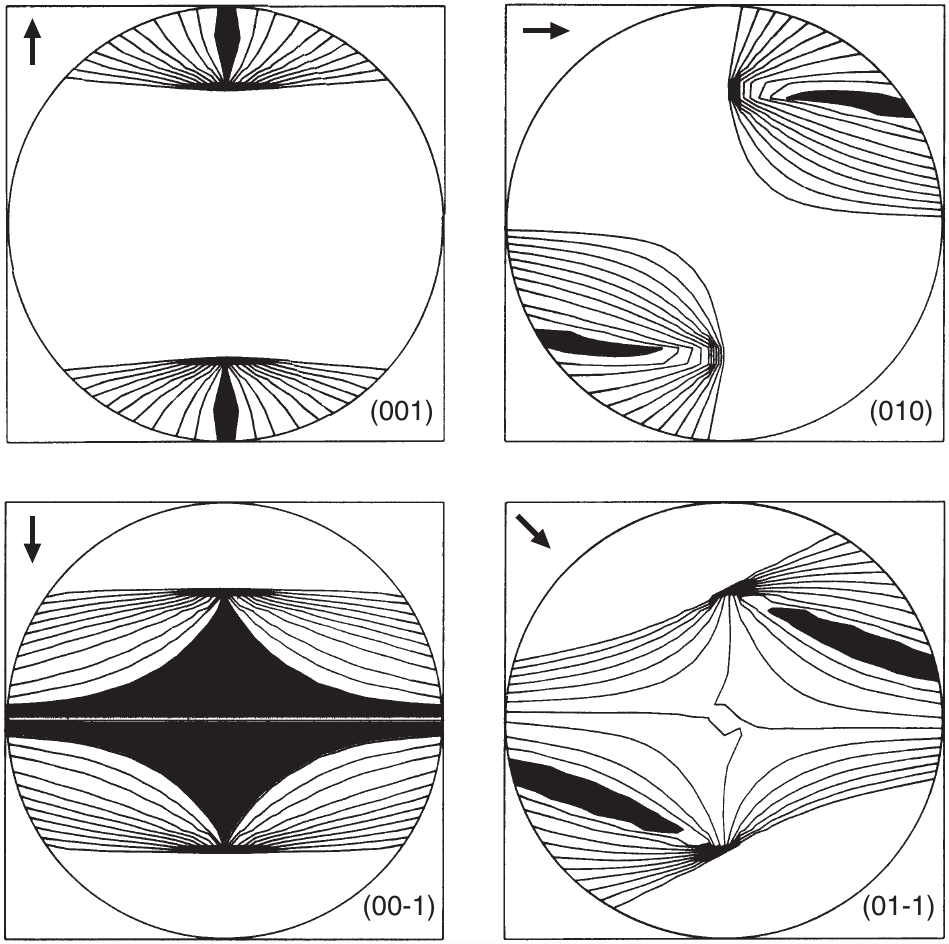
\includegraphics[width=0.6\textwidth]{figures_of_others/images/Russell2007_fig4_10_VBbook_magnetopause_reconnection_regions_modified.png}
	}{
		\caption[\lofimage{figures_of_others/images/Russell2007_fig4_10_VBbook_magnetopause_reconnection_regions.png}Credit: {\citet[Fig.~4.10]{Russell2007}}, \textcopyright~Praxis Publishing, reproduced with permission, after {\citet[Fig.~2]{Luhmann1984}}.]
		{Modeled sites of antiparallel magnetic fields (black areas) on the magnetosphere as seen from the Sun. The four different IMF directions are indicated by the arrows and indices. Credit: {\citet[Fig.~4.10]{Russell2007}}, \textcopyright~Praxis Publishing, reproduced with permission, after {\citet[Fig.~2]{Luhmann1984}}.}
		\label{fig:Russell2007_fig4_10_VBbook_magnetopause_reconnection_regions_modified}
	}
\end{figure}
During periods of southern IMF, the terrestrial field and IMF are antiparallel at the sunward point of the magnetosphere, owing to the Earth's dipole orientation. The rate of reconnection becomes highest in this case, whereas, when the IMF is directed northward, reconnection tailward of both polar cusps has been observed \citep{Phan2005}. The magnetic flux opened at the front of the magnetosphere is in average balanced by reconnections in the magnetotail, closing the field again. This process is part of the Dungey convection cycle which is described in the next \autoref{sec:dungey_convection_cycle}.
Although the microphysical processes leading to magnetic reconnection are yet little understood \citep{Phan2005}, there is evidence that magnetic reconnection is the dominant plasma transport mechanism into the magnetosphere \citep{DeKeyser2005}.

Viscous interaction with the solar wind plasma is also able to insert energy into the magnetosphere \citep{Alfven1942}. Solar wind drag at the flanks of the magnetopause creates Kelvin-Helmholtz (KH) instabilities in form of turbulent eddies. It is observed that even during northern IMF, these turbulent vortices are able to channel solar wind plasma into the magnetosphere -- either through forced magnetic reconnection (see \autoref{fig:Merkin2013_fig5_turbulence}) or non-reconnection processes \citep{Otto2003,Phan2005}. MHD simulations of the velocity shear at the magnetopause during northern IMF even suggest the presence of a double-vortex sheet structure \citep{Merkin2013}.
\begin{figure}[htb]
	\fcapside[\FBwidth]{
		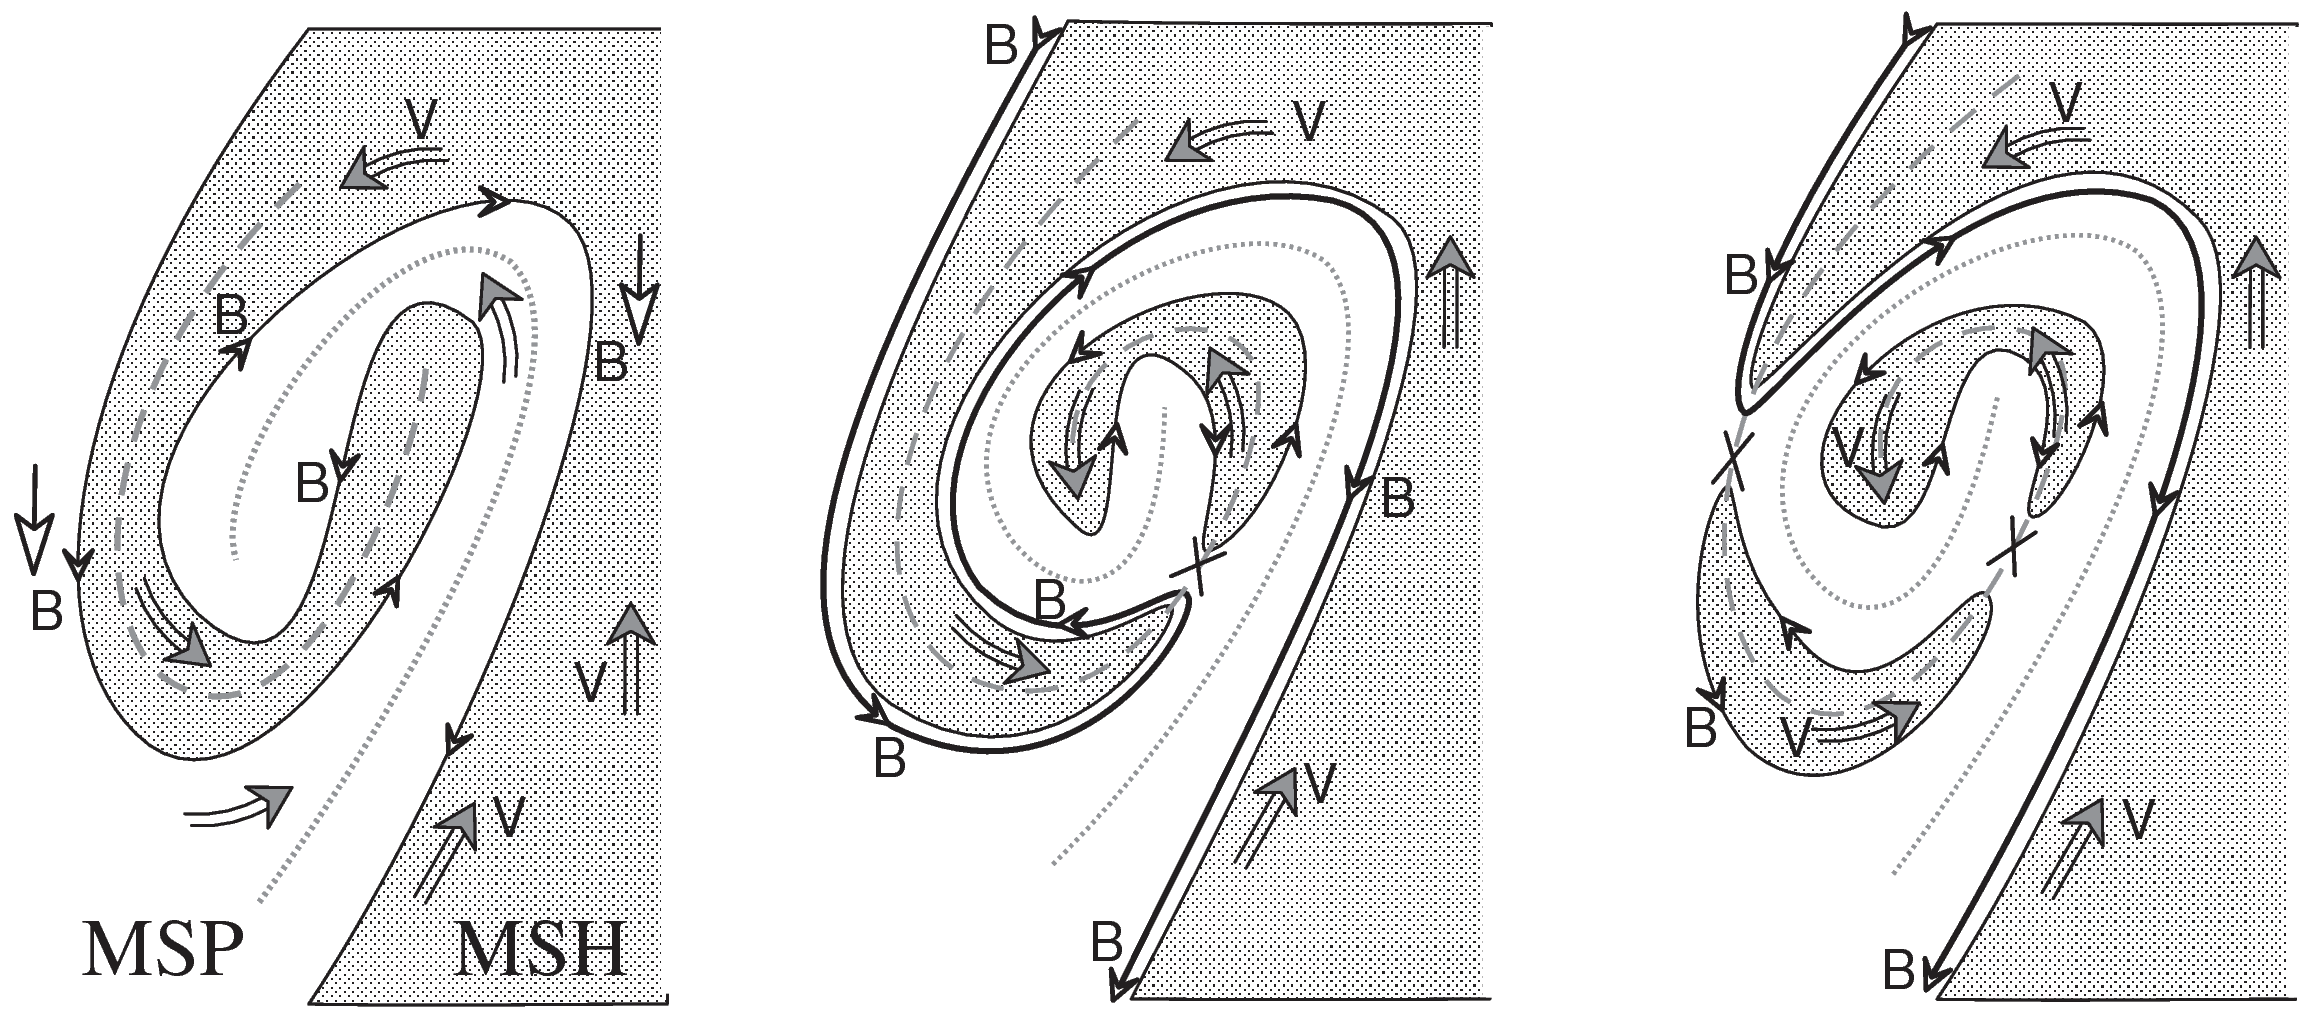
\includegraphics[width=0.6\textwidth]{figures_of_others/images/Merkin2013_fig5_turbulence.png}
	}{
		\caption[\lofimage{figures_of_others/images/Merkin2013_fig5_turbulence.png}Credit: {\citet[Fig.~5]{Merkin2013}}, \textcopyright~American Geophysical Union, reproduced with permission.]
		{Schemata showing reconnection in a turbulent vortex, forming between the magnetosphere (MSP) and the magnetosheath (MSH, shaded area) when both magnetic fields are parallel. The boundary magnetic field line is indicated by the arrowed line, the plasma flow direction by the gray arrows, and the locations of reconnection by crosses. Credit: {\citet[Fig.~5]{Merkin2013}}, \textcopyright~American Geophysical Union, reproduced with permission.}
		\label{fig:Merkin2013_fig5_turbulence}
	}
\end{figure}


\subsection{Dungey convection cycle}
\label{sec:dungey_convection_cycle}
% Dungey convection cycle
After the reconnection at the sunward magnetopause, the previously closed magnetospheric field lines are open to the IMF. They are still connected to one of Earth's magnetic poles, but their IMF part is transported by the flow of the solar wind. The field lines are stretched behind Earth and form eventually the extended magnetotail, where in its central plane reconnection recloses the field. The closed field lines migrate around the flanks of the magnetosphere to its front again, completing one magnetic convection cycle \citep{Dungey1961,Dungey1963}. The course of this so-called Dungey convection cycle, induced by the solar wind, is illustrated in \autoref{fig:Kivelson1995_fig9_11_dungey_cycle}. The Dungey cycle imprints a twin-cell convection pattern in the high latitude ionospheric plasma, where the footpoints of the geomagnetic field lines are swept from the day- to the nightside and wander back again along the lower latitudes of dusk and dawn.
\begin{figure}[htb]
	\fcapside[\FBwidth]{
		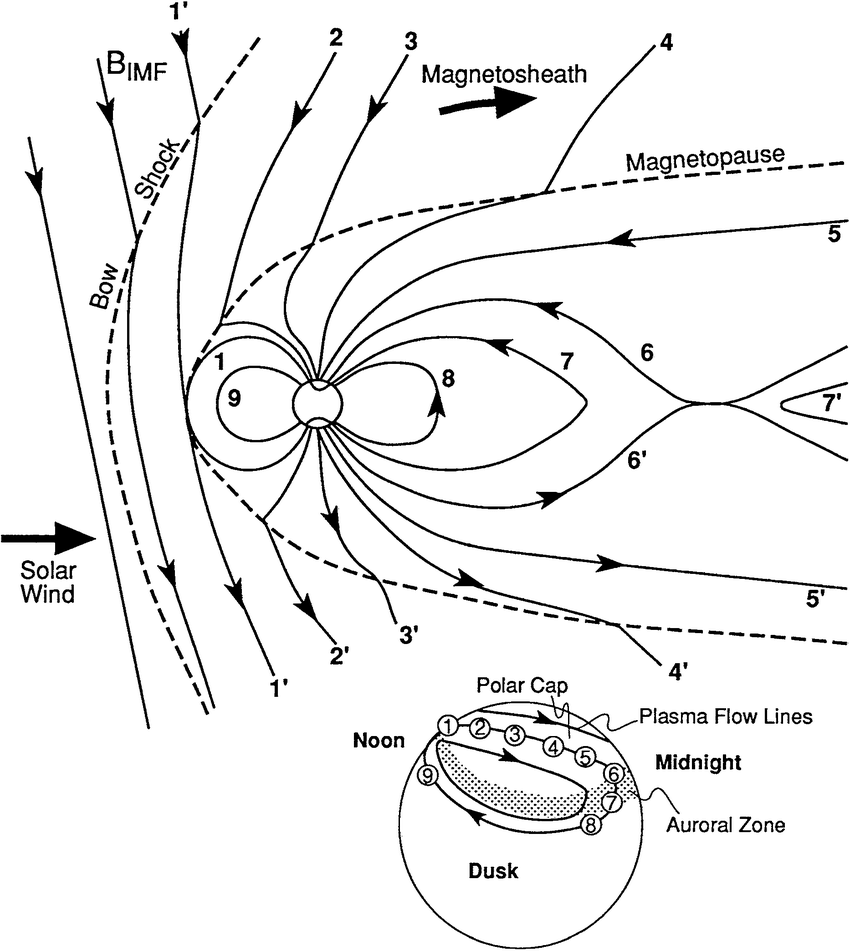
\includegraphics[width=0.55\textwidth]{figures_of_others/images/Kivelson1995_fig9_11_dungey_cycle.png}
	}{
		\caption[\lofimage{figures_of_others/images/Kivelson1995_fig9_11_dungey_cycle.png}Credit: {\citet[Fig.~9.11]{Hughes1995}}, \textcopyright~Cambridge University Press, reproduced with permission.]
		{Dungey's magnetic convection cycle illustrated in a cut through the magnetosphere (top) and on the ionosphere polar cap (bottom). The numbers on the magnetic field lines (arrowed lines) correspond to the numbered positions in the twin-cell polar cap convection cycle. Credit: {\citet[Fig.~9.11]{Hughes1995}}, \textcopyright~Cambridge University Press, reproduced with permission.}
		\label{fig:Kivelson1995_fig9_11_dungey_cycle}
	}
\end{figure}

% auroral ovals
Reconnection at the magnetopause and in the magnetotail releases and accelerates the local plasma from the reconnection site along the magnetic field lines. Thus, this plasma reaches the field lines' polar footpoints and interacts with the atoms and molecules of the upper atmosphere. This interaction, in particular between electrons from the magnetotail and atmospheric oxygen/nitrogen, creates the aurorae. The auroral ovals are located at the boundaries between the closed terrestrial field and the field open to the IMF. The open field regions, enclosed by the auroral ovals, are the polar caps. The increased reconnection during southward IMF erodes the magnetopause \citep{Aubry1970}, shifting the auroral ovals to lower latitudes. Likewise, the azimuthal IMF component shifts the auroral oval towards dawn or dusk.

The Dungey cycle is not a steady-state process, that is, the rates of opened and reclosed terrestrial magnetic flux are equal only in the long term. The dayside opening flux rate $\Phi_\text{D}$ is modulated by the dynamic behavior of the solar wind and the orientation of the IMF, whereas the nightside closing flux rate $\Phi_\text{N}$ depends on the situation in the magnetotail \citep{Milan2007}, see \autoref{fig:Milan2009_magnetosphere}.
\begin{figure}[htb]
	\fcapside[\FBwidth]{
		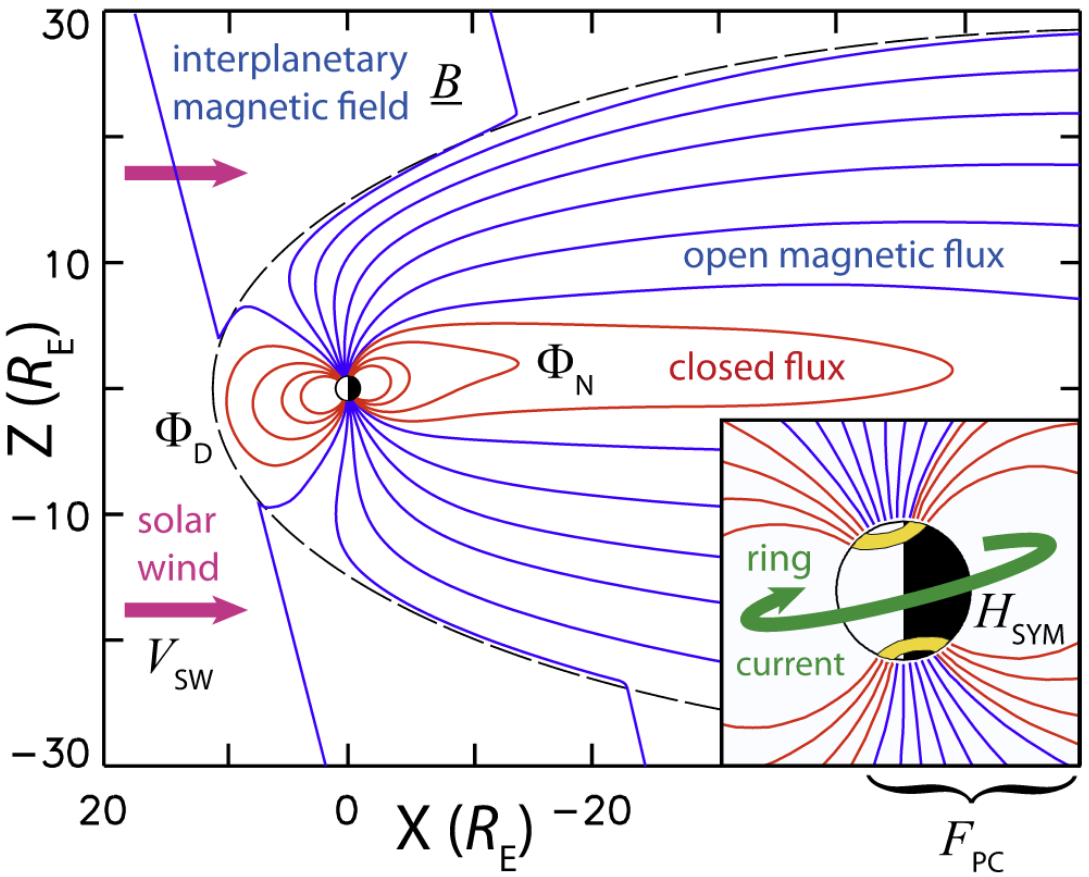
\includegraphics[width=0.6\textwidth]{figures_of_others/images/Milan2009_magnetosphere.png}
	}{
		\caption[\lofimage{figures_of_others/images/Milan2009_magnetosphere.png}Credit: {\citet[Fig.~1]{Milan2009}}, \textcopyright~American Geophysical Union, reproduced with permission.]
		{Schema of the magnetosphere for the case of southern IMF direction with emphasis on open (blue lines) and closed (red lines) magnetic flux. The magnetopause is indicated by the dashed line. The opening flux rate at the dayside is denoted with $\Phi_\text{D}$ and the closing flux rate at the nightside with $\Phi_\text{N}$. The inset shows day- and nightside of Earth and the relation between auroral ovals (yellow areas) and the open flux at the polar caps ($F_\text{PC}$). The ring current intensity $H_\text{SYM}$ and direction (green arrow) are plotted as well. Credit: {\citet[Fig.~1]{Milan2009}}, \textcopyright~American Geophysical Union, reproduced with permission.}
		\label{fig:Milan2009_magnetosphere}
	}
\end{figure}
The propagation time of the solar wind from the sunward magnetopause to the magnetotail amounts to a lag of about half an hour. Thus, because the rate of reconnection scales with the changing dynamic pressure of the solar wind, the total amount of open flux $F_\text{PC}$ varies with time so that the ionospheric polar caps expand/contract with time as well \citep{Siscoe1985}:
\begin{align}
	\frac{\text{d}F_\text{PC}(t)}{\text{d}t} = \Phi_\text{D}(t) - \Phi_\text{N}(t)	\,.	\label{eq:faradays_law}
\end{align}
Continuous reconnection on the sunward magnetopause builds up the polar cap flux and thus increases stress in the magnetotail, which leads there to regular reconnection bursts, releasing the flux again.

% magnetopause reconnection
During sunward reconnection, the magnetic field component normal to the magnetopause undergoes regular bipolar oscillations that are interpreted as temporary reconnection events, transferring magnetic flux to the magnetotail. These flux transfer events occur with a period of about eight minutes \citep{Russell1996}. When solar wind conditions are steady, the reconnection process at the sunward magnetopause is found to be steady as well \citep{Phan2005}. During changing IMF direction, the reconnection site moves and intermittent reconnection has been locally observed, but the overall reconnection keeps being continuous and never ceases \citep{Phan2005}.

% tail reconnection/substorms
The reconnection in the magnetotail occurs in regular intermittent reconnection bursts. These bursts can produce magnetic plasmoids that release from the tail and are swept away with the solar wind. This pulsed reconnection has a period of a few hours and is the major nightside flux closure process \citep{Milan2007}. The subsequent effects on the magnetospheric field are called substorms. Their duration varies greatly around an average value of 70~minutes and they vary in intensity as well. Substorms create sudden brightenings and increased activity in the aurora, which also show characteristic patterns matching the substorm cycle. Substorms are found to occur spontaneously during southward IMF periods, however, in \SI{60}{\percent} of the cases they are triggered by changing upstream solar wind conditions -- either by switches in the IMF orientation or by shocks in the solar wind ram pressure \citep{Milan2007}.
The arrival of extreme solar wind conditions, such as found in CMEs and CIRs, generates geomagnetic disturbances larger than substorms, these geomagnetic storms are described in \autoref{sec:geomagnetic_storms}.

\clearpage

\subsection{Russell-McPherron effect}
\label{sec:russell_mcpherron_effect}
Geomagnetic activity varies semiannually with the maxima around the equinoxes and the minima around solstices \citep{Cortie1912}. \citet{Russell1973} suggested a model, now called the Russell-McPherron (R-M) effect, that is able to predict the correct phase and the observed variation in strength seen yearly in geomagnetic activity. They defined a solar wind-magnetosphere interaction in GSM coordinates that is set to zero during northward IMF and is otherwise proportional to the southward IMF component -- analog to a half-wave rectifier. As solar wind and IMF are naturally ordered in the geocentric solar equatorial (GSEQ) coordinate system, their flow angle against the magnetosphere undergoes seasonal variations. The R-M effect then is provided by the changing probability over the year of a north- or southward IMF, viewed in the GSM-frame of the magnetosphere. This variation is found to be sufficient to generate the observed effect \citep{Russell1973}.
There exist other hypotheses describing the semiannual variation: the axial and the equinoctial hypotheses. However, the R-M effect is the most prevailing and is even able to explain the changes in geomagnetic activity under extreme solar wind conditions, such as interplanetary shocks \citep{Zhao2012}.

In addition to the R-M effect, the interaction depends on the dipole tilt angle to the solar wind, which is shown to regulate the extent of the sunward reconnection region and therefore the reconnection rate and geomagnetic activity \citep{Russell2003}.


\subsection{Geomagnetic indices}
\label{sec:geomagnetic_indices}
In order to monitor the state of the magnetospheric system and disturbances therein, geomagnetic observatories are widely distributed over the globe, measuring the local magnetic field at their position. Magnetic measurements from several sets of stations define several geomagnetic indices. The measurements cover specific regions in order to monitor the state of different parts of the magnetospheric system. The major global geomagnetic indices are supported by the International Association of Geomagnetism and Aeronomy (IAGA) and serviced by the International Service of Geomagnetic Indices (ISGI)\footnote{ISGI website: \urlfoot{http://isgi.unistra.fr/}}. These indices and their purpose are listed in the following: The $aa$~index is designed to represent the amplitude of the global geomagnetic activity, normalized to a geomagnetic latitude of \SI{+-50}{\degree}. The $am$~index characterizes the global geomagnetic activity. The \Kp{}~index is designed to measure geomagnetic disturbances from solar particle radiation. The $Dst$~index monitors the intensity of the magnetospheric ring current. The $PC$~index monitors the polar cap magnetic activity -- it approximates the amount of energy which entered the magnetosphere through solar wind coupling. The $AE$~index and its relatives $AU$, $AL$ and $AO$ measure the magnetic effects of the northern auroral electrojet. The first three listed indices ($aa$, $am$ and \Kp{}) are calculated from different sets of local 3"~hourly $K$~indices, which measure the local magnetic disturbances at the observatories.	% There exist several sub-indices that are based on some of those listed above, e.g., ap, Ap, Cp, C9, Aa, Kpa, an, as, Kpm, Am, An, and As.\\
The \Kp{} and $Dst$~indices are described in more detail in the following section.


\section{Geomagnetic storms}
\label{sec:geomagnetic_storms}
% difference to substorms
Geomagnetic storms are major disturbances in the geomagnetic field, generated under extreme solar wind conditions. In contrast to substorms which originate in the magnetotail, geomagnetic storms are directly caused by the incoming solar wind flow at the sunward magnetopause. Indeed, the main phase of geomagnetic storms is always accompanied in parallel by substorms \citep{Gonzalez1994}. During geomagnetic storms, substorms even occur in higher frequencies and can overlap each other.

% caused by solar wind structures
\citet{Carrington1859} was the first to associate a geomagnetic storm with an event of solar origin, that is, he noticed a major solar flare appearing a few hours before the storm. The corresponding solar event is known as the Carrington event, as the resulting geomagnetic storm is the largest ever observed. \citet{Forbush1937} found a rapid reduction in cosmic-ray intensity occurring parallel to a geomagnetic storm, now known as 'Forbush decreases', and attributed both to a common external cause. Eventually, \citet{Wilson1987} demonstrated the connection between geomagnetic storms and MCs by finding simultaneous decreases in the $Dst$~index during episodes of southward IMF within MCs. The order in which north- and southward IMF appears in an MC does not matter for the final observed $Dst$ magnitude, unless part of the MC is compressed, but the $Dst$ activity is always in phase with the southward field \citep{Zhang1988}. Finally, \citet{Gosling1993} established that CMEs rather than flares are the main cause of major geomagnetic storms and large SEP events. Indeed, single and multiple CME events are found to be the most geoeffective solar wind structures in that they are accountable for about \SI{87}{\%} of the major geomagnetic storms, whereas the remainder is produced by CIR events \citep{Bothmer1995,Zhang2007}.

Solar wind injects plasma and energy into the magnetosphere, varying the number of particles in the magnetospheric equatorial current system, the so-called ring current, illustrated in Figures~\ref{fig:DeKeyser2005_magnetosphere} and~\ref{fig:Milan2009_magnetosphere}. The ring current is located between \SIrange{2}{7}{\RE} \citep{Gonzalez1994}. When the ring current is increased due to incoming CMEs or CIRs, it generates an enhanced magnetic field of opposite polarity to the magnetospheric field. This leads to a decrease in the local terrestrial magnetic field.

% Dst index
The decrease is measured by four magnetic observatories located near the dipole equator. Their magnetic field measurements are the base for the disturbance storm time index $Dst$ \citep{Sugiura1991}. Therefore, $Dst$ represents the intensity of the ring current and is a quantitative measure for geomagnetic disturbances. The $Dst$~index is derived and published through the IAGA at the World Data Center for Geomagnetism in Kyoto\footnote{WDC for Geomagnetism, Kyoto; $Dst$~index service: \urlfoot{http://wdc.kugi.kyoto-u.ac.jp/dstdir/index.html}}.

Historically, the size of a geomagnetic storm was defined as the peak negative disturbance in the $Dst$~index. Though, the onset of a geomagnetic storm is typically an abrupt increase in $Dst$, referred to as a storm sudden commencement (SSC). The initial period of positive $Dst$ lasts several hours and is caused by the compression of the magnetosphere due to the increased pressure of arriving shocked solar wind plasma. The intensity of a geomagnetic storm can be gauged by the minimum $Dst$ that is reached in its main phase -- during moderate storms $Dst$ falls below \SI{-50}{\nano\tesla} and during intense storms below \SI{-100}{\nano\tesla} \citep{Gonzalez1994}. The main phase lasts a few hours, but the recovery to average $Dst$ levels is gradual and can take up to several days.

% Kp index
However, as $Dst$ only shows disturbances in the ring current intensity, another index has been used more widely for the assessment of planetary geomagnetic activity, the \Kp~index \citep{Gonzalez1994}. \Kp{} is now the most prevalent index used by space weather forecasters to indicate the severity of geomagnetic storms \citep{Wing2005}, for instance, \Kp{} is the basis for NOAA's G"~Scale\footnote{NOAA Space Weather Scales website: \urlfoot{https://www.swpc.noaa.gov/noaa-scales-explanation}}.

Field-aligned currents, called Birkeland currents, connect ionospheric currents located in the nightside auroral oval, called the auroral electrojets, to the magnetopause and the partial ring current \citep{Coxon2014}, see \autoref{fig:DeKeyser2005_magnetosphere}. In addition to the ring current, this current system generates large magnetic disturbances as well. Collectively, all currents contribute to the planetary geomagnetic disturbances, which are quantified on the ground with the planetary geomagnetic disturbance index \Kp{}.


\subsection{\Kp{}~index}
\label{sec:kp_index}
Julius~Bartels introduced a \textit{K}~index in 1938 and designed it to measure the intensity of geomagnetic disturbances \citep{Bartels1939}. Its name originates from 'Kennziffer' -- the German word for characteristic digit. The \textit{K}~index is a measure for the maximal variation of the surface magnetic field, observed in a magnetogram within 3"~hour intervals. Its scale in the range 0--9 is a quasi-logarithmic representation of the actual magnetic field strength's variations.

The Planetary \textit{K}~index (\Kp{}) is a planetary geomagnetic disturbance index, introduced by Bartels in 1949 at the Institute for Geophysics, University of Göttingen \citep{Bartels1949}. \Kp{} is the weighted average of 13 \textit{Ks}~indices, which are the standardized versions of the local \textit{K} indices measured at 13 observatories. These contributing observatories are located around \SI{+-50}{\degree} geomagnetic latitude and their distribution is biased towards Europe, as can be seen in the map in \autoref{fig:Kp_map}.
\begin{figure}[htb]
	\fcapside[\FBwidth]{
		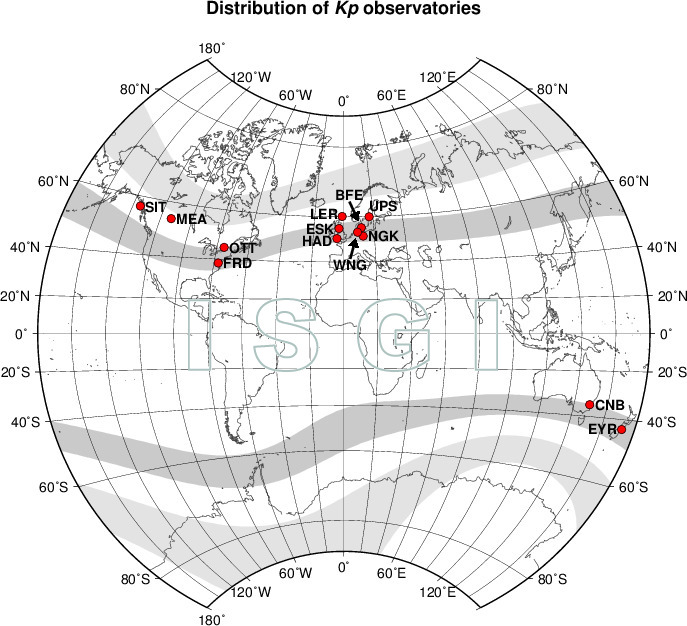
\includegraphics[width=0.55\textwidth]{figures_of_others/images/Kp_map.jpg}
	}{
		\caption[\lofimage{figures_of_others/images/Kp_map.jpg}Courtesy of \href{http://isgi.unistra.fr/indices_kp.php}{International Service of Geomagnetic Indices (ISGI)}, 2013.]
		{Distribution of the 13 \Kp{} observatories. The shaded belts indicate regions of equal geomagnetic latitude. Courtesy of \href{http://isgi.unistra.fr/indices_kp.php}{International Service of Geomagnetic Indices (ISGI)}, 2013.}
		\label{fig:Kp_map}
	}
\end{figure}
% contacted via email: got permission
%\urlfoot{http://isgi.unistra.fr/indices_kp.php}
To benefit from its higher precision, its scale, in the range 0--9 as well, is further divided into thirds, represented by the suffixes '$+$', 'o' and '$-$' (e.g., 3o, $3+$, $4-$, 4o). The \Kp{}~indices are often visualized in musical diagrams, where they are stacked into periods of 27~days to enable the detection of recurrent geomagnetic activity, as seen in \autoref{fig:musi1612}.

The \Kp{}~index can be converted to the 3"~hour equivalent \textit{ap}~index, which represents the magnetic field strength at a surface position of about \SI{+-50}{\degree} dipole latitude. The conversion is done via a table specified by Bartels, in which the value of the \textit{ap}~index is scaled in units of \SI{2}{nT}, as seen in \autoref{tab:kp_to_ap_table}.
\begin{table}[h!]
	\caption{Table for the fixed conversion from the \Kp~index to the equivalent \textit{ap}~index, which represents the magnetic field strength in units of \SI{2}{nT}.}
	\label{tab:kp_to_ap_table}
	\centering
	\begin{tabular}{lssssssssssssss}
		\Kp	&0o	&0+	&1-	&1o	&1+	&2-	&2o	&2+	&3-	&3o	&3+	&4-	&4o	&4+\\
		\textit{ap}	&0	&2	&3	&4	&5	&6	&7	&9	&12	&15	&18	&22	&27	&32\\
		\hline
		\Kp	&5-	&5o	&5+	&6-	&6o	&6+	&7-	&7o	&7+	&8-	&8o	&8+	&9-	&9o\\
		\textit{ap}	&39	&48	&56	&67	&80	&94	&111	&132	&154	&179	&207	&236	&300	&400
	\end{tabular}
\end{table}
\pagebreak
There are further geomagnetic indices which are derived from the \Kp{}~index. They include $Ap$, the daily \textit{ap} average, $Cp$, the daily \textit{ap} sum mapped via a fixed table to the range \numrange{0}{2.5}, and $C9$, a mapping of $Cp$ via a fixed table to the range \numrange{0}{9}. The definitions of Q"~days (quiet days) and D"~days (disturbed days) are also obtained from the \Kp{}~index.

The IAGA adopted the \Kp{}~index in 1954. The \Kp{}~index was maintained in Göttingen until January 1997 -- now the German Research Centre for Geosciences (GFZ) in Potsdam supplies the \Kp{}~index and thereof derived indices. See also the \Kp{} data description in \autoref{sec:kp_data}.

\begin{figure}[htb]
	\centering
	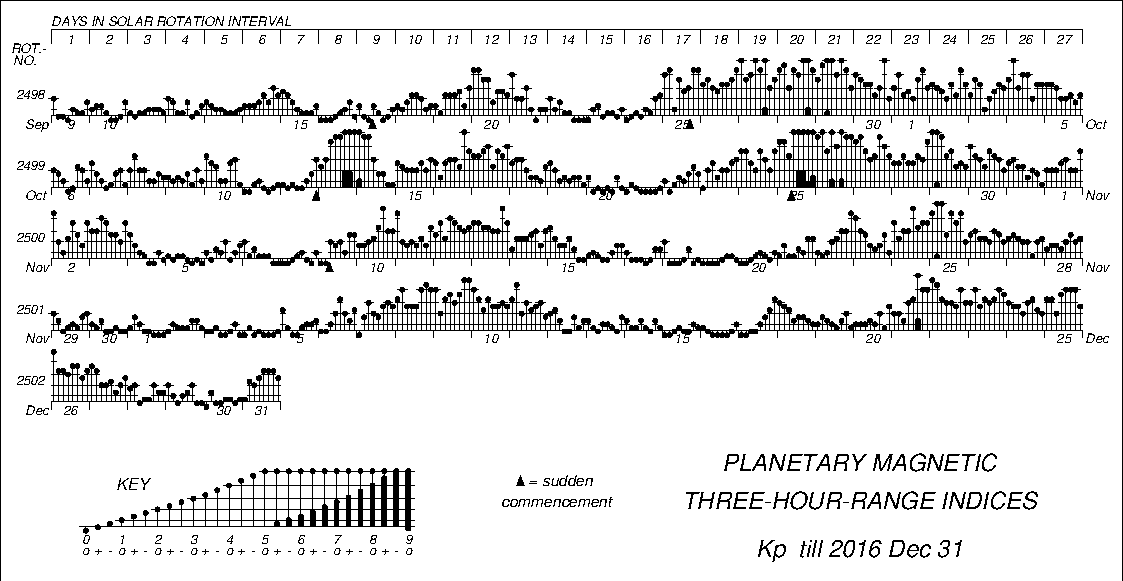
\includegraphics[width=\textwidth]{figures_of_others/images/musi1612.pdf}
	\caption[\lofimage{figures_of_others/images/musi1612.pdf}Credit: \href{http://www.gfz-potsdam.de/en/kp-index/}{GFZ~Potsdam}, 2017, licensed under \href{https://creativecommons.org/licenses/by/4.0/}{CC BY 4.0}.]
	{Bartels musical \Kp{} diagram for the time period from September until end of December 2016. Two sudden commencements with following geomagnetic storms, having a maximal \Kp{} of $6+$, can be seen in October. Credit: \href{http://www.gfz-potsdam.de/en/kp-index/}{GFZ~Potsdam}, 2017, licensed under \href{https://creativecommons.org/licenses/by/4.0/}{CC BY 4.0}.}
	\label{fig:musi1612}
\end{figure}
%ftp://ftp.gfz-potsdam.de/pub/home/obs/kp-ap/music/

\clearpage

\section{Geomagnetic activity forecast}
\label{sec:geomagnetic_activity_forecast}
The timing and intensity of geomagnetic storms is sought to be forecasted from knowledge about the upcoming solar wind conditions. This means that there are two questions to this task: First, how does the incoming magnetized solar wind plasma result in magnetospheric disturbances? In order to resolve this, coupling functions relating geomagnetic indices to solar wind parameters are essential. Second, what state will the arriving solar wind be in at the magnetopause? Hence, a forecast using remote observations is required which is able to predict the arrival time and conditions of solar wind streams and CMEs. Both topics are addressed in the following subsections.


\subsection{Coupling functions}
\label{sec:coupling_functions}
In order to quantify geomagnetic activity, solar wind coupling functions that correlate sufficiently well with geomagnetic indices are necessary. These relations can then be used to connect solar wind parameters with geomagnetic indices via empirically fitted functions, as is described for the \Kp~index at the end of this section.

% merging and viscous functions
The major interaction mechanisms between solar wind and magnetosphere are magnetic reconnection and viscous turbulence, as mentioned previously in \autoref{sec:solar_wind_coupling_mechanisms}. \citet{Newell2008} found recently that coupling functions show the highest correlation when they consist of a merging term combined with a viscous term.
% merging functions
The rate magnetic flux merges with the IMF (i.e., is opened at the magnetopause) generally depends on the following independent factors \citep{Newell2007}:
\begin{itemize*}
	\item The rate magnetic flux is transported towards the magnetopause, represented by the solar wind velocity.
	\item The amount of opened flux, which scales with the IMF strength.
	\item The merging probability, which depends on the IMF clock angle.
	\item The extent of the reconnection region, represented by the length of the X"~line on the magnetopause.
\end{itemize*}
As the viscous term describes another kind of interaction process, that is, reconnections due to Kelvin-Helm\-holtz instabilities at the flanks of the magnetosphere, it is independent from the dayside reconnection term. The viscous term accounts for the smaller fraction of variance and depends on the solar wind plasma quantities velocity and density \citep{Newell2008}.

Many coupling functions were proposed in order to characterize the solar wind's interaction processes with the magnetosphere. They consist of functional terms of differing complexity, mostly including and approximating several of the factors listed above. There exist a lot of coupling functions based on combinations of the same physical quantities, often including the IMF direction \citep{Newell2007,Lockwood2013}. Here I list and discuss a few of the most used coupling factors and functions:
\begin{itemize}
	\item $v$, the solar wind velocity. At an early stage, \citet{Snyder1963} found a strong correlation of the daily average velocity with geomagnetic activity from Mariner~2 solar wind measurements.
	
	\item $B_\text{z}$, the IMF z"~component. \citet{Fairfield1966} deduced from early satellite IMF measurements that a southward IMF direction is linked with geomagnetic disturbances, whereas a northward is connected with quiet geomagnetic conditions. For this purpose it makes sense to use the geocentric solar magnetospheric (GSM) coordinate system, which is aligned with the Earth's magnetic dipole axis.
	
	\item $B_\text{s}$, the half-wave rectifier as defined by \citet{Russell1973}, see also the R-M effect in \autoref{sec:russell_mcpherron_effect}. It describes a simple interaction in GSM coordinates that is proportional to the southward IMF component and zero during northward IMF:
	\begin{align}
		B_\text{s} =
		\begin{cases}
			\,0 &\text{for } B_\text{z} > 0	\,,\\
			\,-B_\text{z} &\text{for } B_\text{z} \le 0	\,.
		\end{cases}	\label{eq:half_wave_rectifier}
	\end{align}
	
	\item $B$, the absolute IMF magnitude. The long-term average IMF strength is observed to be proportional to the level of geomagnetic activity \citep{Stamper1999,Lockwood2013}. This is due to the fact that the IMF orientation is averaged out on yearly timescales and the average southward IMF component becomes proportional to $B$.
	
	\item $|\vect{B}| \sin^n\left(\theta_c / 2\right)$, a term depending on the IMF clock angle $\theta_c$ and in shape similar to the half-wave rectifier. However, it is continuous around zero and therefore often preferred over $B_\text{s}$ \citep{Lockwood2013}. The IMF clock angle is defined as $\theta_c = \tan^{-1}\left(B_\text{y} / B_\text{z}\right)$ and the exponent $n$ is often chosen to be between 2 and 4, see also \autoref{fig:coupling_angle_f}. The term stands for the fraction of IMF field lines which merge with the magnetopause, that is, the merging probability of those IMF field lines which impact the magnetopause.
	\begin{figure}[htb]
		\fcapside[\FBwidth]{
			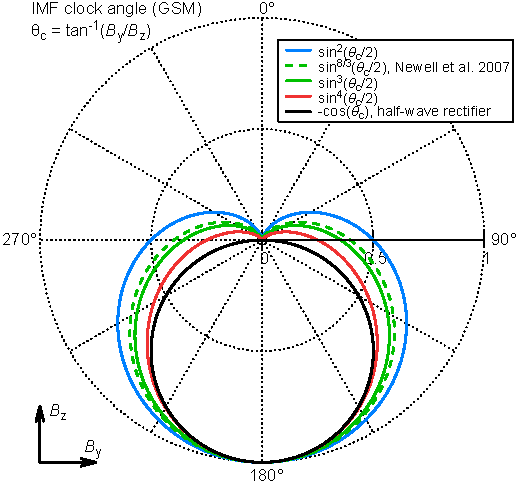
\includegraphics[width=0.6\textwidth]{figures_of_mine/gnuplots/coupling_angle_f.pdf}
		}{
			\caption[\lofimage{figures_of_mine/gnuplots/coupling_angle_f.pdf}I created the figure myself.]
			{IMF clock angle dependency of the coupling functions' relative amplitudes. The different functions include the IMF clock angle factor by \citet{Newell2007} and the half-wave rectifier. I also added the GSM coordinate directions in the lower left for orientation.}
			\label{fig:coupling_angle_f}
		}
	\end{figure}
	
	\item $\vect{E}$, the solar wind electric field which is, with the help of several assumptions, often reduced to part of its y"~component:
	\begin{align}
		\vect{E} &= -\vect{v} \times \vect{B}	\,,\\
			&\approx E_\text{y} \approx -v_\text{x} B_\text{z}	\,.	\label{eq:coupling_vxBz}
	\end{align}
	It is one of the most prominent coupling functions and simply represents the rate at which north- and southward magnetic flux is transported to the magnetosphere \citep[p.~103]{Russell2007}. How this relation is derived and which assumptions are made for the reduction to $E_\text{y}$ is described in the Appendix~\ref{sec:electric_field_at_the_magnetopause}.
	
	\item $\varepsilon$, the epsilon parameter which is based on the solar wind's energy density \citep{Perreault1978}. It represents the Poynting flux entering the magnetosphere:
	\begin{align}
		\varepsilon \propto {l_0}^2 v B^2 \sin^4\left(\frac{\theta_c}{2}\right)	\,,
	\end{align}
	where $l_0$ is a scaling factor for the cross-sectional area of the magnetosphere.
	
	\item $P_\alpha$, the solar wind power coupled into the magnetosphere \citep{Stamper1999,Lockwood2013}. It consists of the product of the solar wind power density, the cross sectional area of the magnetosphere, and the fraction of the incident power that crosses the magnetopause:
	\begin{align}
		P_\alpha \propto n^{2/3 - \alpha} v^{7/3 - 2 \alpha} B^{2 \alpha} \sin^4\left(\frac{\theta_c}{2}\right)	\,.
	\end{align}
	The coupling exponent $\alpha$ depends on the coupling to the solar wind Alfvén Mach number and has a value around 0.4.

	\item $\Phi_\text{A}$, the Boyle index, which represents the steady state asymptotic polar cap potential drop \citep{Boyle1997}:
	\begin{align}
		\Phi_\text{A} = \num{1.01e-4} v^2 + 11.7\,|\vect{B}| \sin^{3}\left(\frac{\theta_c}{2}\right)	\,,
	\end{align}
	measured in \si{\kilo\volt} with the velocity in \si{\km\per\s} and the magnetic field in \si{\nano\tesla}. \citet{Boyle1997} note that the viscous $v^2$ dependence is better represented by an additional term rather than being a modulation of the latter merging term.
	
	\pagebreak
	
	\item $\text{d}\Phi / \text{d}t$, a relation derived by \citet{Newell2007}. It represents the rate magnetic flux is opened at the magnetopause:
	\begin{align}
		\frac{\text{d}\Phi}{\text{d}t} &= v^{4/3} |\vect{B}|^{2/3} \sin^{8/3}\left(\frac{\theta_c}{2}\right)	\,.	\label{eq:newell_merging_function}
	\end{align}
	The X"~line length is approximated with $\left(v / |\vect{B}|\right)^{1/3}$ and is included within the first two factors. The value of the sine exponent, $n = 8/3$, is determined empirically. This relation shows the highest correlation with 9 out of 10 geomagnetic indices out of a number of tested coupling functions, aiming to be an universal solar wind-magnetosphere coupling function \citep{Newell2007}. The coupling function's correlation coefficient with the \Kp~index reaches a value of $r = 0.760$.
	
	\item \citet{Newell2008} found that a single coupling function, consisting of a merging and a viscous part, is able to describe the solar wind-magnetosphere interaction best, in that it correlates with the behavior of a broad range of geomagnetic indices. One of the best combinations for the \Kp~index is the merging term $\text{d}\Phi / \text{d}t$ together with the viscous term $\sqrt{n} \cdot v^2$, resulting in a correlation coefficient as high as $r = 0.866$.
	
\end{itemize}


\subsection{\Kp{} forecast methods}
% Kp empirical functions
However, the correlation of a coupling function only shows which quantities are involved in the interaction and how much they contribute to the observed variance. In order to quantify the interaction and relate the coupling functions to geomagnetic indices, empirical relations are obtained by fitting the mutual distribution of both time series.

As the \Kp~index is the measure for the size of geomagnetic disturbances, many simple and more complex analytical functions connecting \Kp{} with different solar wind coupling functions were derived. For instance, \citet{Snyder1963} deduced the following velocity relation for the daily sum of the eight \Kp{} values from Mariner~2 data: $\sum \Kp(v) = (v - 330) / 8.44$. Another example is the relation developed by \citet{Newell2008}, comprising the previously mentioned coupling function set of a merging and a viscous term. Their equation for the least variance linear prediction of \Kp{} is
\begin{align}
	\Kp{} = 0.05 + \num{2.244e-4} \frac{\text{d}\Phi}{\text{d}t} + \num{2.844e-6} \sqrt{n} \cdot v^2	\,.
\end{align}
Whereas, \citet{Mays2015} fitted only $\text{d}\Phi / \text{d}t$ with the \Kp~index and obtained the empirical relation
\begin{align}
	\Kp = 9.5 - \exp\left(2.18 - \num{5.20e5} \left(\frac{\text{d}\Phi}{\text{d}t}\right)\right)	\,,
\end{align}
with the velocity measured in \si{\km\per\s} and the magnetic field in \si{\nano\tesla}.

% Kp now- and forecast
The different empirical functions are utilized within various models developed for predicting the \Kp~index in advance. Their prediction times range from simple nowcasts to forecasts of a few days, depending on the type of input data. The input can be solar wind real-time measurements made right ahead of Earth at L1, just as stream/CME arrival predictions derived from remote observations of the solar surface and corona. These two input sources are outlined in the next section.
Another sophisticated prediction method relies on artificial neural networks. Models utilizing this method usually rank highest in prediction performance.
Below I list a few currently existing operational services that implement various \Kp{} prediction methods, including nowcasts, forecasts, and manual warnings:
\begin{itemize}
	\item The GFZ German Research Centre for Geosciences Potsdam is the responsible institution for releasing the official \Kp{}~index. Additionally, it also calculates a nowcast \Kp~index from the already available magnetic observations. The Nowcast \Kp~index is provided at the website of the GFZ~Potsdam:\\
	\urltext{https://www.gfz-potsdam.de/en/kp-index/}
	
	\item NOAA's Space Weather Prediction Center (SWPC) provides an estimated \Kp~index using ground-based real-time magnetometer measurements from a set of eight international observatories. The Planetary $K$"~index nowcast is available at the SWPC:\\
	\urltext{https://www.swpc.noaa.gov/products/planetary-k-index}
	
	\item The Wing APL models provide 1- and 4"~hour \Kp{} predictions. They are based on neural network models that take as input the solar wind real-time measurements made at L1 and the current \Kp{} nowcast \citep{Wing2005}. The Wing \Kp{} models are provided by the U.S. Air Force Weather Agency and were hosted on the website of the SWPC until 27~June 2018\footnote{SWPC page removal notice: \href{https://www.swpc.noaa.gov/news/usaf-wing-kp-model-removed-swpc-website}{USAF Wing Kp model removed from SWPC website}}.
% 	\texttt{https://www.swpc.noaa.gov/products/wing-kp}
	
	\item \citet{Bala2012} developed \Kp{} prediction models that offer 1- and 3"~hour forecast times. Their models are also based on artificial neural networks that use real-time solar wind measurements. They utilize the Boyle index, an empirical approximation for the polar cap potential, as a coupling function. The model predictions can be accessed in real-time from the Magnetospheric Multiscale (MMS) Space Weather Forecast website at Rice University:\\
	\urltext{http://mms.rice.edu/mms/forecast.php}
% 	correlation coefficients of over 0.88 for 1 h predictions of Kp and 0.86 for 3 h ahead
	
	\item The SWPC provides \Kp{} predictions of about half an hour ahead based on established relationships between solar wind parameters and \Kp{}. They use solar wind real-time data from spacecraft at L1. The SWPC also publishes 3"~day predictions made manually by experienced forecasters who interpret all kind of space weather related indicators as well as WSA-Enlil simulation results. The 3"~Day Geomagnetic Forecast is disseminated at their website:\\
	\urltext{https://www.swpc.noaa.gov/products/3-day-geomagnetic-forecast}
	
	\item The Solar Influences Data Center (SIDC) at the Royal Observatory of Belgium (ROB) provides two kind of event-driven \Kp{} predictions: The first kind predicts in case of an actual solar event its geomagnetic consequences. The other kind warns about start and end times of quiet space weather conditions, that is, if geomagnetic activity is expected to remain the next 2~days below a \Kp{} of 5. Quiet geomagnetic periods are essential amongst others for operating precise geomagnetic surveys. Both alerts are prepared manually by forecasters. The warnings, called \textit{Presto} and \textit{Start/End of all quiet alert}, are disseminated via email and can be subscribed to at the SIDC's website:\\
	\urltext{http://sidc.be/registration/registration_main.php}
	
\end{itemize}


\subsection{Solar wind nowcast and forecast to Earth}
\label{sec:solar_wind_nowcast_and_forecast_to_earth}

\subsubsection*{Solar wind nowcast}
%solar wind nowcast
In-situ measurements of solar wind are made continuously in front of the magnetosphere. Various spacecraft monitored the solar wind since 1963 -- currently located at the first Lagrange point (L1) are the Wind, ACE, and DSCOVR spacecraft; the latter was recently launched in early 2015. These missions enable the availability of solar wind data that is provided online in near real-time by NASA and NOAA\footnote{Wind real-time data website: \urlfoot{https://pwg.gsfc.nasa.gov/windnrt/}}\,\footnote{ACE real-time data website: \urlfoot{http://www.swpc.noaa.gov/products/ace-real-time-solar-wind}}\,\footnote{DSCOVR real-time data website: \urlfoot{http://www.swpc.noaa.gov/products/real-time-solar-wind}}. The delay from measurement to data online is only a few minutes -- about \SI{3}{\minute} for the ACE real-time data.

Solar wind measurements at L1 provide important plasma properties with high accuracy, such as magnetic vector information and bulk velocity. These properties enable reliable predictions of the intensity of upcoming geomagnetic activity, though the lead time is very short. The travel time from L1 to Earth is about one hour for average solar wind speeds, but goes down to \SI{30}{\minute} for fast solar wind. In case of fast CMEs the warning time can be even shorter, that is, a CME with a speed of \SI{2000}{\km\per\s} bridges this distance in only \SI{12}{\minute}.

% Storm causes
Solar wind streams may cause enhanced geomagnetic activity, however, most major geomagnetic storms are caused by CMEs. In the following I denote solar wind without CMEs simply as solar wind streams, that is, including slow/fast solar wind and interaction regions. The continuous nature of solar wind streams and the event-like appearance of CMEs, rooted in their distinct generation mechanisms, require entirely different forecast methods. In the following I note a number of forecast techniques that are in use to predict important properties of solar wind streams and CMEs.

\subsubsection*{Stream forecast}
% stream forecast
The occurrence of fast and slow solar wind streams at Earth depends on the size and location of CHs. As the coronal configuration changes only slowly, the resulting streams generally are steady and periodic with the rotation of the Sun. All these characteristics are harnessed by different prediction methods to estimate the properties of the solar wind arriving at Earth within the near future.

% stream velocity forecast from CHs
CHs are the origin of the fast solar wind. Their area on the solar disk -- seen in EUV wavelengths -- correlates with the measured velocity of solar wind streams \citep{Vrsnak2007}. This relationship is used to predict the Earth-arrival velocity of solar wind streams about 4~days in advance \citep{Rotter2012}, as is done in real-time within the empirical solar wind forecast (ESWF) at the University of Graz\footnote{ESWF website: \urlfoot{http://swe.uni-graz.at/index.php/services/solar-wind-forecast}}.

% solar wind time shift
CHs may grow or shrink to some extent from one solar rotation to the next. However, they usually exist over many solar rotations and thus lead to recurrent HSSs and CIRs. This steadiness is utilized to forecast the solar wind one solar rotation in advance, simply by shifting the in-situ measurements by 27~days. The prediction accuracy can be further enhanced by shortening this period to a few days using in-situ data from spacecraft trailing the Earth in its orbit around the Sun. This is possible with the STEREO spacecraft and with a potential spacecraft mission located at the fifth Lagrange point (L5). The method is applied together with an analysis of CH sizes in the STEREO+CH persistence model \citep{Temmer2018} developed at the University of Graz, a 4"~day real-time forecast is hosted on their website\footnote{STEREO+CH website: \urlfoot{http://swe.uni-graz.at/index.php/services/solar-wind-forecast-stereo-ch}}.

% ENLIL
Another prediction approach is the numerical MHD simulation of the solar wind flow from the Sun to Earth, using remote observations of the Sun and its corona. This allows forecast times of 3~to 4~days -- the solar wind's average travel time to \SI{1}{\au}. The Wang-Sheeley-Arge (WSA)-Enlil model achieves this in two steps \citep{Pizzo2011}. First, observations of the solar surface magnetic field are used to approximate the expansion of the corona and hence get the outflow parameters at the source surface. Second, a steady solar wind flow is propagated outwards to Earth, see \autoref{fig:enlil_com1_20170906T150000}. WSA-Enlil real-time model results are provided by NOAA's SWPC\footnote{WSA-Enlil Solar Wind Prediction website: \urlfoot{https://www.swpc.noaa.gov/products/wsa-enlil-solar-wind-prediction}}.
\begin{figure}[t]
	\centering
	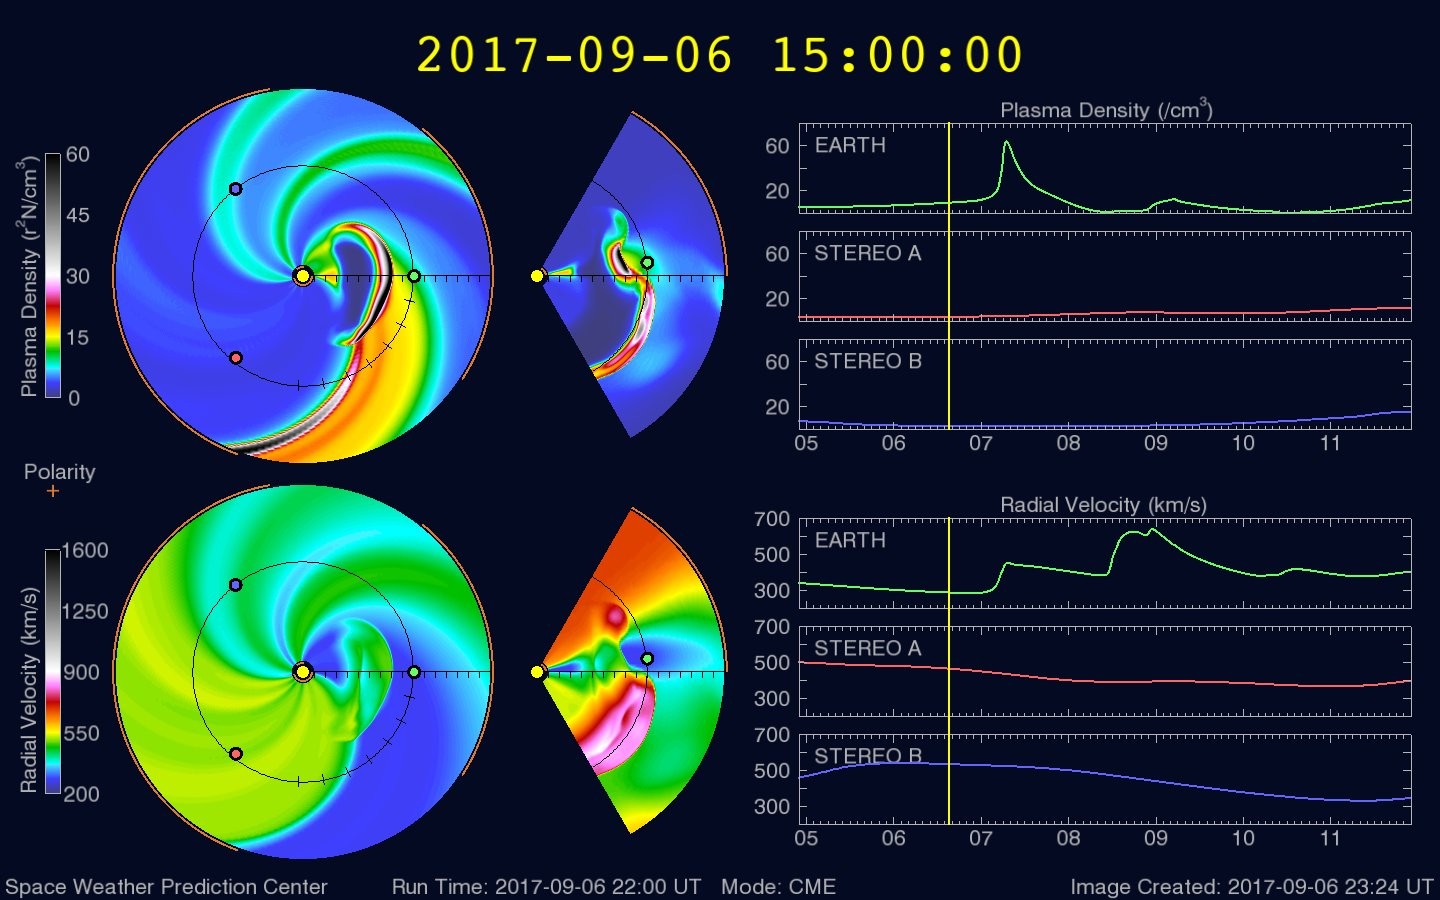
\includegraphics[width=\textwidth]{figures_of_others/images/enlil_com1_20170906T150000.jpg}
	\caption[\lofimage{figures_of_others/images/enlil_com1_20170906T150000.jpg}Credit: \href{http://dx.doi.org/10.7289/V5445JGH}{SWPC: WSA-Enlil Solar Wind Prediction. NOAA National Centers for Environmental Information}.]
	{Still frame of the WSA-Enlil model CME run for 6~September 2017. The top and bottom panels show the simulated values for the plasma density and the radial velocity respectively. The panels illustrate the inner heliosphere in the ecliptic plane, a slab of the polar plane, and the time evolution for the locations at Earth, STEREO~A and STEREO~B. The CME is shot into the ambient solar wind outflow produced by the open magnetic structure from the WSA interface. Credit: \href{http://dx.doi.org/10.7289/V5445JGH}{SWPC: WSA-Enlil Solar Wind Prediction. NOAA National Centers for Environmental Information}.}
	\label{fig:enlil_com1_20170906T150000}
\end{figure}
% https://www.ngdc.noaa.gov/enlil/

Precise solar wind predictions are very difficult to achieve, as it is already hard to trace solar wind measurements made at \SI{1}{\au} unambiguously back to its coronal source \citep{Cranmer2017}. Not only stream-stream interactions and internal solar wind processes, such as turbulence, complicate this, but interactions with CMEs as well.


\subsubsection*{CME forecast}
CMEs are already sighted raising from their source regions on the solar surface and some of their properties can be estimated from remote observations and modeled to Earth.
% CME forecast
Knowing the geometry of a CME, it is possible to infer its direction and speed from white-light images. Through kinematic forward-modeling techniques, that take advantage of the self-similar expansion observed in CMEs, it is possible to derive an estimated arrival time at Earth. As MCs are the drivers for most severe geomagnetic disturbances \citep{Bothmer1995,Cane2003}, it is also important to forecast their magnetic field strength and configuration.

% 3D models
An early 3D model for a general CME geometry is the ice-cream cone model, which assumes a simple bubble-like CME structure \citep{Fisher1984}. Though, building on the the white-light CME projection scheme study by \citet{Cremades2004}, \citet{Thernisien2006} created the more complex graduated cylindrical shell (GCS) model for flux rope-like CMEs. This model assumes an empirically derived electron distribution in order to create synthetic coronagraph images. The GCS model is successfully applied to images of CMEs with well-developed white-light structure \citep{Bosman2012} and is implemented as a part of current CME forecast procedures.

Early observations enable a heads-up time depending on the CME's propagation speed to Earth. This travel duration can be more than 4~days for slow events with average solar wind speeds, about 40~hours for fast events with speeds of \SI{1000}{\km\per\s}, and down to 20~hours and even below for the rare extreme cases, e.g., about 21~hours for the event on 23~July 2012 \citep{Russell2013,Temmer2015} and about 19~hours for the event observed by \citet{Carrington1859} on 1~September 1859.
% extreme events
Extreme CME velocities above \SI{2000}{\km\per\s} near the Sun are rare, nevertheless, in several cases speeds around \SI{3000}{\km\per\s} were measured. From the free energy available in active regions, \citet{Gopalswamy2005} concluded that CME speeds cannot be far greater than \SI{3000}{\km\per\s}. This would implicate that CMEs need at least half a day to travel from their source region on the Sun to reach Earth. \citet{Gopalswamy2010} even estimated a maximal limit of free energy active regions can store, which means that CMEs with \SI{4000}{\km\per\s} are not possible. Thus, the theoretical minimal heads-up time for CMEs is estimated to be half a day \citep{Gopalswamy2005}.

% CME kinematics
Calculating CME kinematics is a difficult task: Depending on whether CMEs are faster or slower than the surrounding solar wind, they decelerate/accelerate on their way through the heliosphere due to solar wind drag forces. Fast CMEs already decelerate substantially during their first few solar radii \citep{Sachdeva2017}. In case a CME interacts with a preceding CME, they both travel on with an intermediate speed \citep{Manoharan2004,Temmer2012}.
The average prediction errors of CME arrival times are still within a range of 14--20~hours and they also deteriorate with increasing solar activity \citep{Vrsnak2014}. The average difference between CME forecast times and arrival times was about 15~hours in 2017 -- for predictions submitted to the CME~Scoreboard\footnote{CCMC's CME~Scoreboard website: \urlfoot{https://kauai.ccmc.gsfc.nasa.gov/CMEscoreboard/}} which is developed by the Community Coordinated Modeling Center (CCMC).

% magnetic field forecast
Geomagnetic activity predictions benefit from an inferred magnetic field strength and direction along the line Earth passes through the CME \citep{Savani2017}.
Fast CMEs usually come with high magnetic field strengths as well, for example the CME observed by STEREO~A on 23~July 2012 had a shock speed of about \SI{2000}{\km\per\s} at \SI{1}{\au} and its magnetic field magnitude reached values of up to \SI{100}{\nT} \citep{Russell2013}.

% magnetic substructures
It is clear that geomagnetic storms can directly be attributed to the substructures of CMEs. The shock causes a sudden commencement, though the interior structures create geomagnetic storms if carrying a significant southward magnetic field. \citet{Tsurutani1988} showed that the compressed solar wind field in the sheath region behind the shock and the magnetic flux rope field are of equal importance for the generation of geomagnetic storms. Thus, the magnetic field vectors in the flux rope as well as in the sheath need to be forecasted.
% flux rope and sheath prediction
There are effective efforts to predict the direction and strength of the magnetic field from the remotely determined geometry and orientation of the flux rope \citep{Savani2015}. However, geomagnetic activity caused by MCs is easier to model than that caused by the compressed magnetic field in CME sheath regions or post-shock streams \citep{Huttunen2004}. One important reason is that the solar wind's $B_\text{z}$ component is quite random -- it has a much lower autocorrelation time than the $B_\text{x}$ and $B_\text{y}$ components, which makes $B_\text{z}$ also more difficult to forecast using prior values \citep{Elliott2013}. In fact, a remote prediction of the IMF direction in compression regions is not yet implemented into current forecasts. This is one reason why the intensity and duration of geomagnetic storms still cannot be predicted reliably from remote solar observations only.

% CME forecast methods and models
There exist multiple methods to forecast the CME arrival parameters at Earth, see the CCMC's CME~Scoreboard. However, methods that routinely forecast CMEs do not include internal magnetic structures and shocks \citep{Savani2015}. One prominent method is the implementation of a plasma cloud into the WSA-Enlil solar wind model, where the size and direction of the cloud is derived from remote solar images \citep{Zheng2013} -- this is done in the WSA-Enlil CME run displayed in \autoref{fig:enlil_com1_20170906T150000}.

A recently proposed method includes the prediction of the magnetic flux rope configuration inside a CME \citep{Savani2015}. It applies the adjusted BSS-scheme to obtain the initial magnetic configuration of the flux rope at the Sun. The direction and orientation of the CME is then modeled with the GCS-model. A simple model of a constant-alpha force-free flux rope \citep{Burlaga1988} is finally fit into a determined MC volume of influence. This procedure allows the construction of a magnetic field time series predicted for hitting Earth.


